\documentclass[oneside, 12pt]{book}
\usepackage{icdthesisUTF}
\usepackage{tabularx}
\usepackage[table]{xcolor} 
\usepackage{epsfig}
\usepackage{biblatex}
\usepackage{tikz}
\usepackage{tikz-uml}
\usepackage{sidecap}
\usepackage{wrapfig}
\usepackage{titlesec}
\usepackage{caption}
\usepackage{subcaption}
\usepackage{float}
\usepackage{amsmath}
\usepackage{listings}
\usepackage{longtable}

\usetikzlibrary{shapes.geometric, shapes.symbols, shapes.arrows, arrows.meta}

\renewcommand{\thesistitle}{Εξαγωγή δεδομένων τουριστικού ενδιαφέροντος από δημόσια APIs (Tourist-relevant data extraction from public APIs)}
\renewcommand{\thesisauthor}{Κωνσταντίνου Μαντζαβέλα (4056)}
\renewcommand{\thesisauthorabbrv}{Κ. Μαντζαβέλας}
\renewcommand{\thesisauthorinitials}{ΚΜ}
\renewcommand{\thesissupervisor}{Δρ. Νικόλαος Πεταλίδης}
\renewcommand{\thesismonth}{Μάιος}
\renewcommand{\thesisyear}{2020}
\tikzstyle{startstop} = [rectangle, rounded corners, minimum width=3cm, minimum height=1cm,text centered, draw=black, fill=blue!25, text width=6cm]

% Η βιβλιογραφία
\addbibresource{myThesis.bib}

\begin{document}
% Υποχρεωτικά τα παρακάτω:
\Titlepage
\Declarationpage
\begin{Abstract}
Στόχος αυτής της πτυχιακής εργασίας ήταν η εξαγωγή κάποιων πληροφοριών από δημόσια APIs, οι οποίες θα ήταν ιδιαίτερα χρήσιμες για έναν τουρίστα. 

Πιο συγκεκριμένα, αναπτύχθηκε ένας web server και μία εφαρμογή για κινητά Android η οποία μπορεί να χρησιμοποιηθεί από έναν τουρίστα στα ταξίδια του. Η εφαρμογή χρησιμοποιώντας τις πληροφορίες που εξήγαγε από κάποια δημόσια APIs έκανε διάφορες προτάσεις στον χρήστη για τις τοποθεσίες που θα μπορούσε να επισκεφθεί βάσει των ενδιαφερόντων του.

Παραδείγματος χάρη, η εφαρμογή προτείνει σε έναν χρήστη τις δημοφιλέστερες τοποθεσίες μιας πόλης βάσει του πλήθους των φωτογραφιών που έχουν τραβηχτεί σε κάθε τοποθεσία. Επίσης, ο χρήστης έχει τη δυνατότητα να αναζητήσει τοποθεσίες βάσει κατηγοριών (όπως αξιοθέατα) ή βάσει της δημοτικότητας των τοποθεσιών ανά εποχή του χρόνου.

Στην πτυχιακή εργασία αναλύονται οι λειτουργίες της εφαρμογής οι οποίες αναπτύχθηκαν καθώς και η ευέλικτη μεθοδολογία με την οποία οργανώθηκε και υλοποιήθηκε το project. Τέλος, αναφέρονται φυσικά και τα APIs τα οποία χρησιμοποιήθηκαν για την εξαγωγή πληροφοριών καθώς και τα συστήματα που βοήθησαν στην απρόσκοπτη ανάπτυξη του project (όπως το Jenkins για CI/CD).
\end{Abstract}
\tableofcontents

%Μόνο εφόσον θέλετε χωριστό πίνακα για εικόνες και πίνακες
\listoftables
\listoffigures

%Προαιρετικά
\begin{Acknowledgement}
Θα ήθελα να εκφράσω την βαθιά και ειλικρινή μου ευγνωμοσύνη για τον επιβλέποντα της πτυχιακής εργασίας, Δρ Νικόλαο Πεταλίδη, Καθηγητή, Επιστημονικό Συνεργάτη που μου έδωσε την ευκαιρία να εργαστώ σε ένα τόσο ενδιαφέρον θέμα όπου απέκτησα τριβή για πρώτη φορά με την επιστημονική κοινότητα και ήρθα σε επαφή  με τεχνολογίες και πρακτικές που χρησιμοποιούνται ευρέως στα επαγγελματικά περιβάλλοντα. Επίσης, θα ήθελα να τον ευχαριστήσω για την στήριξη και τη βοήθεια που μου παρείχε καθ' όλη τη διάρκεια ανάπτυξης της παρούσας πτυχιακής εργασίας. Η στήριξη του δεν ήταν μόνο στην παρούσα πτυχιακή εργασία, αλλά και κατά τη διάρκεια των σπουδών στα μαθήματα του στα οποία μας στήριζε, μας ενέπνευσε, μας συμβούλευε και μας καθοδηγούσε για θέματα ακαδημαϊκά αλλά και προγραμματιστικά. Ουσιαστικά μας προετοίμασε μέσω των μαθημάτων του για τα πρώτα επαγγελματικά βήματα που θα κάνουμε μετά από τις σπουδές μας. Για όλους αυτούς τους λόγους θα ήθελα να εκφράσω την ευγνωμοσύνη μου και τον θαυμασμό μου.

Τέλος, θα ήθελα να ευχαριστήσω την οικογένεια μου που με στήριξε σε όλα τα στάδια της ζωής μου και έκανε θυσίες ώστε να μπορέσω να σπουδάσω και να κάνω τα πρώτα μου επαγγελματικά βήματα. Επίσης, δεν μπορώ να παραλείψω από τις ευχαριστίες τους κοντινούς μου ανθρώπους και φίλους οι οποίοι με τη σειρά τους με στήριζαν και με ωθούσαν να προοδεύω κατά την διάρκεια των σπουδών μου αλλά και μετέπειτα.
\end{Acknowledgement}

%Προαιρετικά
\begin{Definitions}
Ορισμοί εννοιών που μπορεί να είναι χρήσιμοι. Για παράδειγμα:

\begin{description}
\item [Web Service] Λογισμικό που επιτρέπει την επικοινωνία δύο συστημάτων μέσω του Παγκόσμιου Ιστού.
\end{description}

\begin{description}
\item [XML] Γλώσσα σήμανσης που περιέχει ένα σύνολο κανόνων για την ηλεκτρονική κωδικοποίηση κειμένων
\end{description}

\begin{description}
\item [User Story] Η απλή περιγραφή μιας λειτουργίας ενός λογισμικού
\end{description}

\begin{description}
\item [Product Backlog] Μία ανάλυση των εργασιών που πρέπει να γίνουν σε μία ομάδα που εφαρμόζει Scrum.
\end{description}

\begin{description}
\item [Push Notification] Τα μηνύματα που γίνονται ``push'' από έναν server ή εφαρμογή σε μία διεπαφή χρήστη.
\end{description}

\begin{description}
\item [Framework] Λογισμικό που παρέχει μία γενικευμένη λειτουργικότητα που επεκτείνεται από κώδικα που γράφεται χρησιμοποιώντας αυτό.
\end{description}

\begin{description}
\item [Endpoint] Μία διεπαφή που παρέχεται από ένα μέσο επικοινωνίας ή μία υπηρεσία.
\end{description}

\end{Definitions}

%Από εδώ αρχίζει το κείμενό σας
\chapter{Εισαγωγή}
\section{Εφαρμογές τουριστικού περιεχομένου}
Η εξέλιξη των έξυπνων κινητών τηλεφώνων (smartphones) και η συνεχής ανάπτυξη εφαρμογών για αυτά, 
μεταξύ άλλων έχει διευκολύνει αρκετά τους τουρίστες στην οργάνωση των ταξιδιών τους.
Επίσης, η ευκολία εύρεσης αυτών των πληροφοριών οπουδήποτε και οποιαδήποτε στιγμή έχει συμβάλλει στην ανέλιξη χρήσης τέτοιων τουριστικών εφαρμογών σε κινητές συσκευές.
Άλλωστε, δεν είναι τυχαίο πως περίπου το 50 τοις εκατό των εφαρμογών τουριστικού περιεχομένου έχουν σχεδιαστεί για κινητές συσκευές.
Έχει συμβάλλει σημαντικά στην διευκόλυνση οργάνωσης ενός ταξιδιού. 
Πλέον, ο ταξιδιώτης έχει στη διάθεσή του ένα μεγάλο αριθμό εφαρμογών στο αποθετήριο της κινητής συσκευής του, 
με τις οποίες μπορεί να βρει πληροφορίες και να οργανώσει το ταξίδι και τις δραστηριότητες που τον ενδιαφέρουν.

\section{Κατηγορίες τουριστικών εφαρμογών}
Υπάρχουν τέσσερις (4) βασικές κατηγορίες στις οποίες κατατάσσονται οι mobile τουριστικές εφαρμογές. 
Αυτές είναι οι :
\begin{itemize}
    \item Online Booking
    \item Information Resource
    \item Location-Based Υπηρεσίες
    \item Trip Journal
\end{itemize}
Στην κατηγορία ``Location-Based Υπηρεσιών'' ανήκουν οι εφαρμογές 
που προσφέρουν στον χρήστη πληροφορίες βάσει της τρέχουσας τοποθεσίας 
του (πχ πλοήγηση, πληροφορίες για κοντινά νοσοκομεία).
\cite{smirnov2014mobile}
Η εφαρμογή της παρούσας πτυχιακής εργασίας ανήκει στην κατηγορία 
``Location-Based Υπηρεσιών'' καθώς προτείνει στον χρήστη διάφορα 
αξιοθέατα βάσει της τοποθεσίας του.

\section{Διαδεδομένες εφαρμογές τουριστικού περιεχομένου}
Παρομοίως με την εφαρμογή που αναπτύχθηκε για τις ανάγκες της παρούσας πτυχιακής, 
κυκλοφορούν αρκετές εμπορικές εφαρμογές τουριστικού περιεχομένου.
Οι πιο διαδεδομένες εφαρμογές που ανήκουν σε μία ή περισσότερες από τις κατηγορίες που αναφέρθηκαν παραπάνω είναι οι~\cite{Oprahmag_TravelApps}:

\begin{longtable}{|p{.2\textwidth}|p{.2\textwidth}|p{.5\textwidth}|}
\hline
Εφαρμογή & Πλατφόρμες & Σύντομη Περιγραφή\\
\hline
Hopper & Android \& iOS & Το Hopper συγκεντρώνει κάθε μέρα 
δισεκατομμύρια τιμές αεροπορικών εισιτηρίων και δωματίων ξενοδοχείων. 
Επίσης βάσει του ιστορικού του, προτείνει αν πρέπει ο χρήστης να 
προβεί άμεσα στην κράτηση ή να περιμένει να πέσει η τιμή. \\
\hline
Google Trips & Android \& iOS & Το Google Trips δημιουργεί το 
πρόγραμμα για το ταξίδι (ώρες πτήσης), καθώς και παρέχει διάφορες 
πληροφορίες όπως την ισοτιμία συναλλάγματος, τηλέφωνα έκτακτης ανάγκης 
(νοσοκομεία, αστυνομία) καθώς και μέρη που υπάρχει πρόσβαση σε Wi-Fi.\\
\hline
Airbnb & Android \& iOS & Το Airbnb παρέχει υπηρεσίες ενοικίασης 
καταλυμμάτων βάσει διαφόρων φίλτρων. Ο χρήστης επιλέγει ενοικιαζόμενα βάσει το είδος του καταλύματος (δωμάτιο, διαμέρισμα) καθώς και βάσει προσωπικών προτιμήσεων (πισίνα, πλυντήριο, φιλικό προς κατοικίδια).\\ 
\hline
Hipmunk & Android \& iOS & Το Hipmunk προτείνει ταξίδια βάσει
κατηγοριών όπως ``ρομαντικά'', ``νυχτερινή ζωή'', ``απίστευτα νησιά'' κλπ.\\
\hline
Rome2rio & Android \& iOS & Ο χρήστης επιλέγει μία διεύθυνση, ένα 
αξιοθέατο ή μία πόλη και το Rome2rio προτείνει στο χρήστη καταλύματα 
και δραστηριότητες.\\
\hline
TripAdvisor & Android \& iOS & Στο TripAdvisor υπάρχουν εκατοντάδες 
εκατομμύρια κριτικές από εστιατόρια, ξενοδοχεία ή ακόμα και μουσεία.\\
\hline
\caption{Διαδεδομένες εφαρμογές τουριστικού περιεχομένου}
\label{table:famous_tourist_relevant_apps}
\end{longtable}


\chapter{Ανοιχτά Δεδομένα}
\section{Εισαγωγή}
Ως ανοιχτά, ορίζονται τα δεδομένα που μπορούν ελεύθερα να 
χρησιμοποιηθούν, να επαναχρησιμοποιηθούν και να αναδιανεμηθούν από 
οποιονδήποτε – υπό τον όρο να γίνεται αναφορά στους δημιουργούς και να διατίθενται, με τη σειρά τους, υπό τους ίδιους όρους.

Τα σημαντικότερα στοιχεία των ανοιχτών δεδομένων είναι τα εξής~\cite{OpenData_definition}:
\begin{itemize}
    \item \textbf{Διαθεσιμότητα και Προσβασιμότητα}: Τα δεδομένα 
    πρέπει να είναι διαθέσιμα αυτούσια, να έχουν ένα λογικό κόστος 
    αναπαραγωγής, και κατά προτίμηση να είναι διαθέσιμα για λήψη από 
    το Διαδίκτυο. Επίσης, πρέπει να είναι διαθέσιμα σε κάποια πρακτική 
    και παραμετροποιήσιμη μορφή.
    \item \textbf{Επαναχρησιμοποίηση και Αναδιανομή}: Τα δεδομένα 
    θα πρέπει να είναι διαθέσιμα υπό όρους που επιτρέπουν την 
    επαναχρησιμοποίηση και την αναδιανομή τους, συμπεριλαμβανομένης 
    και της ανάμειξης με άλλα σύνολα δεδομένων.
    \item \textbf{Καθολική Συμμετοχή}: Καθένας πρέπει να μπορεί 
    να χρησιμοποιήσει, να επαναχρησιμοποιήσει και να αναδιανείμει τα
    δεδομένα. Δεν πρέπει αυτά να υπόκεινται σε διακρίσεις με βάση τον 
    τομέα δραστηριότητας ή τα πρόσωπα και τις ομάδες. Για παράδειγμα, 
    περιορισμοί για «μη-εμπορική χρήση» ή περιορισμοί για χρήση μόνο 
    για συγκεκριμένους σκοπούς (π.χ. μόνο στην εκπαίδευση) δεν είναι 
    επιτρεπτοί.
\end{itemize}


\section{Παράδειγμα χρήσης Ανοιχτών Δεδομένων}
Παρακάτω παρατίθεται ένα παράδειγμα για να αναδειχθεί η
χρησιμότητα των Ανοιχτών Δεδομένων.
Ας πάρουμε το παράδειγμα ενός κρατικού προϋπολογισμού, ο οποίος 
αποτελείται από εκατοντάδες διαφορετικούς πίνακες, όλοι τους με μία 
μικρή διαφοροποίηση στη διάταξη.
Για να γίνει μία ανάλυση των κονδυλίων σε διαφορετικές κατηγορίες από 
αυτές που επέλεξε ο εκδότης, οι πολίτες θα έπρεπε να μεταφέρουν 
χειροκίνητα όλα αυτά τα δεδομένα σε ένα νέο έγγραφο. Για έναν κρατικό 
προϋπολογισμό, αυτό θα μπορούσε να είναι αρκετά χρονοβόρο και να διαρκέσει πολλές εβδομάδες.
Ακόμη και όταν ολοκληρωθεί η διαδικασία της μεταφοράς αυτών των 
δεδομένων, οι πολίτες μπορεί να ανακάλυπταν ότι τα δεδομένα 
προστατεύονται από πνευματικά δικαιώματα όπου απαγορεύεται η ευρεία 
χρήση αυτών των δεδομένων.

Αυτό το πρόβλημα καλούνται να λύσουν τα ανοιχτά δεδομένα.
Μία ανάλυση προϋπολογισμού ενός κράτους, θα επέτρεπε στους πολίτες να 
χρησιμοποιήσουν αυτά τα δεδομένα με οποιοδήποτε τρόπο επιθυμούν.
Οι προγραμματιστές θα μπορούσαν να χρησιμοποιήσουν αυτά τα δεδομένα 
ώστε να παρέχουν στους πολίτες εφαρμογές που θα τους ήταν περισσότερο 
χρήσιμες, αξιοποιώντας αυτά τα δεδομένα.
Τέλος, οι δυνατότητες της χρήσης αυτών των δεδομένων περιορίζονται 
μόνο από την φαντασία της κοινότητας που θα τα χρησιμοποιήσει~\cite{davies2012might}.

\section{Χρήση των Ανοιχτών Δεδομένων στο TripAssistant}
Στην εφαρμογή TripAssistant χρησιμοποιήθηκαν ανοιχτά δεδομένα για τις 
φωτογραφίες που φορτώθηκαν από το API του Flickr. Οι φωτογραφίες 
αυτές χρησιμοποιήθηκαν στην εφαρμογή για την εξαγωγή διαφόρων 
στατιστικών που ήταν χρήσιμα για τους χρήστες. Επίσης οι 
φωτογραφίες αυτές προβλήθηκαν σε κάποια σημεία της εφαρμογής.
\newpage
Επειδή οι φωτογραφίες που φορτώθηκαν από το API του Flickr 
ανεβαίνουν όλες από χρήστες, ενδέχεται να υπόκεινται σε 
πνευματικά δικαιώματα. Η εφαρμογή Trip Assistant, φόρτωσε μέσω του 
API μόνο φωτογραφίες οι οποίες υπόκεινται στο Attri\-bution License, 
δηλαδή είναι ανοιχτές προς αντιγραφή, διανομή, προβολή. Οι φωτογραφίες αυτές καθώς και οι άδειες διάθεσής τους περιγράφονται 
στην ιστοσελίδα~\url{https://www.flickr.com/creativecommons}.

\chapter{Εισαγωγή στα REST APIs}
\section{Ορισμός του API}
Ένα μέρος της συγκεκριμένης πτυχιακής εργασίας είναι η άντληση δεδομένων από δημόσια APIs.
Οπότε χρειάζεται να γίνει μία αναφορά στον ορισμό του API.
Αρχικά, ένα API είναι ένα σύνολο από μεθόδους που ορίζουν την επικοινωνία μεταξύ συστημάτων. Τα APIs διατίθενται σε προγραμματιστές ώστε να τους διευκολύνουν στην ανάπτυξη προγραμμάτων διαφόρων σκοπών.
Τέτοια APIs μπορεί να αφορούν κάποιο λειτουργικό σύστημα, σύστημα βάσεων δεδομένων, υλικό (hardware) υπολογιστών αλλά και κάποιο διαδικτυακό σύστημα.

Κάποια παραδείγματα APIs που χρησιμοποιούνται ευρέως είναι το Windows API και το POSIX.
Συνήθως μαζί με το API διατίθεται ένα εγχειρίδιο που περιγράφει τα use cases του API αλλά και οδηγίες για την υλοποίησή του.

\section{Ορισμός των REST APIs}
Το Representational State Transfer (REST) είναι μία αρχή στην αρχιτεκτονική λογισμικού που καθορίζει ένα σύνολο από περιορισμούς που χρησιμοποιούνται κατά την ανάπτυξη Web Services. Τα REST Web Services είναι ένα υποσύνολο του Παγκόσμιου Ιστού (WWW) και είναι βασισμένα στο πρωτόκολλο HTTP.  

Τα βασικά χαρακτηριστικά των REST APIs είναι τα εξής~\cite{fielding_rest}:
\begin{itemize}
    \item χρήση της \textbf{αρχιτεκτονικής Client-Server}:
    Η βασική ιδέα πίσω από την αρχιτεκτονική Client-Server είναι ο 
    διαχωρισμός του προγράμματος σε επιμέρους ξεχωριστά τμήματα.
    Διαχωρίζοντας το τμήμα της διεπαφή χρήστη από το τμήμα της 
    αποθήκευσης των δεδομένων επιτυγχάνεται η φορητότητα του 
    προγράμματος και η επεκτασιμότητα.
    \item \textbf{Stateless}: η επικοινωνία μεταξύ client και server 
    πρέπει να είναι stateless, δηλαδή να μην κρατηθεί καμία πληροφορία 
    για την κατάσταση του client. Κάθε request από τον client στον 
    server πρέπει να περιέχει όλες τις απαραίτητες πληροφορίες ώστε ο 
    server να κατανοήσει το request.
    \item \textbf{Cache}: Χρησιμοποιώντας cache στον client 
    βελτιώνεται η απόδοση του δικτύου. Τα δεδομένα που επιστρέφει ο 
    server σε μία απάντηση (response) πρέπει να χαρακτηρίζονται από 
    τον client σαν cacheable ή non-cacheable. Εάν μία απάντηση είναι 
    cacheable, τότε ο client μπορεί να επαναχρησιμοποιήσει αυτά τα 
    δεδομένα αργότερα. Με αυτό τον τρόπο, μειώνεται ο φόρτος του 
    δικτύου μαζί με τις αλληλεπιδράσεις μεταξύ client-server, όπως 
    επίσης βελτιώνεται η εμπειρία χρήστη.
    \item \textbf{Ενιαία Διεπαφή (Uniform Interface)}: Το κύριο 
    χαρακτηριστικό που ξεχωρίζει την αρχιτεκτονική REST από τις 
    υπόλοιπες, είναι η έμφαση που δίνεται στην χρήση μιας ενιαίας 
    διεπαφής μεταξύ των τμημάτων του λογισμικού. Εφαρμόζοντας αυτή την 
    αρχή, η αρχιτεκτονική ενός συστήματος απλουστεύεται σημαντικά. 
    Επίσης, οι εκάστοτε υλοποιήσεις διαχωρίζονται από τις υπηρεσίες που 
    προσφέρουν. Η διεπαφή REST έχει σχεδιαστεί να είναι αποδοτική στη 
    μεταφορά μεγάλων όγκων δεδομένων, κάτι που την καθιστά βέλτιστη 
    λύση για την περίπτωση του Web.
    \item \textbf{Στρωματοποιημένο Σύστημα (Layered System)}:
    Σε αυτή την αρχιτεκτονική, το κάθε στρώμα αποτελείται από τμήματα 
    (components) που δεν μπορούν να ``δουν'' πέρα από το στρώμα με το 
    οποίο αλληλεπιδρούν άμεσα. Περιορίζοντας την γνώση του συστήματος 
    σε ένα στρώμα, μπαίνει ένα όριο στην συνολική πολυπλοκότητα του 
    συστήματος.
\end{itemize}


\section{Τα δημόσια API}
Τα δημόσια APIs (public APIs ή open APIs) είναι οι διεπαφές 
προγραμματισμού εφαρμογών (APIs) που διατίθενται δωρεάν προς χρήση σε 
προγραμματιστές.
Τέτοια APIs παρέχουν στους προγραμματιστές που τα χρησιμοποιούν 
πρόσβαση σε κάποια ιδιωτική εφαρμογή ή κάποιο web service.
Τα APIs τα οποία διανέμουν web services υλοποιούνται στη μεγάλη τους 
πλειοψηφία σε SOAP ή REST. Η παρούσα πτυχιακή χρησιμοποιεί διάφορα 
REST public APIs.

Οι κύριες διαφορές των SOAP με τα REST web services είναι ότι τα SOAP 
παρόλο που είναι μια ευρέως διαδεδομένη και παλιά τεχνολογία,  έχουν 
μεγαλύτερο φορτίο δεδομένων σε σχέση με το REST. Επίσης τα SOAP 
services επιστρέφουν αυστηρώς XML δεδομένα σε αντίθεση με τα REST που 
είναι πιο ευέλικτα ως προς τον τύπο των δεδομένων που θα επιστρέψουν. 
Επιπρόσθετα τα SOAP web services χρησιμοποιούν παραπάνω bandwidth 
καθώς μία απάντηση σε SOAP μπορεί να χρειαστεί μέχρι και 10 φορές 
περισσότερα byte συγκριτικά με το REST. Τέλος το SOAP είναι το 
πρότυπο που επικρατεί για τα web services οπότε και έχει καλύτερη 
υποστήριξη από άλλα πρότυπα (WSDL, WS)~\cite{wagh2012comparative}

\section{Πλεονεκτήματα των δημοσίων APIs}
Το σημαντικότερο πλεονέκτημα των δημοσίων APIs είναι ότι διατίθενται 
δωρεάν χωρίς κάποιον περιορισμό στην χρήση τους. Μπορεί δηλαδή μία 
εταιρεία ή ένας προγραμματιστής να χρησιμοποιήσει ένα δημόσιο API στην 
εφαρμογή του και να ξεκινήσει την εμπορική διάθεση του λογισμικού του.
Παράλληλα ο εκδότης του δημοσίου API κρατά υπό την δικαιοδοσία του τον 
πηγαίο κώδικα του API ενώ παράλληλα ωφελείται από την αύξηση της 
βάσεως των χρηστών του.

Παρόλα αυτά τα δημόσια APIs πρέπει να αντιμετωπίζονται από τους εκδότες 
τους ως τελικό προϊόν καθώς μπορούν να επηρεάσουν τη φήμη του 
οργανισμού είτε θετικά είτε αρνητικά.
Ο οργανισμός που διαθέτει ένα δημόσιο API πρέπει να έχει διασφαλίσει 
ότι το API:
\begin{itemize} %check if i can use description for this
\item Δεν περιέχει bugs 
\item Δεν έχει κενά ασφαλείας
\item Δεν εκθέτει προσωπικά δεδομένα
\end{itemize}

\section{Μειονεκτήματα των δημοσίων APIs}
Το σημαντικότερο μειονέκτημα των δημοσίων API είναι το γεγονός πως ο 
οργανισμός που τα εκδίδει μπορεί ανά πάσα στιγμή να αλλάξει τους όρους 
χρήσης και να ορίσει κάποιο αντίτιμο για την χρήση του API. Σε αυτή 
την περίπτωση οι προγραμματιστές που το χρησιμοποιούν δεν έχουν άλλη 
επιλογή παρά να το αποδεχτούν.

\section{Τα REST APIs που χρησιμοποιήθηκαν}
Στην εφαρμογή TripAssistant χρησιμοποιήθηκαν κατά κύριο λόγο τρία 
δημόσια REST APIs.
Σε όλες τις παρακάτω περιπτώσεις χρησιμοποιήθηκε το JSON ως media type.

\subsection{Flickr API}
Το API του flickr χρησιμοποιήθηκε για τον σκοπό της συγκέντρωσης 
γεωαναγραφόμενων φωτογραφιών από μία συγκεκριμένη πόλη.
Συγκεντρώνονται όλες οι φωτογραφίες που έχουν ανέβει στο Flickr τα 
τελευταία 3 χρόνια και σώζονται σε μία βάση δεδομένων κρατώντας τις 
γεωγραφικές συντεταγμένες της φωτογραφίες, έναν σύνδεσμο της 
φωτογραφίας από το flickr μαζί με κάποιες ακόμα πληροφορίες.

Το κεντρικό URL που χρησιμοποιήθηκε για το 
API του flickr είναι το \textbf{https://api.flickr.com} 
Τα endpoints που χρησιμοποιήθηκαν είναι τα εξής:
\begin{itemize}
    \item \textbf{/services/rest?method=flickr.photos.search\&lat=40.23124\&lon=21.12342\\\&has\_geo=1\&min\_upload\_date=1449867647}
    
    \textbf{Μέθοδος}: GET
    
    Επιστρέφει μία λίστα από φωτογραφίες που πληρούν κάποια κριτήρια.
    Συγκεκριμένα τα κριτήρια που έχουν τεθεί στο παραπάνω παράδειγμα 
    είναι οι φωτογραφίες που έχουν γεωπληροφορίες, που βρίσκονται 
    κοντά στις ζητούμενες γεωγραφικές συντεταγμένες και η ημερομηνία 
    που μεταφορτώθηκαν είναι μεγαλύτερη της ζητούμενης (δίνεται epoch time φορμάτ).
    
    Documentation: \url{https://www.flickr.com/services/api/flickr.photos.search.html}
    \item \textbf{/services/rest?method=flickr.photos.getInfo\&photo\_id=12345\\\&secret=ab32cd1ef}
    
    \textbf{Μέθοδος}: GET
    
    Επιστρέφει περισσότερες πληροφορίες για την φωτογραφία με 
    το id που ζητήθηκε.
    
    Documentation: \url{https://www.flickr.com/services/api/flickr.photos.getInfo.html}
\end{itemize}

\subsection{Facebook Graph Places Search API}\label{sec:facebook_graph_places_api}
Το Places Search API του Facebook χρησιμοποιήθηκε για να διασταυρωθούν 
αλλά και να ενισχυθούν οι υπάρχουσες πληροφορίες τοποθεσιών.
Για ένα ζευγάρι γεωγραφικών συντεταγμένων, καλείται το API του 
Facebook ώστε να ενισχυθούν οι υπάρχουσες πληροφορίες για μία 
τοποθεσία όπως η περιγραφή, οι κατηγορίες της τοποθεσίας, η 
επισκεψιμότητα της τοποθεσίας (check-ins κατά το facebook), καθώς και το όνομα της ευρύτερης περιοχής. 
Το endpoint που χρησιμοποιήθηκε είναι το εξής:
\begin{itemize}
    \item \textbf{https://graph.facebook.com/v5.0/search?type=place\\\&center=40.6152792,22.9607157\&distance=50\\\&fields=id,name,about,description,checkins,location,category\_list\\\&access\_token=123456789012345|5426dc78123ed241460393f694448fba}
    
    \textbf{Μέθοδος}: GET
    
    Επιστρέφει μία λίστα από τις τοποθεσίες που είναι κοντά στα 50 
    μέτρα από το κέντρο των γεωγραφικών συντεταγμένων που δόθηκαν.
    Η λίστα περιέχει τοποθεσίες οι οποίες έχουν πληροφορίες όπως 
    όνομα, περιγραφή, αριθμός επισκέψεων (check-ins), τοποθεσία (Πόλη, 
    Χώρα, γεωγραφικές συντεταγμένες) και κατηγορίες.
    
    Documentation: \url{https://developers.facebook.com/docs/places/web/search/}
\end{itemize}
 
\subsection{DataMuse API}\label{sec:datamuse_api_call}
To API του DataMuse είναι μία μηχανή εύρεσης λέξεων. Παρέχοντας μία 
λέξη, επιστρέφει μία λίστα από λέξεις που νοηματικά βρίσκονται κοντά ή 
είναι ίδιες. Επίσης, μπορούν να καθοριστούν διάφορες παράμετροι όπως ο 
συλλαβισμός, ο ήχος και το λεξιλόγιο. 
Το endpoint που χρησιμοποιήθηκε είναι το εξής:
\begin{itemize}
    \item \textbf{https://api.datamuse.com/words?ml={word}} 
    
    \textbf{Μέθοδος}: GET
    
    Επιστρέφει μία λίστα από λέξεις με σημασία παρόμοια με την λέξη {word}
    
    Documentation: \url{https://www.datamuse.com/api/}
\end{itemize}

\chapter{Διαχείριση Έργου}
\section{Αρχική ερεύνα}
Για την καλύτερη οργάνωση και διαχείριση του συγκεκριμένου project χρησιμοποιήθηκαν κάποιες αρχές της ευέλικτης μεθοδολογίας Scrum.

Το ελάχιστο που χρειάζεται για να ξεκινήσει ένα Scrum project είναι να 
υπάρχει ένα όραμα και ένα Product Backlog.
Συγκεκριμένα το όραμα περιγράφει το λόγο που αναλήφθηκε το project και ποιο είναι το επιθυμητό αποτέλεσμα~\cite{schwaber2004agile}.

Στην αρχή ενός έργου, οι προγραμματιστές και οι πελάτες συζητάνε 
για το νέο σύστημα με σκοπό να καθορίσουν όλες τις βασικές και 
σημαντικές λειτουργίες. 
Ωστόσο, δεν χρειάζεται να καθοριστούν όλες οι λειτουργίες της 
εφαρμογής. Καθώς το έργο προχωράει, οι πελάτες συνεχίζουν να 
ανακαλύπτουν καινούργιες λειτουργίες.
Καθώς καθορίζεται μία λειτουργία, διασπάται σε ένα ή περισσότερα user stories τα οποία γράφονται το καθένα σε μία 
καρτέλα. Σε κάθε καρτέλα γράφεται μόνο το όνομα του story όπως για 
παράδειγμα ``Δημιουργία Χρήστη''. Δεν χρειάζονται λεπτομέρειες πάνω στην 
καρτέλα, παρά μόνο μια υπενθύμιση των λειτουργιών.

Έπειτα, οι προγραμματιστές κάνουν μία εκτίμηση των user stories. 
Ένας αριθμός ``points'' (πόντων) γράφεται πάνω σε κάθε καρτέλα story 
ο οποίος αναπαριστά το σχετικό κόστος του story. Μπορεί να μην 
είναι ακόμα γνωστό τι χρονική διάρκεια αναπαριστά κάθε story point, 
αλλά είναι γνωστό ότι ένα story με 8 points (πόντους) θα διαρκέσει 
2 φορές παραπάνω από ένα story με 4 points.
Όλα αυτά τα stories, στο τέλος τοποθετούνται στο backlog του project μαζί και με τα μελλοντικά stories~\cite[Chapter~3]{AgilePrinciplesC}.

\section{Καθορισμός Επαναλήψεων}
Αφού έχουν καθοριστεί οι βασικές λειτουργίες και τα stories, επόμενο βήμα είναι να καθοριστεί το μέγεθος των επαναλήψεων που θα ακολουθηθεί.
Συνήθως, αυτός ο αριθμός είναι 1 ή 2 εβδομάδες, όπου οι πελάτες και οι 
προγραμματιστές καθορίζουν τα stories που θα μπουν σε κάθε επανάληψη.
Σημαντικό είναι σε κάθε επανάληψη να μην επιλεχθούν παραπάνω stories 
από όσα είναι δυνατόν να έρθουν σε πέρας, σύμφωνα με το velocity της 
ομάδας.
Επίσης οι πελάτες δεν έχουν τη δυνατότητα να αλλάξουν τα stories μιας 
επανάληψης αφού έχει ήδη ξεκινήσει.
Είναι ελεύθεροι να αλλάξουν ή αναδιατάξουν οποιοδήποτε άλλο story μέσα 
στο project, εκτός από αυτά που έχουν ξεκινήσει να δουλεύουν ήδη οι 
προγραμματιστές.
Επιπλέον, η επανάληψη τελειώνει στην προκαθορισμένη ημερομηνία, ακόμη 
και αν δεν έχουν ολοκληρωθεί όλα τα stories.
Στο τέλος της επανάληψης, επανακαθορίζεται το velocity της ομάδας 
αθροίζοντας τα story points που ολοκληρώθηκαν. Για παράδειγμα, εαν 
αυτός ο αριθμός είναι 31 τότε το velocity της ομάδας είναι 31 και στην 
επόμενη επανάληψη θα πρέπει να προστεθούν stories με 31 story points 
στο σύνολο.
\cite[Chapter~3]{AgilePrinciplesC}
\section{Τα stories της εφαρμογής}
Όπως περιγράφηκε προηγουμένως, κατά το ξεκίνημα του project 
καθορίστηκαν οι βασικές λειτουργίες της εφαρμογής οι οποίες 
αντιστοιχήθηκαν σε ένα ή περισσότερα stories η καθεμιά.
Τα stories που υπήρχαν στο backlog είναι τα παρακάτω.

User Stories:\vspace{0.5cm}

\begin{tikzpicture}[node distance=7cm]
\node (story1) [startstop] {\textbf{User Story 1} - Σαν χρήστης θέλω να δω τις 10 δημοφιλέστερες τοποθεσίες τριγύρω μου};
\node (story2) [startstop, right of=story1] {\textbf{User Story 2} - Σαν χρήστης θέλω να δημιουργήσω έναν λογαριασμό χρήστη και να συνδεθώ με αυτόν };
\end{tikzpicture}\vspace{0.5cm}

\begin{tikzpicture}[node distance=7cm]
\node (story3) [startstop] {\textbf{User Story 3} - Σαν χρήστης θέλω προτάσεις από τοποθεσίες σε μία ακτίνα τριγύρω μου, βάσει κατηγορίας};
\node (story4) [startstop, right of=story3] {\textbf{User Story 4} - Σαν χρήστης θέλω να προσθέσω τοποθεσίες σε ένα ταξίδι και να το προγραμματίσω για το μέλλον};
\end{tikzpicture}\vspace{0.5cm}

\begin{tikzpicture}[node distance=7cm]
\node (story3) [startstop] {\textbf{User Story 5} - Σαν χρήστης θέλω να γράφω αξιολόγηση για μία τοποθεσία που επισκέφθηκα αλλά και να διαβάζω τις αξιολογήσεις των υπόλοιπων χρηστών};
\node (story4) [startstop, right of=story3] {\textbf{User Story 6} - Σαν χρήστης θέλω να έχω τη δυνατότητα να συνομιλήσω μέσω chat με άλλους χρήστες στην ίδια πόλη που βρίσκομαι ώστε να μου προτείνουν μέρη να επισκεφθώ};
\end{tikzpicture}\vspace{0.5cm}

\begin{tikzpicture}[node distance=7cm]
\node (story3) [startstop] {\textbf{User Story 7} - Σαν χρήστης θέλω να μου προτείνει η εφαρμογή την βέλτιστη διαδρομή να ακολουθήσω από μία λίστα επιλεγμένων τοποθεσιών};
\node (story4) [startstop, right of=story3] {\textbf{User Story 8} - Σαν χρήστης θέλω να δω τις δημοφιλείς τοποθεσίες για την τρέχουσα εποχή του χρόνου κοντά μου};
\end{tikzpicture}\vspace{0.5cm}

\begin{tikzpicture}[node distance=7cm]
\node (story3) [startstop] {\textbf{User Story 9} - Σαν χρήστης θέλω να λάβω ειδοποίηση (push notification) στο κινητό μου για να μου υπενθυμίσει ένα ταξίδι που πλησιάζει};
\end{tikzpicture}\vspace{0.5cm}

Αξίζει να σημειωθεί πως από τα παραπάνω stories δεν υλοποιήθηκαν όλα, 
ωστόσο σε επόμενο κεφάλαιο θα αναλυθούν τα user stories και οι 
λειτουργίες που υλοποιήθηκαν.
Επιπλέον, τα περισσότερα από αυτά είχαν καθοριστεί στην αρχή του 
project όπου και τοποθετήθηκαν στο backlog.
Στη συνέχεια, όταν καταγραφόταν ένα καινούργιο user story που αφορούσε την υλοποίηση μίας νέας λειτουργίας, τότε προστίθετο στο backlog με τη σειρά του.
\section{Releases}
Στον μέχρι τώρα κύκλο ζωής του project, κυκλοφόρησαν 6 releases.
Όλα τα releases φιλοξενήθηκαν στο αποθετήριο της εφαρμογής που φιλοξενείται στον ιστότοπο του Github στον σύνδεσμο \url{https://github.com/kostasmantz/trip-assistant/releases}. 
Ο πηγαίος κώδικας της εφαρμογής διατίθεται υπό την άδεια ανοιχτού λογισμικού Apache License 2.0 .
Τα releases και οι λειτουργίες που περιλαμβάνουν περιγράφονται παρακάτω.

{\large \color{blue}{TripAssistant 0.1.0}}
\begin{enumerate}
    \item Εξαγωγή των 10 δημοφιλέστερων τοποθεσιών μιας πόλης, απ'το σύνολο των φωτογραφιών που έχουν ανέβει εκεί.
    \item Υλοποίηση ενός web service που παρέχει τις 10 δημοφιλέστερες τοποθεσίες μιας πόλης, βάσει των γεωγραφικών συντεταγμένων του χρήστη.
\end{enumerate}

{\large \color{blue}{TripAssistant 0.2.0}}
\begin{enumerate}
    \item Εγγραφή και σύνδεση των χρηστών στην εφαρμογή.
    \item Εύρεση προτάσεων από τοποθεσίες κοντά στον χρήστη βάσει κατηγορίας τοποθεσίας.
    \item Χρήση του προσθέτου Jacoco για την παραγωγή αναφορών Unit και Integration tests.
\end{enumerate}

{\large \color{blue}{TripAssistant 0.3.0}}
\begin{enumerate}
    \item Δημιουργία και προγραμματισμός ενός ταξιδιού για το μέλλον.
    Τοποθέτηση τοποθεσιών στο μελλοντικό ταξίδι.
\end{enumerate}

{\large \color{blue}{TripAssistant 0.4.0}}
\begin{enumerate}
    \item Υλοποίηση ειδοποιήσεων push (push notifications) για προγραμματισμένα ταξίδια που πλησιάζουν.
    \item Διόρθωση διαφόρων bugs.
    \item Μικρές βελτιώσεις στην σχεδίαση.
\end{enumerate}

{\large \color{blue}{TripAssistant 0.5.0}}
\begin{enumerate}
    \item Εξαγωγή και πρόταση δημοφιλών τοποθεσιών για την τρέχουσα εποχή του χρόνου.
    \item Διόρθωση διαφόρων bugs.
    \item Βελτιώσεις στον κώδικα.
\end{enumerate}

{\large \color{blue}{TripAssistant 0.6.0}}
\begin{enumerate}
    \item Χρήση της αναβαθμισμένης έκδοσης του Facebook API για αναζήτηση τοποθεσιών.
    \item Ενημέρωση του README αρχείου του project.
    \item Χρήση του SonarQube με σκοπό την ανάλυση του πηγαίου κώδικα.
    \item Διόρθωση bugs.
\end{enumerate}

Η λογική της δημιουργίας των παραπάνω εκδόσεων ακολουθεί την 
στρατηγική του Semantic Versioning. Επιλέχθηκε η συγκεκριμένη 
στρατηγική μεταξύ άλλων, καθώς είναι αρκετά ξεκάθαρη και απλή η 
εφαρμογή της.
Το Semantic Versioning, χρησιμοποιεί μία ακολουθία από τρία ψηφία Major.Minor.Patch (Μείζων.Ελάσσον.Μπάλωμα).
Σε αυτή τη στρατηγική ισχύουν οι εξής απλοί κανόνες~\cite{preston2013semantic}.
\begin{enumerate}
    \item Η Major έκδοση, αυξάνεται όταν γίνονται ασύμβατες αλλαγές στο API. 
    \item Η Minor έκδοση, αυξάνεται όταν προστίθενται νέες λειτουργίες με τρόπο οπισθοδρομικά συμβατό (backwards compatible).
    \item Η Patch έκδοση αυξάνεται όταν διορθώνονται σφάλματα με τρόπο οπισθοδρομικά συμβατό.
\end{enumerate}


Σε όλες τις εκδόσεις που κυκλοφόρησαν, προσαυξήθηκε μονάχα η minor version 
καθώς δεν έγινε κάποια αλλαγή η οποία δημιούργησε ασυμβατότητα με 
τις προηγούμενες εκδόσεις.
Οι λειτουργίες που προσθέτονταν ήταν πάντα συμβατές με τις 
προηγούμενες εκδόσεις και δεν κυκλοφόρησε κάποια έκδοση η οποία 
αποκλειστικά διόρθωνε σφάλματα.
Για τον λόγο αυτό, η πρώτη έκδοση ήταν η 0.1.0 και η τελευταία μέχρι 
στιγμής έκδοση η 0.6.0
\section{Συνεχής ενσωμάτωση - Continuous Integration}
Η τεχνική της συνεχούς ενσωμάτωσης (continuous integration) συνδέει 
τακτικά τον πηγαίο κώδικα ενός συστήματος,
Επίσης, με το continuous integration διασφαλίζεται μέσω της σουίτας 
regression tests ότι οι καινούργιες αλλαγές που ενσωματώνονται δεν χαλάνε τις υπάρχουσες λειτουργίες.
Επιπρόσθετα, αυτοματοποιημένα συστήματα ανάπτυξης (build systems) 
 επιτρέπουν τη μεταγλώττιση αλλά και εκτέλεση του 
πηγαίου κώδικα και των tests.
Το continuous integration εξασφαλίζει ότι ο κώδικας ενός συστήματος 
πάντα τεστάρεται διεξοδικά και πως επίσης δεν υπάρχουν προβλήματα 
ενσωμάτωσης μεταξύ υποσυστημάτων ή τμημάτων του κώδικα.
Τα προβλήματα ενοποίησης ανακαλύπτονται πολύ γρήγορα οπότε και το 
κόστος για την διόρθωση τους είναι πολύ μικρότερο.
Επιπλέον, μιας και ανακαλύπτονται άμεσα αυτά τα προβλήματα, είναι γνωστό το μέρος και ο χρόνος δημιουργίας του προβλήματος
~\cite{karlesky2008agile}.

Για τους παραπάνω λόγους, εφαρμόστηκε η τεχνική του Continuous 
Integration και στην ανάπτυξη της εφαρμογής της παρούσας πτυχιακής 
εργασίας.
Για την υλοποίηση του Continuous integration, χρησιμοποιήθηκε ο server αυτοματοποίησης Jenkins.
Το Jenkins, όπως προαναφέρθηκε είναι ένας server αυτοματοποίησης 
ανοιχτού λογισμικού που βοηθά στην αυτοματοποίηση εργασιών όπως η μεταγλώττιση, το testing και η διάθεση του λογισμικού.

Συγκεκριμένα, υλοποιήθηκαν οι 2 παρακάτω διαδικασίες:
\begin{itemize}
    \item \textbf{Μεταγλώττιση, Έλεγχος και Διάθεση του λογισμικού (Build, Test, Deploy)}
    Με τη βοήθεια ενός script που αναπτύχθηκε, ενορχηστρώθηκαν οι παραπάνω εργασίες οι οποίες εκτελούνται σειριακά.
    Στο πρώτο βήμα, γίνεται η μεταγλώττιση του κώδικα (compilation), 
    έπειτα εκτελούνται τα unit tests και regression tests που γράφτηκαν.
    Στο επόμενο βήμα, γίνεται η διανομή του ενημερωμένου λογισμικού 
    στον εξυπηρετητή όπου είναι διαθέσιμο το λογισμικό.
    Τέλος, παράγονται κάποιες αναφορές όπως το test coverage που έχει επιτευχθεί ή η τάση κάλυψης γραμμών κώδικα με τα 
    διαθέσιμα tests.
    Οποιοδήποτε από αυτά τα 4 στάδια αποτύχει, τότε ολόκληρη η 
    διαδικασία διακόπτεται και χαρακτηρίζεται σαν αποτυχημένη.
    \item \textbf{Κυκλοφορία νέας έκδοσης}
    Με τη χρήση του Jenkins αυτοματοποιήθηκε μία ακόμη σημαντική 
    εργασία. Αυτή της δημιουργίας μίας νέας έκδοσης του λογισμικού.
    Πιο συγκεκριμένα, η εκτέλεση της εργασίας αυτής γίνεται 
    χειροκίνητα, όπου δίνεται από τον χρήστη η παράμετρος της έκδοσης.
    Η παράμετρος καθορίζει αν η έκδοση που θα δημιουργηθεί θα είναι 
    major, minor ή patch. Για παράδειγμα, αν δοθεί σαν παράμετρος το 
    minor τότε εφόσον η τρέχουσα έκδοση είναι η 1.2.0, η επόμενη που 
    θα δημιουργηθεί θα είναι η 1.3.0. Στη συνέχεια, εκτελείται η 
    μεταγλώττιση του project που αναπτύχθηκε για τον server και το 
    Android. Εαν αποτύχει η μεταγλώττιση ενός εκ των δύο project, τότε 
    ολόκληρη η εργασία ματαιώνεται. Έπειτα, δημιουργείται ένα Release 
    το οποίο μέσω ενός REST call αποστέλλεται στο Github.
    Τέλος, τα παραχθέντα αρχεία από τον Java Server και τον Android 
    Client αποστέλλονται και αυτά με τη σειρά τους στο Github, όπου 
    συνδέονται με το σχετικό Release.
    Με αυτό τον τρόπο, είναι διαθέσιμη η νέα έκδοση του λογισμικού στο ευρύτερο κοινό.
\end{itemize}

\chapter{Επισκόπηση της Εφαρμογής χρήστη}
\section{Περιγραφή}
Για τους σκοπούς της παρούσας πτυχιακής εργασίας, αναπτύχθηκε μία 
εφαρμογή για έξυπνες συσκευές Android της οποίας ο βασικός στόχος ήταν 
η παροχή τουριστικών πληροφοριών.
Ένας τουρίστας, χρησιμοποιώντας την εφαρμογή μπορεί να αναζητήσει τις 
δημοφιλέστερες τοποθεσίες που μπορεί να επισκεφθεί στην πόλη την οποία 
βρίσκεται. Αυτό επιτυγχάνεται απλά παρέχοντας τις συντεταγμένες του (GPS) και έχοντας σύνδεση στο διαδίκτυο.
Επίσης, ο χρήστης μπορεί να αναζητήσει τοποθεσίες βάσει της κατηγορίας 
που τον ενδιαφέρει, παραδείγματος χάρη καφετέριες ή αξιοθέατα.
Με τη χρήση της εφαρμογής, ένας τουρίστας μπορεί να αποθηκεύσει 
τοποθεσίες για ένα μελλοντικό ταξίδι και να λάβει οδηγίες για την κάθε 
τοποθεσία.

\section{Λειτουργίες εφαρμογής}
\subsection{Αναζήτηση τοποθεσιών βάσει κατηγορίας}
Όπως αναφέρθηκε και προηγουμένως, μία από τις βασικότερες λειτουργίες 
της εφαρμογής είναι η αναζήτηση τοποθεσιών κοντά στον χρήστη, βάσει 
κατηγορίας. Παραδείγματος χάρη, ένας χρήστης μπορεί να αναζητήσει για 
εστιατόρια τριγύρω του σε ακτίνα 3 χιλιομέτρων.

Όπως φαίνεται και στο διάγραμμα~\ref{fig:search_places_1} ο χρήστης 
έχει στη διάθεση του κάποια φίλτρα για την αναζήτηση τοποθεσιών. Τα 
φίλτρα που μπορούν να χρησιμοποιηθούν είναι η απόσταση από τις 
τοποθεσίες και η κατηγορία. Σε περίπτωση που ο χρήστης βρίσκεται σε 
κάποια πόλη η οποία δεν υποστηρίζεται από την εφαρμογή θα λάβει ένα 
αντίστοιχο μήνυμα. Επίσης, εάν η αναζήτηση βάσει των φίλτρων του 
χρήστη δεν επιστρέψει κάποια αποτελέσματα τότε προβάλλεται πάλι ένα 
αντίστοιχο μήνυμα και προβάλλεται στον χρήστη ένας χάρτης χωρίς κάποιο
σημείο. Τέλος, αξίζει να σημειωθεί πως για να προχωρήσει στην χρήση 
αυτής της λειτουργίας ο χρήστης, απαραίτητη προϋπόθεση είναι να έχει 
συνδεθεί με το λογαριασμό χρήστη του. 
\begin{figure}[h]
  \centering
  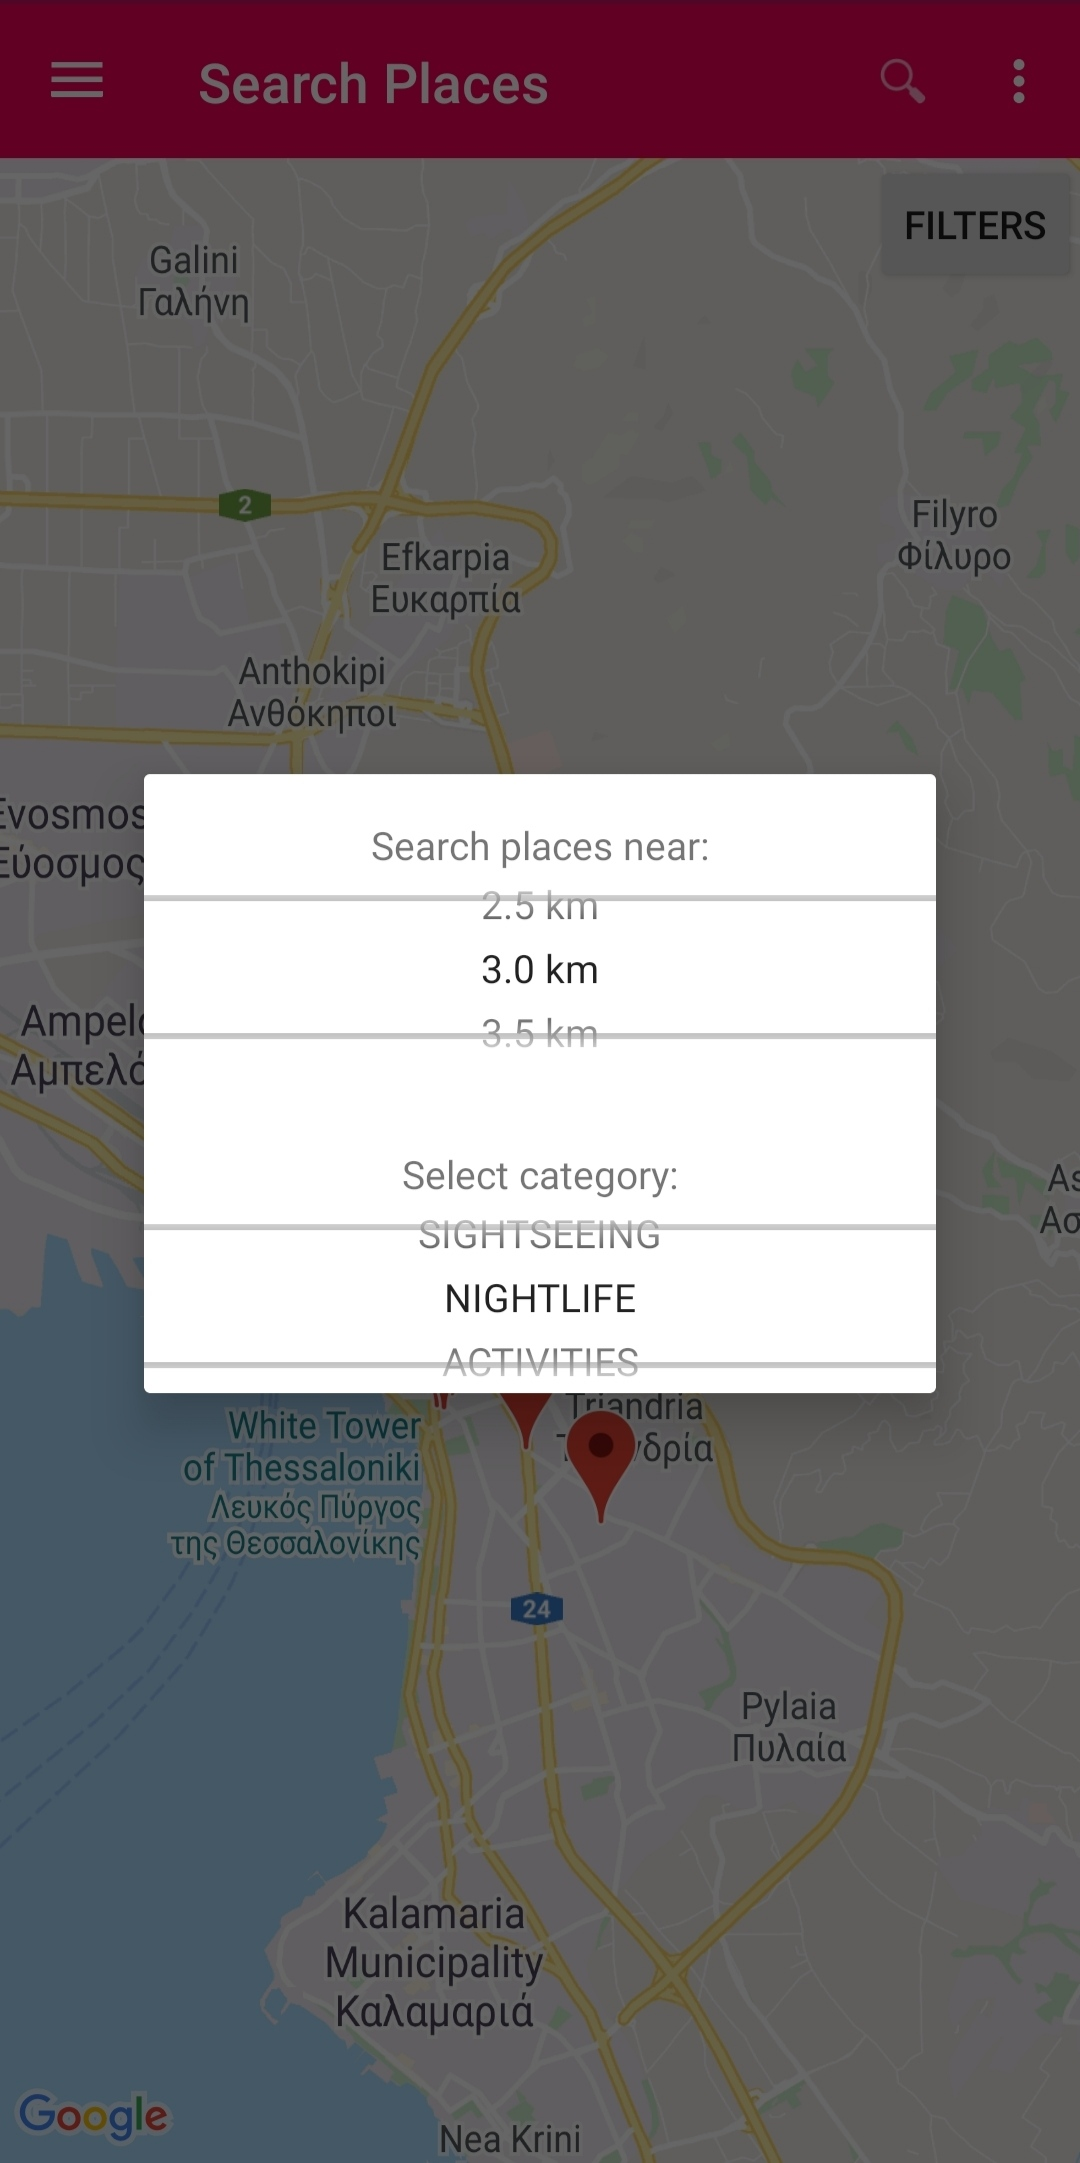
\includegraphics[scale=0.15]{images/search_places.jpg}
  \caption{\label{fig:search_places_1}Αναζήτηση τοποθεσιών σε ακτίνα 3 χιλιομέτρων για την κατηγορία της ``Νυχτερινής Ζωής''.}
\end{figure}

Στο διάγραμμα~\ref{fig:search_places_2} φαίνεται το αποτέλεσμα μιας 
αναζήτησης τοποθεσιών. Κατά την εύρεση των τοποθεσιών, για τη 
διευκόλυνση του χρήστη γίνεται μεγέθυνση στο χάρτη ώστε να φαίνονται 
όλες οι τοποθεσίες που πληρούν τα κριτήρια που τέθηκαν. Στα 
αποτελέσματα που βρέθηκαν, η κάθε τοποθεσία συμβολίζεται με ένα στίγμα
στο χάρτη. Μετά την εμφάνιση των αποτελεσμάτων, ο χρήστης πατώντας
πάνω σε ένα σημείο στο χάρτη, μπορεί να δει λεπτομέρειες όπως το όνομα
της τοποθεσίας. Επιπρόσθετα, ο χρήστης έχει τη δυνατότητα να λάβει 
οδηγίες από την εφαρμογή χαρτών της Google ώστε να επισκεφθεί την 
επιλεγμένη τοποθεσία.
\begin{figure}[h]
  \centering
  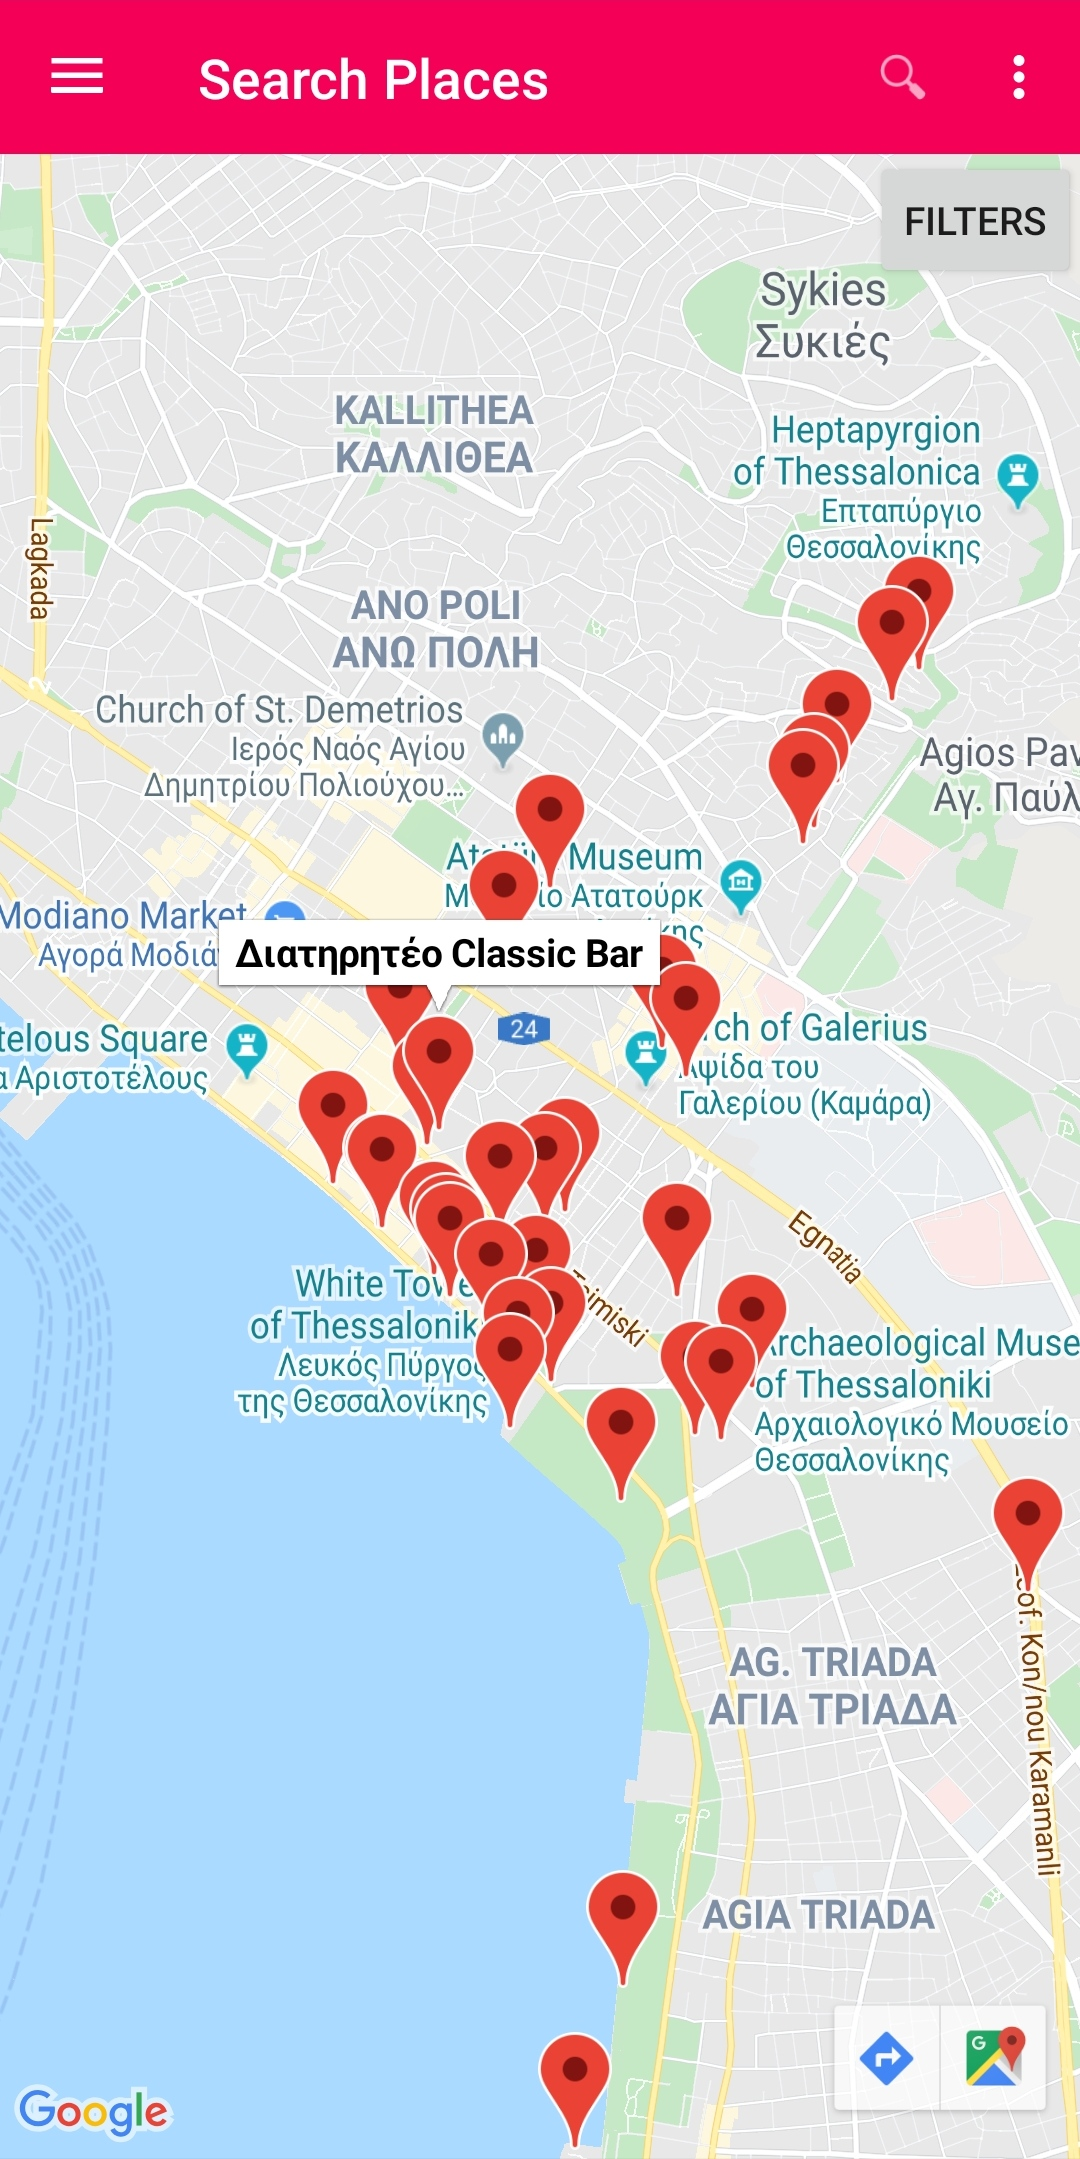
\includegraphics[scale=0.15]{images/search_places_result.jpg}
  \caption{\label{fig:search_places_2}Αποτέλεσμα αναζήτησης τοποθεσιών.}
\end{figure}

\subsection{Δημιουργία λογαριασμού χρήστη}
Όπως αναφέρθηκε προηγουμένως, κάποιες λειτουργίες της εφαρμογής 
απαιτούν από τον χρήστη να είναι συνδεδεμένος με τον λογαριασμό του. 
Έτσι και στην περίπτωση της ``Αναζήτησης τοποθεσιών'', εάν ο χρήστης 
επιλέξει να αναζητήσει τοποθεσίες χωρίς να είναι συνδεδεμένος, θα 
προβληθεί ένα μήνυμα που προτρέπει τον χρήστη να συνδεθεί ή να 
δημιουργήσει νέο λογαριασμό. Με την εμφάνιση του μηνύματος αυτού --- όπως φαίνεται και στο διάγραμμα \ref{fig:login_prompt} --- αποτρέπεται ο χρήστης στο να προβεί στη χρήση λειτουργιών που είναι διαθέσιμες μόνο για εγγεγραμμένους χρήστες.
\begin{figure}[h]
  \centering
  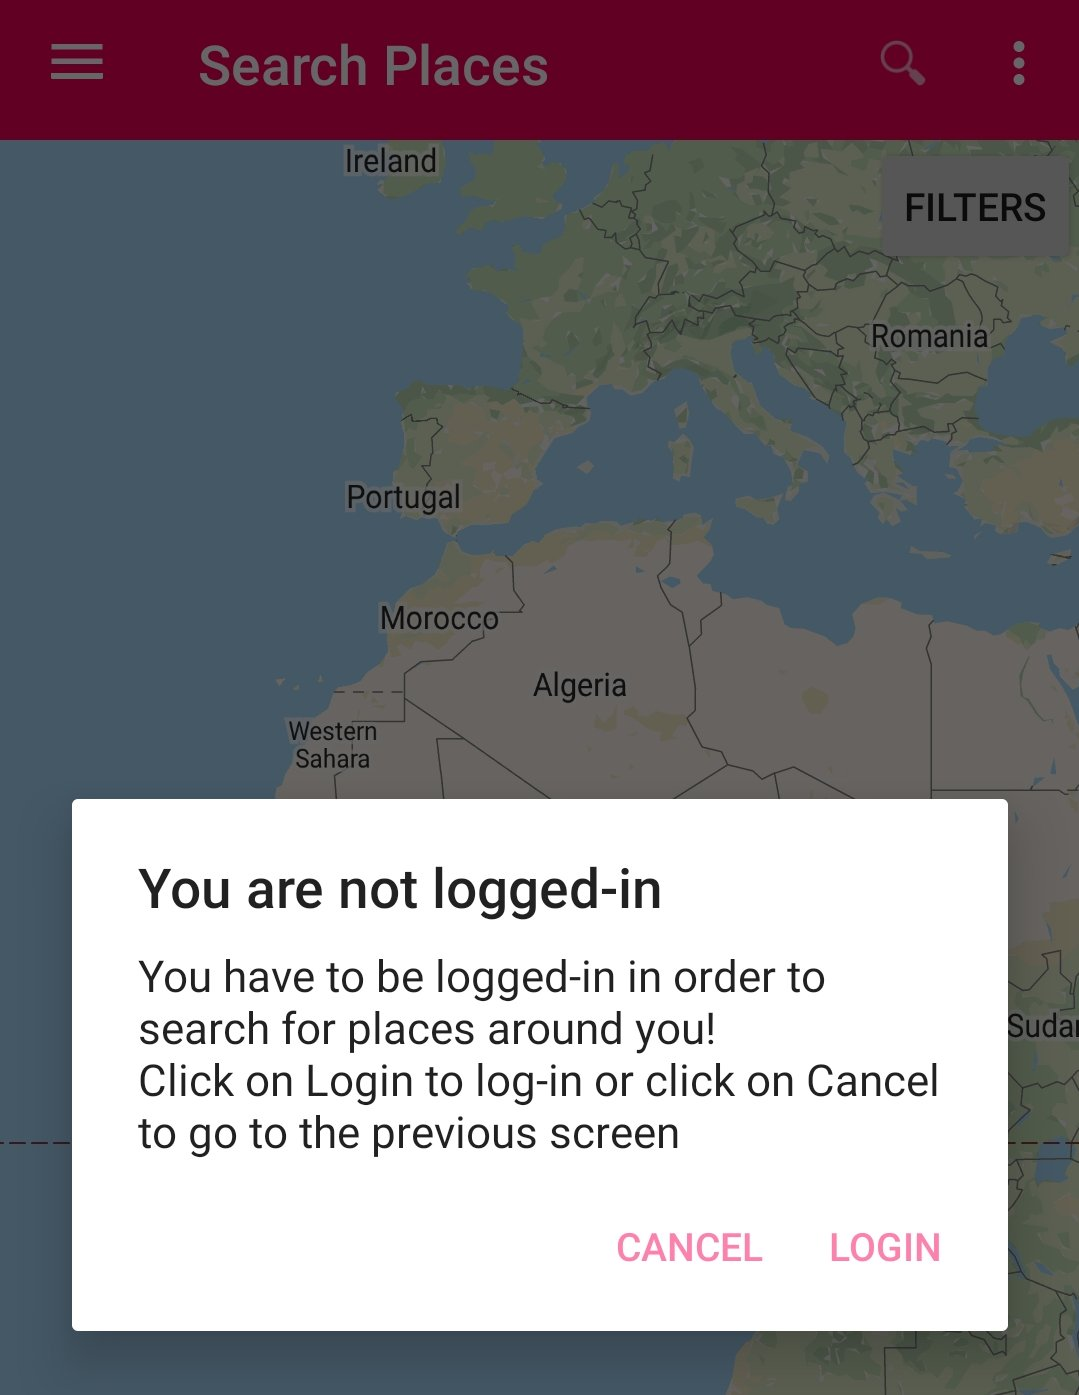
\includegraphics[scale=0.15]{images/login_prompt.jpg}
  \caption{\label{fig:login_prompt}Προτροπή του χρήστη σε σύνδεση με το λογαριασμό του.}
\end{figure}

\subsection{Διαχείριση ταξιδιών} \label{trip_management}
Μία ακόμα πολύ σημαντική λειτουργία της εφαρμογής είναι η δυνατότητα 
που παρέχεται στον χρήστη να δημιουργεί μελλοντικά ταξίδια, στα οποία 
αποθηκεύει τις τοποθεσίες που θέλει να επισκεφθεί.
Όπως φαίνεται στο διάγραμμα \ref{fig:future_trips} ο χρήστης έχει στη 
διάθεσή του τρεις καρτέλες ώστε να οργανώσει τα ταξίδια του.
Στην πρώτη καρτέλα προβάλλονται όλα τα μελλοντικά ταξίδια που έχει 
προγραμματίσει. Σε κάθε ταξίδι, ο χρήστης έχει την επιλογή να δει τις 
λεπτομέρειες του ταξιδιού, όπως για παράδειγμα ποιες τοποθεσίες έχει 
επιλέξει και κάποιες φωτογραφίες από τις τοποθεσίες αυτές. 
Επιπρόσθετα, υπάρχει η δυνατότητα να προβληθούν τα σημεία ενός ταξιδιού στον χάρτη.
\begin{figure}[h]
  \centering
  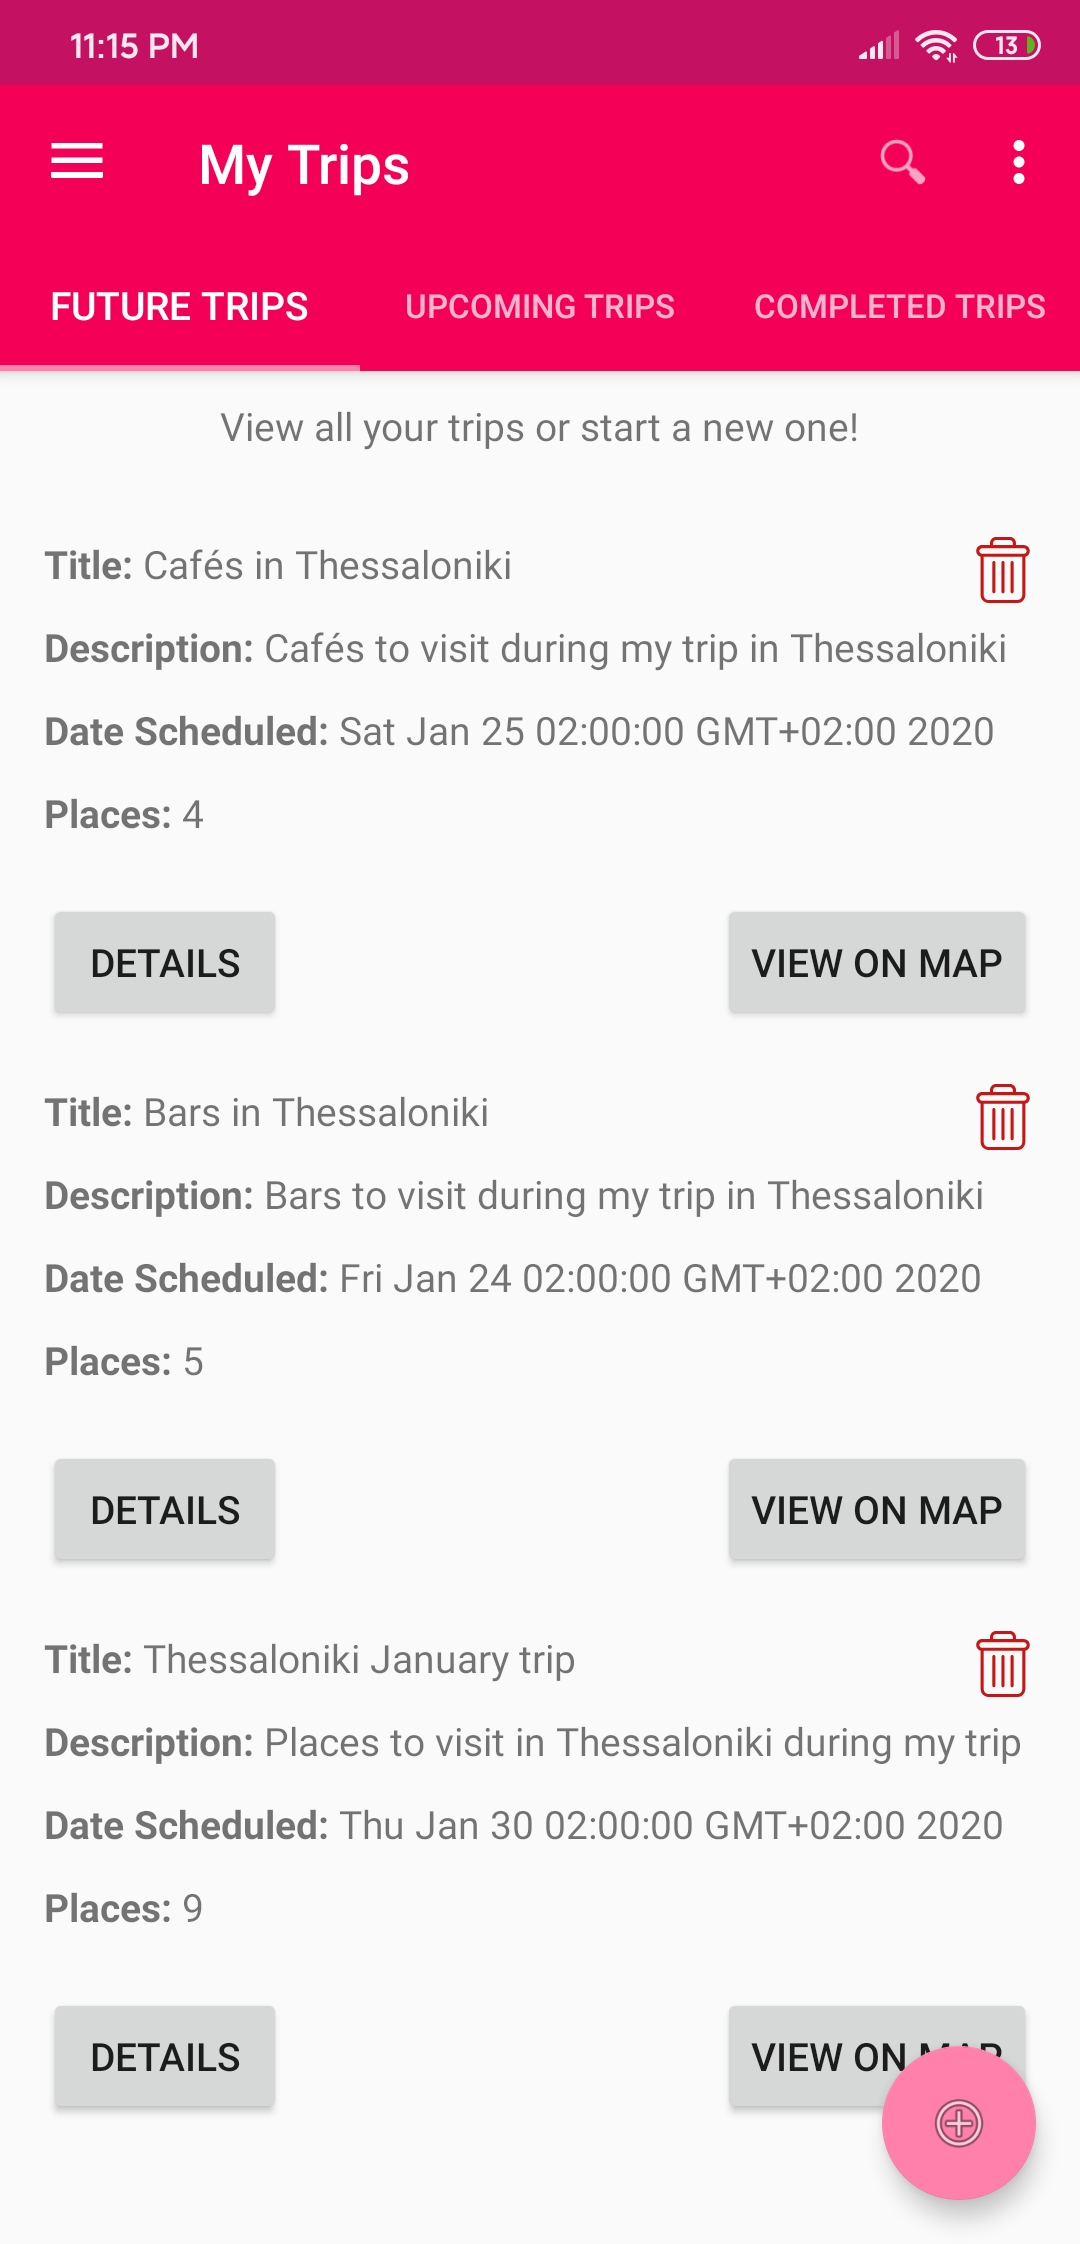
\includegraphics[scale=0.15]{images/future_trips.jpg}
  \caption{\label{fig:future_trips}Προβολή των μελλοντικών ταξιδιών}
\end{figure}

Στην δεύτερη καρτέλα, όπως απεικονίζεται και στο διάγραμμα \ref{fig:upcoming_trips} ο χρήστης μπορεί να διαχειριστεί τα ταξίδια του που πλησιάζουν, είναι δηλαδή προγραμματισμένα σε λιγότερο από μία εβδομάδα. Πάλι ο χρήστης, έχει τη δυνατότητα να δει τις λεπτομέρειες του ταξιδιού που πλησιάζει καθώς και να το δει στο χάρτη.
Σε αυτή την καρτέλα όμως υπάρχει και η πρόσθετη λειτουργία όπου ο χρήστης μπορεί να ξεκινήσει το ταξίδι του.
\begin{figure}[h]
  \centering
  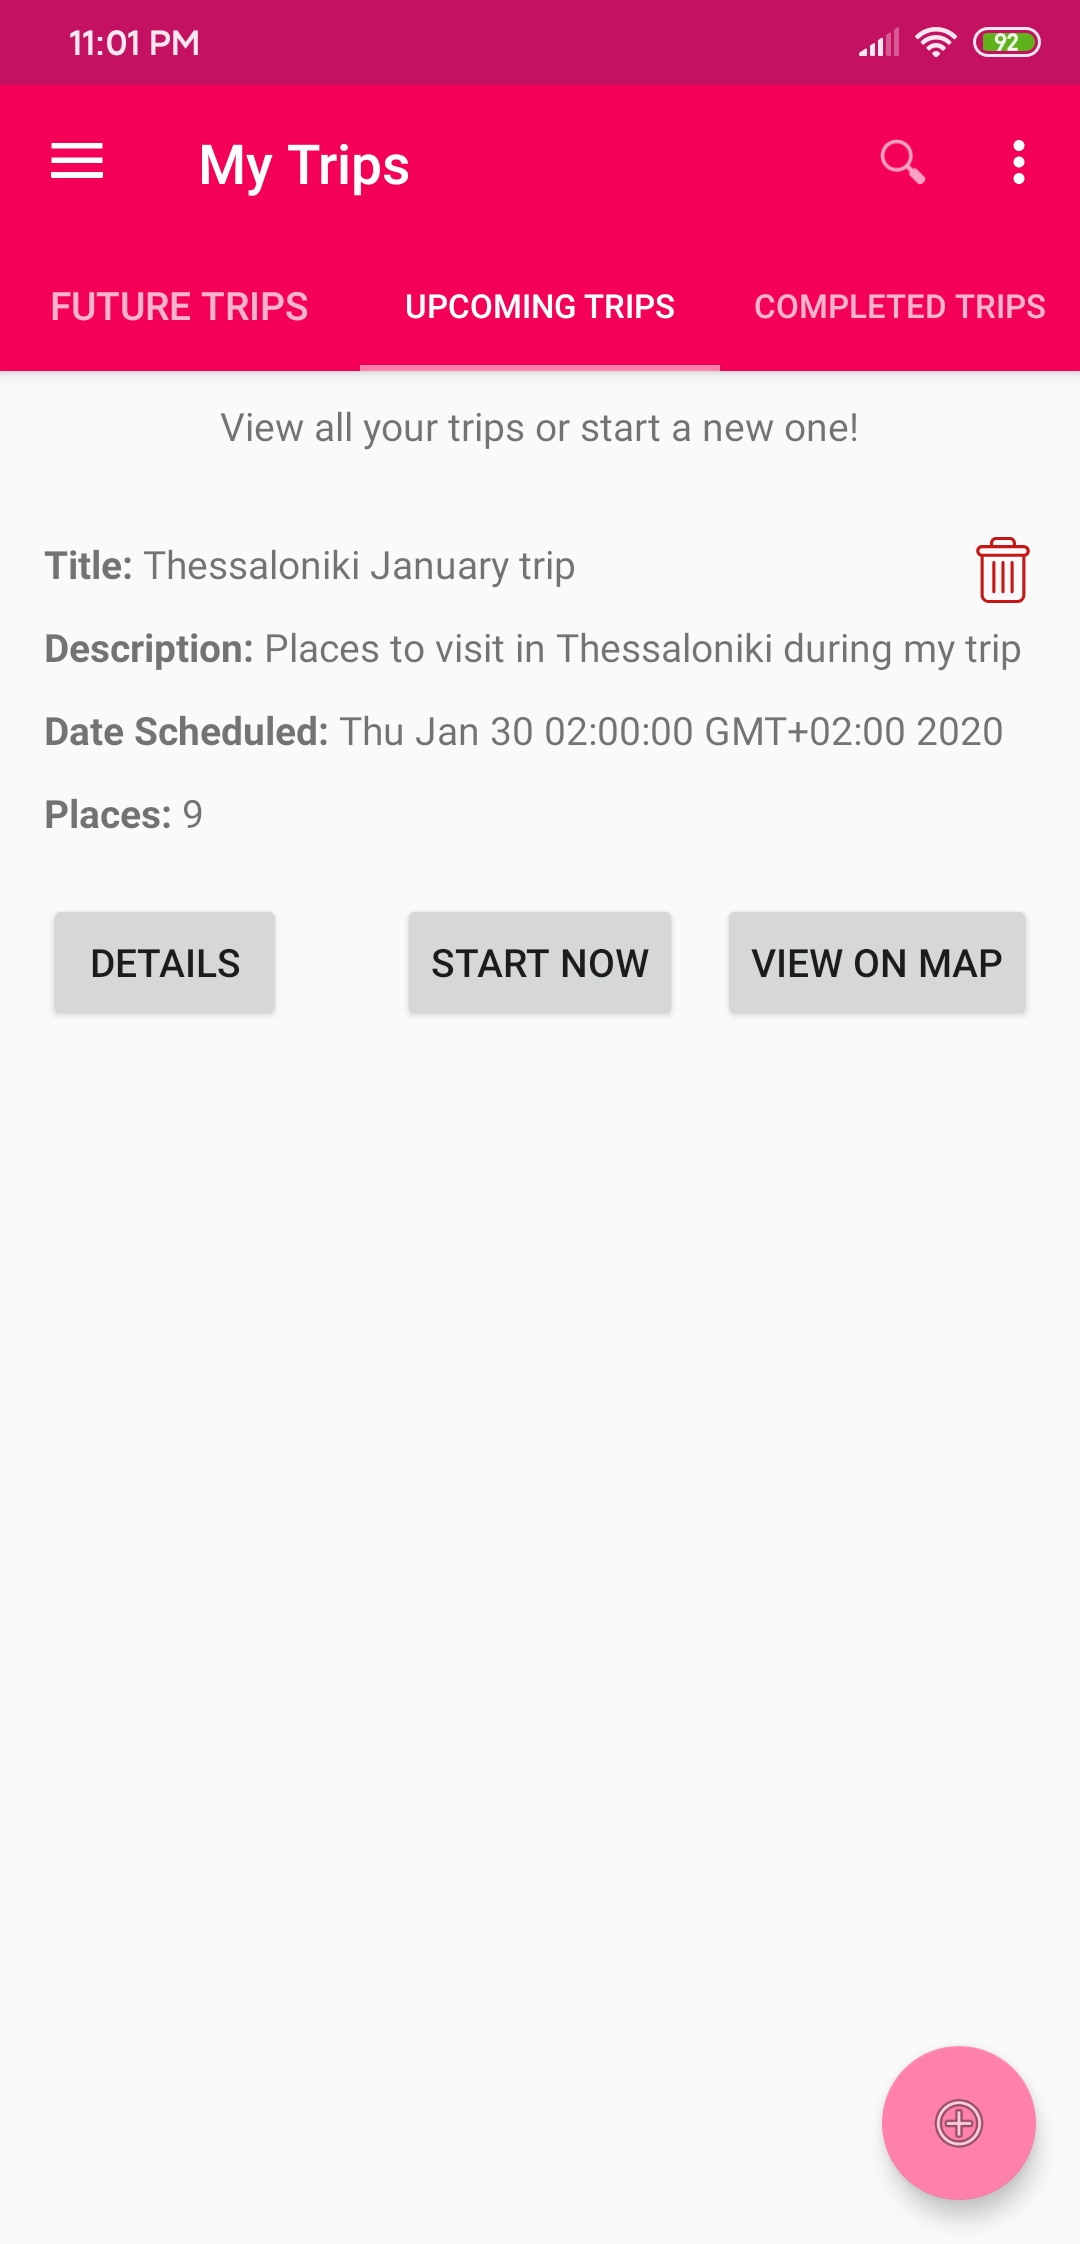
\includegraphics[scale=0.15]{images/upcoming_trips.jpg}
  \caption{\label{fig:upcoming_trips}Προβολή των επερχόμενων ταξιδιών που είναι προγραμματισμένα σε λιγότερο από μία εβδομάδα.}
\end{figure}

Πατώντας αυτή την επιλογή, εμφανίζεται ο χάρτης με τις τοποθεσίες που 
είχαν επιλεχθεί όπως στο διάγραμμα 
\ref{fig:upcoming_trips_directions}.
Στον χάρτη, η κάθε τοποθεσία εμφανίζεται με έναν αριθμό. Οι 
τοποθεσίες ταξινομούνται βάσει αλγορίθμου από την εφαρμογή του 
Server, όπου προτείνεται στο χρήστη η βέλτιστη διαδρομή που μπορεί να 
ακολουθήσει.
Κατά αυτόν τον τρόπο, η εφαρμογή προτείνει και σχεδιάζει στον χάρτη 
τη βέλτιστη διαδρομή που μπορεί να ακολουθήσει ο χρήστης, λαμβάνοντας φυσικά σαν παράμετρο τις τρέχουσες γεωγραφικές του συντεταγμένες.
\begin{figure}[H]
  \centering
  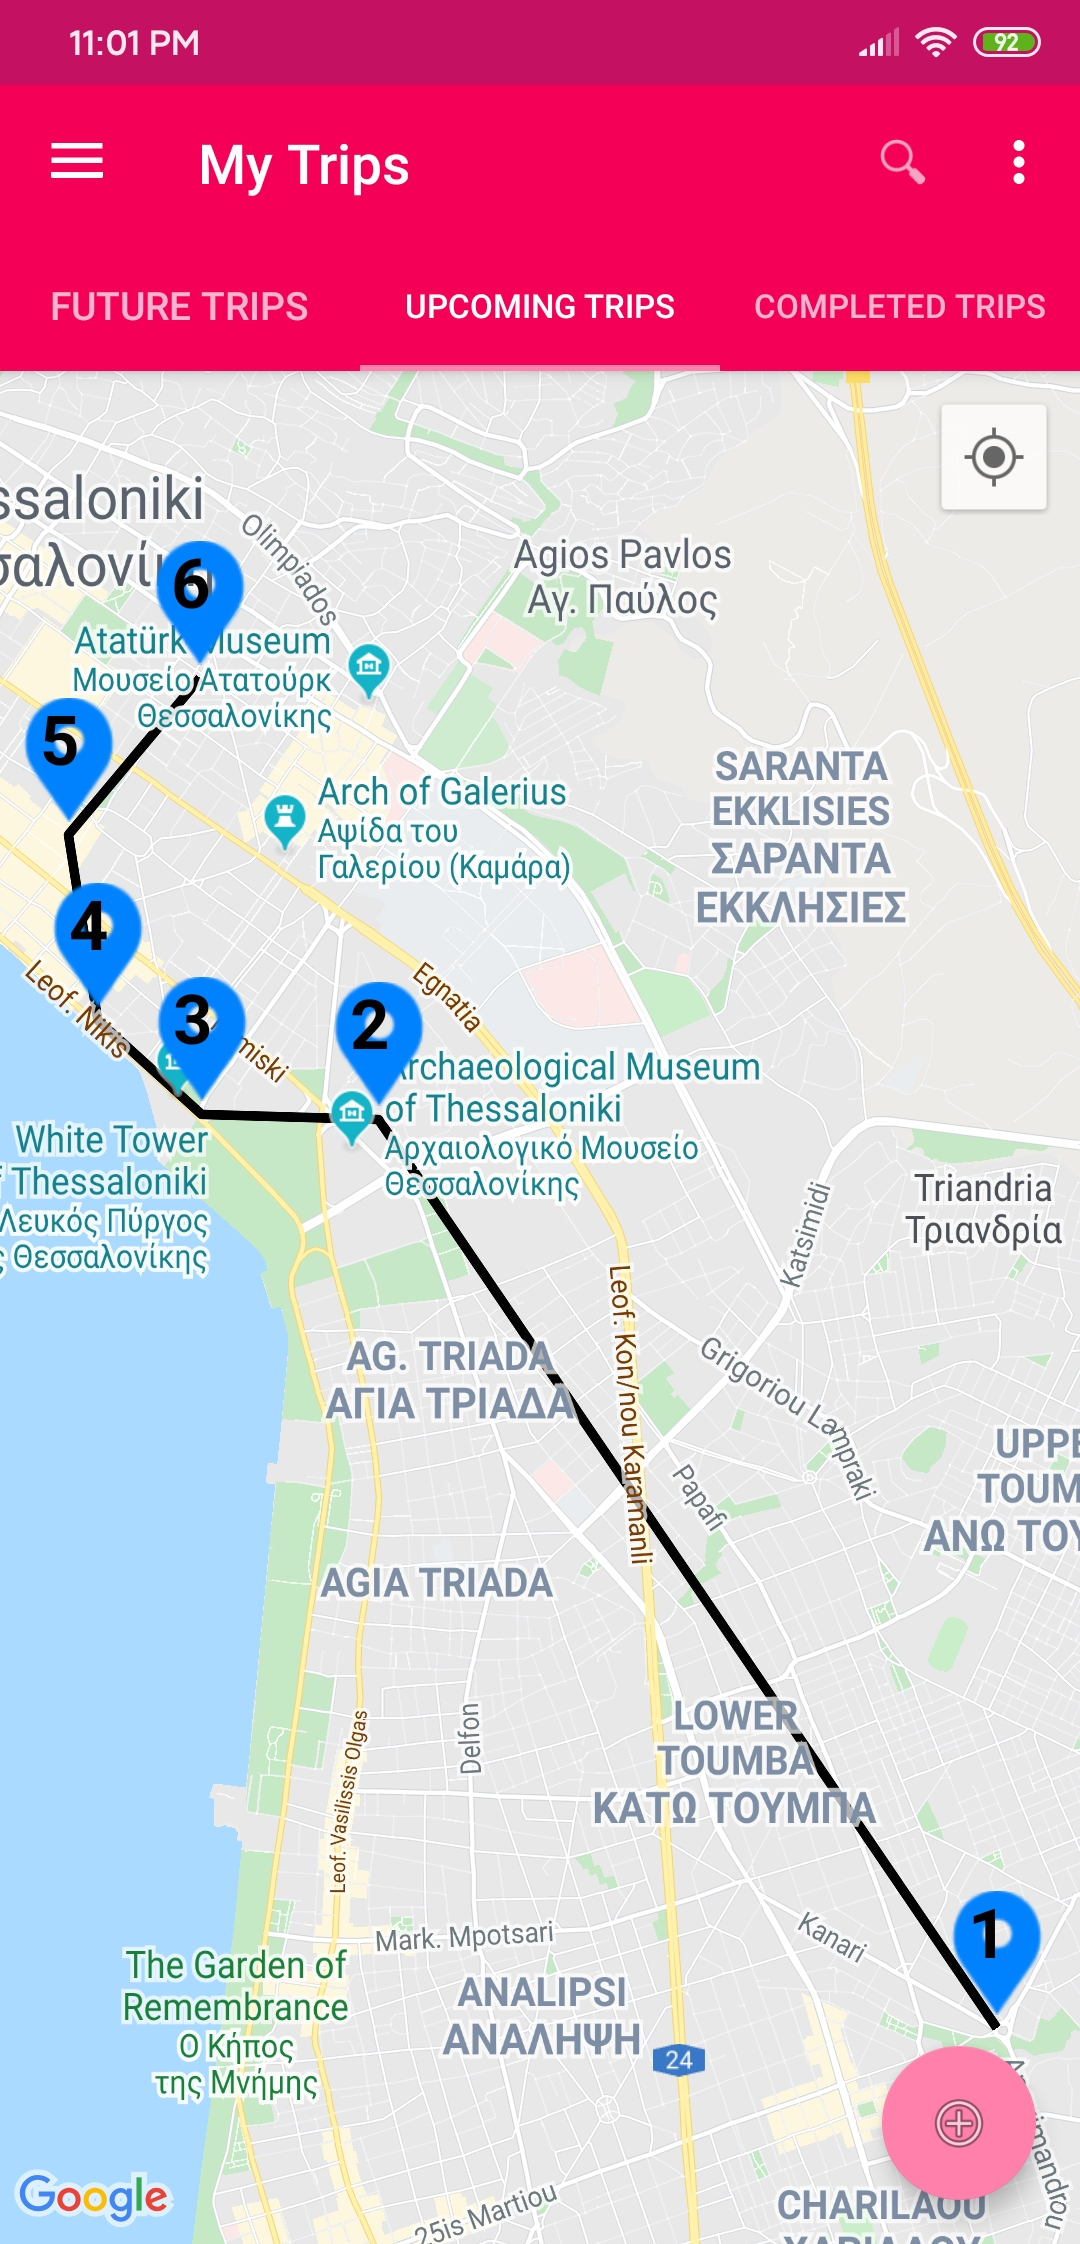
\includegraphics[scale=0.15]{images/upcoming_trips_directions.jpg}
  \caption{\label{fig:upcoming_trips_directions}Προβολή της προτεινόμενης διαδρομής των τοποθεσιών ενός ταξιδιού.}
\end{figure}

Αφότου τελειώσει ο χρήστης με το ταξίδι του, αυτό πλέον έχει μεταβεί 
στην κατάσταση του ``Ολοκληρωμένου ταξιδιού'' όποτε και πλέον μπορεί να 
βρεθεί μόνο στην τρίτη καρτέλα.
Σε αυτή την καρτέλα εμφανίζονται μόνο τα ταξίδια που έχουν ολοκληρωθεί 
και υπάρχουν κυρίως για να κρατάει ο χρήστης ιστορικό των ταξιδιών του 
αλλά και των τοποθεσιών που επισκέφθηκε σε αυτά.

\subsection{Οι Δέκα Δημοφιλέστερες τοποθεσίες}
Στο μενού της εφαρμογής, μεταξύ των άλλων λειτουργιών υπάρχει και αυτή 
στην οποία ο χρήστης έχει τη δυνατότητα να δει τις δέκα 
δημοφιλέστερες τοποθεσίες της πόλης του. Στον σχετικό χάρτη που εμφανίζεται, υπάρχουν δέκα σημεία με τις πιο δημοφιλείς τοποθεσίες που υπάρχουν 
στην πόλη που βρίσκεται ο χρήστης. Ο χρήστης, μπορεί να λάβει οδηγίες 
μέσω των χαρτών της Google ώστε να επισκεφθεί την κάθε τοποθεσία.

\subsection{Δημοφιλείς τοποθεσίες ανά εποχή του χρόνου} \label{popular_places_by_season_section}
Μία ακόμα ενδιαφέρουσα λειτουργία που είναι διαθέσιμη στην αρχική 
οθόνη της εφαρμογής, είναι η προβολή των πιο δημοφιλών τοποθεσιών για 
την τρέχουσα εποχή του χρόνου. Αυτή η λειτουργία είναι διαθέσιμη χωρίς να απαιτεί την ύπαρξη λογαριασμού χρήστη.
Κατά αυτό τον τρόπο, όπως απεικονίζεται και στο διάγραμμα \ref{fig:popular_season_places} προβάλλονται στον χρήστη οι 25 δημοφιλέστερες τοποθεσίες για την τρέχουσα εποχή του χρόνου και για την πόλη την οποία βρίσκεται ο χρήστης. Ο χρήστης, ``σέρνοντας'' την οθόνη με φορά προς τα δεξιά ή αριστερά, μπορεί να πλοηγηθεί ανάμεσα σε αυτές τις τοποθεσίες και να τις προσθέσει ενδεχομένως σε ένα επερχόμενο ταξίδι του.
\begin{figure}[h]
  \centering
  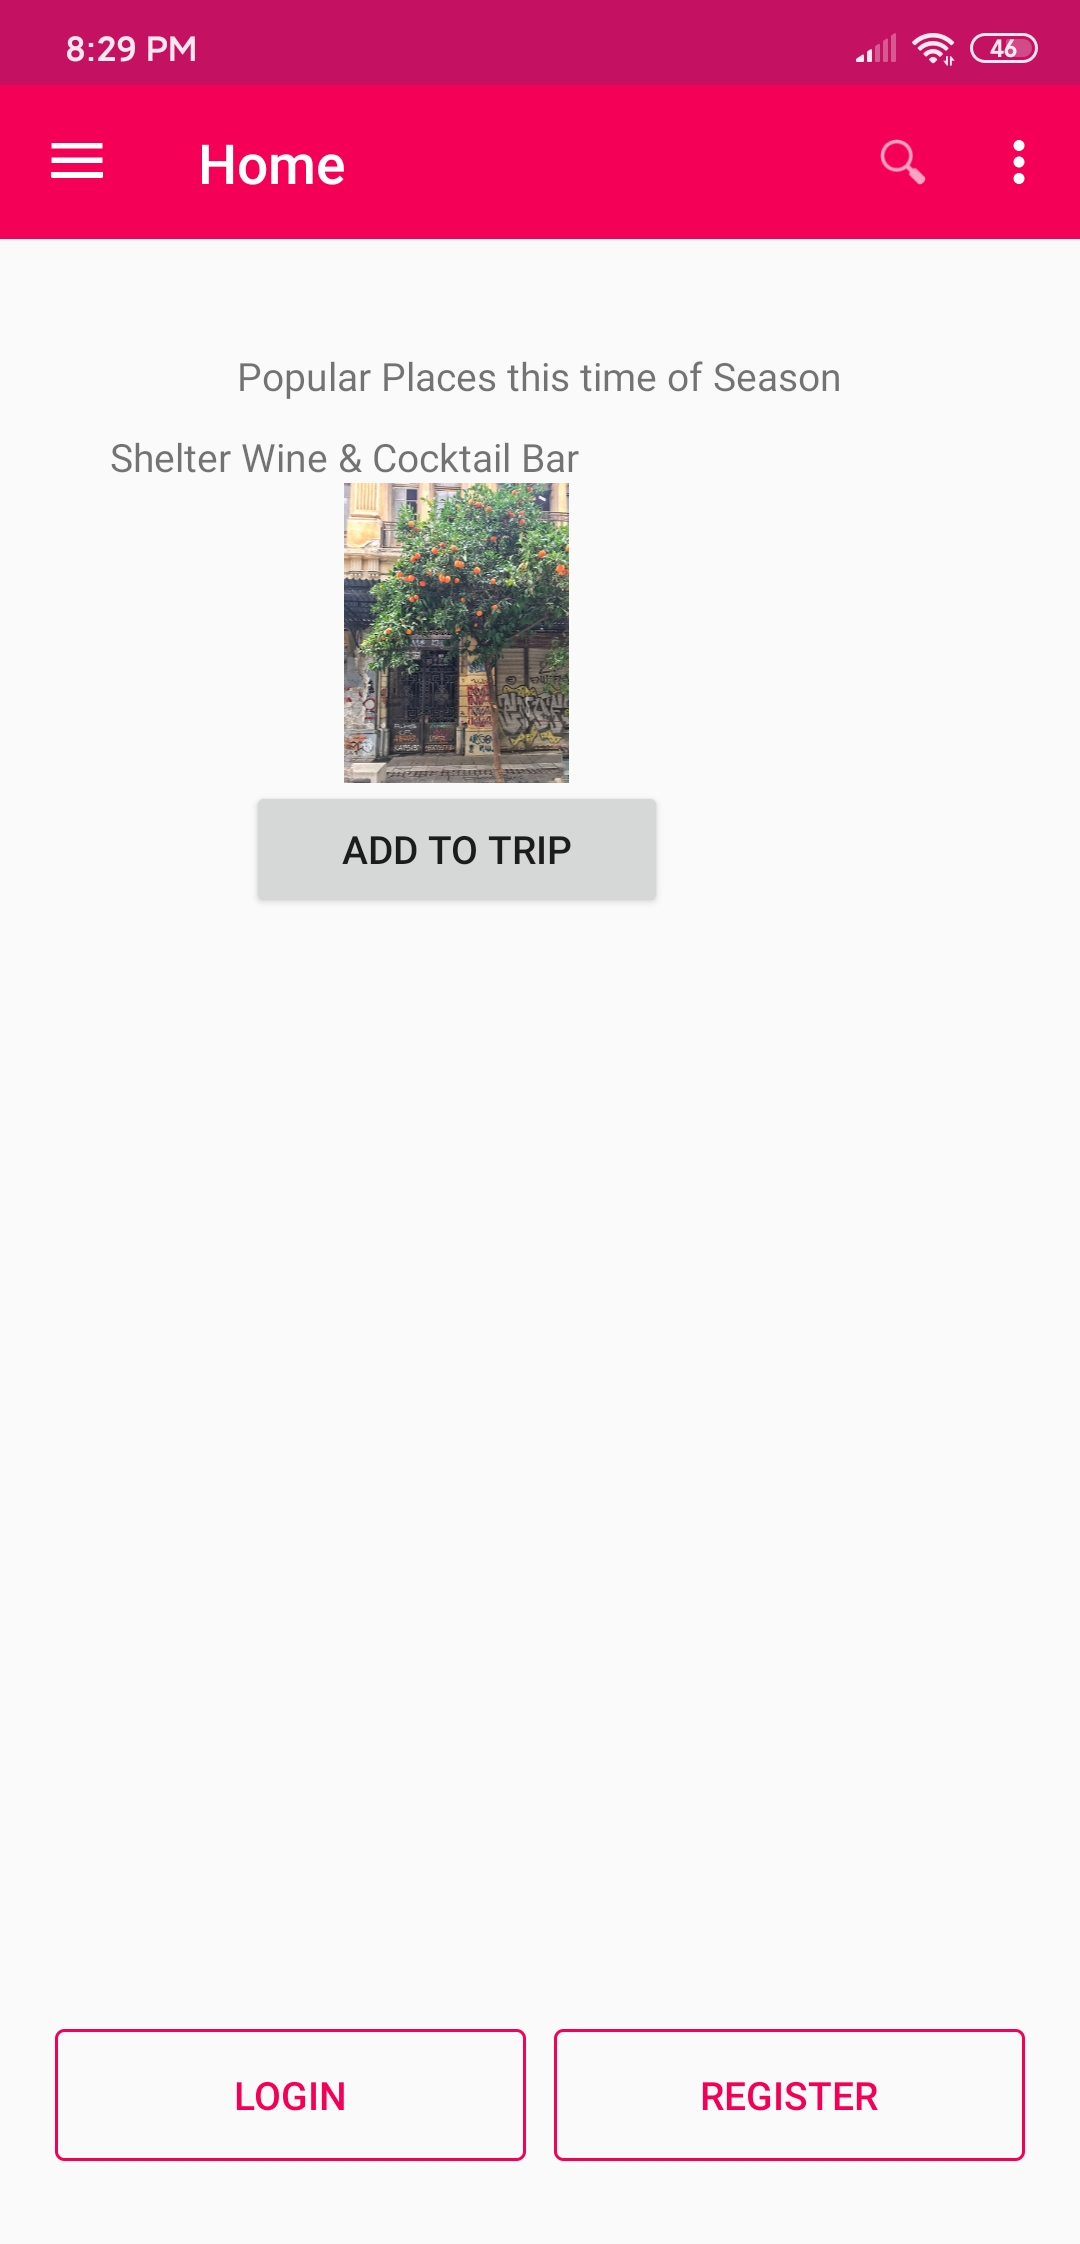
\includegraphics[scale=0.15]{images/popular_season_places.jpg}
  \caption{\label{fig:popular_season_places}Προβολή των δημοφιλών τοποθεσιών της πόλης που βρίσκεται ο χρήστης, για την τρέχουσα εποχή του χρόνου.}
\end{figure}

\subsection{Ενημέρωση χρήστη για τα επερχόμενα ταξίδια του} \label{sec:push_notification_upcoming_trip}
Πέραν των ταξιδιών που μπορεί να προγραμματίσει ο χρήστης, όπου προσθέτει τις τοποθεσίες που θέλει να επισκεφτεί, η εφαρμογή έχει τη δυνατότητα να ενημερώνει αυτόματα τον χρήστη για τα ταξίδια που έχει προγραμματίσει και πλησιάζουν. Πιο συγκεκριμένα, η εφαρμογή στέλνει push notification στις Android συσκευές των χρηστών, όταν για το ταξίδι που έχει προγραμματιστεί μένει λιγότερο από μία εβδομάδα. Επομένως, ο χρήστης λαμβάνει μία ειδοποίηση κάθε εικοσιτέσσερις (24) ώρες, ώστε να γίνει μία υπενθύμιση για το ταξίδι του.
Μία τέτοια ειδοποίηση φαίνεται στο διάγραμμα \ref{fig:push_notification}
\begin{figure}[h]
  \centering
  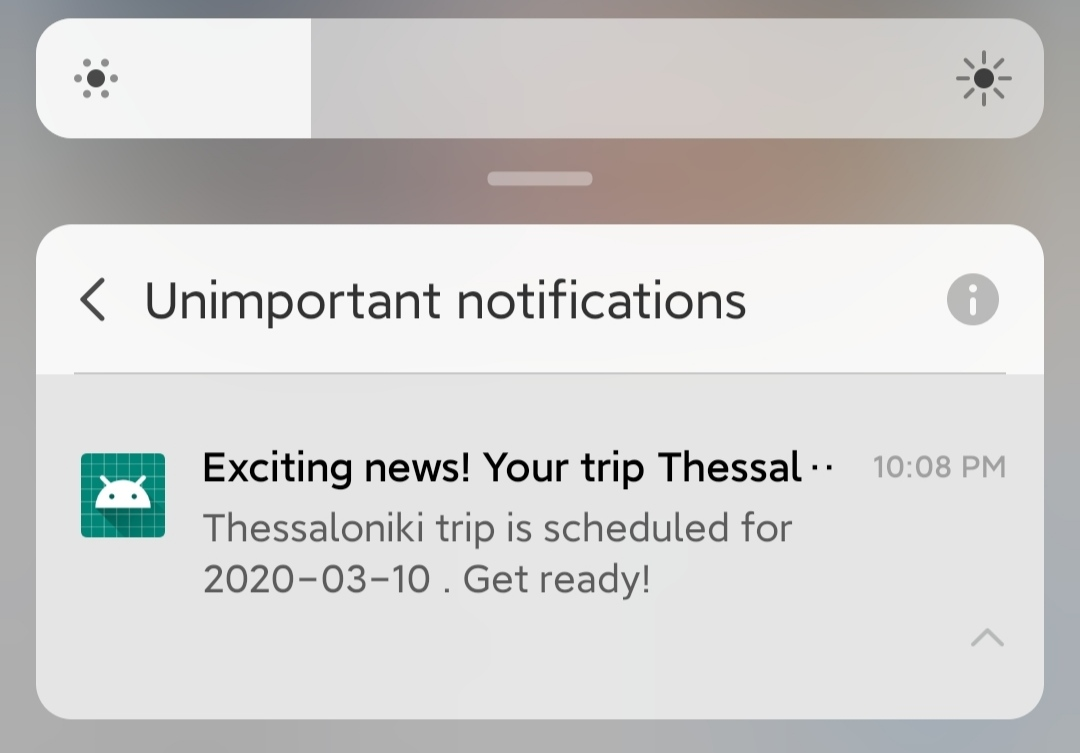
\includegraphics[scale=0.15]{images/push_notification.jpg}
  \caption{\label{fig:push_notification}Ειδοποίηση στην Android συσκευή του χρήστη, για ένα επερχόμενο ταξίδι}
\end{figure}

Στην ειδοποίηση, αναγράφεται η ημερομηνία για την οποία έχει προγραμματιστεί το ταξίδι, καθώς και το όνομα το οποίο έχει δώσει ο χρήστης στο ταξίδι του.

\chapter{Αρχιτεκτονική της εφαρμογής}
\section{Μοντέλο ανάπτυξης}
\subsection{Αρχικό μοντέλο ανάπτυξης}
Η βασική αρχή κατά την οποία δομήθηκε η εφαρμογή είναι το μοντέλο \textbf{Client-Server}.
Σε αυτό το μοντέλο, οι εργασίες και ο φόρτος εργασίας διανέμονται 
μεταξύ των παρόχων μιας υπηρεσίας ή ενός πόρου -που αποκαλούνται 
servers (εξυπηρετητές)- και των πελατών (clients) που κάνουν χρήση των 
παρεχόμενων υπηρεσιών.
Στο Trip Assistant, για τις ανάγκες του server (εξυπηρετητή), 
αναπτύχθηκε ένα REST API ώστε να παρέχει όλη τη λειτουργικότητα που 
χρειάστηκε για την εφαρμογή. Η ανάπτυξη του REST API έγινε με τη 
γλώσσα Java και τη χρήση του framework Spring. 
Αντίστοιχα, για την πλευρά του client αναπτύχθηκε μία εφαρμογή για 
συσκευές Android με τη γλώσσα Java, η οποία εφαρμογή εξυπηρετεί τις 
ανάγκες του τελικού χρήστη και γίνεται κατανάλωση του REST API που 
αναπτύχθηκε στην πλευρά του Server.

Στο παρακάτω διάγραμμα \ref{fig:base_architecture} βρίσκεται η αναπαράσταση της βασικής αρχιτεκτονικής που χρησιμοποιήθηκε για την υλοποίηση της εφαρμογής.

\tikzstyle{clientblock} = [rectangle, rounded corners, minimum width=2cm, minimum height=1cm,text centered, draw=black, fill=blue!40]
\tikzstyle{internetblock} = [cloud, minimum width=3cm, minimum height=1cm, text centered, draw=black, fill=red!30]
\tikzstyle{serverblock} = [rectangle, minimum width=4cm, minimum height=1cm, text centered, draw=black, fill=yellow!50]
\tikzstyle{clientarrow} = [thick,>=stealth]

\begin{figure}[h]
\begin{tikzpicture}[node distance=2cm]
    \node(client1) [clientblock] {Client};
    \node(client2) [clientblock, below of=client1] {Client};
    \node(client3) [clientblock, below of=client2] {Client};
    \node(internetcloud) [internetblock, right of=client2, xshift=2cm] {Internet}; 
    \node(webserver) [serverblock, text width=3cm, right of=internetcloud, xshift=2cm] {Trip-Assistant Web Server};
    \node[cylinder,draw=black,thick,aspect=0.3,minimum height=2cm,minimum width=1.5cm,shape border rotate=90,cylinder uses custom fill, cylinder body fill=red!30,cylinder end fill=red!10, right of=webserver, xshift=2cm] (database) {Database};
    
    \draw [clientarrow] (client1) -| (internetcloud);
    \draw [clientarrow] (client2) -- (internetcloud);
    \draw [clientarrow] (client3) -| (internetcloud);
    \draw [clientarrow] (internetcloud) -- (webserver);
    \draw [clientarrow] (webserver) -- (database);
\end{tikzpicture}
\caption{Αρχική αρχιτεκτονική ανάπτυξης του TripAssistant\label{fig:base_architecture}}
\end{figure}

Όπως φαίνεται και στην αρχιτεκτονική που περιγράφεται στο παραπάνω 
διάγραμμα, το κάθε τμήμα του συνόλου της εφαρμογής έχει ξεκάθαρο ρόλο ως προς τις αρμοδιότητες που έχει. Τον ρόλο των Client, έχει η εφαρμογή που αναπτύχθηκε για το Android, της οποίας ο σκοπός είναι να επικοινωνεί με τον Server μέσω του API που αναπτύχθηκε, ώστε να λαμβάνει τα δεδομένα που χρειάζεται για να κάνει προτάσεις τουριστικού περιεχομένου στο χρήστη.
Αντίστοιχα, το κομμάτι του server όπως φαίνεται αλληλεπιδρά με την βάση δεδομένων ώστε να αποθηκεύει αλλά και να διαβάζει τα δεδομένα που χρειάζεται. Έπειτα, τα δεδομένα αυτά παρέχονται στους Clients μέσω του API που αναπτύχθηκε και φιλοξενείται στο τμήμα του server.

\subsection{Εξέλιξη μοντέλου ανάπτυξης}
Το παραπάνω μοντέλο που περιγράφηκε, στην πορεία ενισχύθηκε προσθέτοντας ένα ενδιάμεσο λογισμικό για μερικές λειτουργίες της εφαρμογής. Αυτό το ενδιάμεσο λογισμικό διευκόλυνε την επικοινωνία μεταξύ του Client και του Server. Το ενδιάμεσο λογισμικό υλοποιήθηκε με το πρωτόκολλο Advanced Message Queuing Protocol (AMQP). Το πρωτόκολλο αυτό διευκολύνει την ανταλλαγή μηνυμάτων μεταξύ δύο μέσων, σε αυτή την περίπτωση του Client και του Server. Ωστόσο, υπήρξε μία περίπτωση χρήσης στην οποία το ενδιάμεσο λογισμικό χρησιμοποιήθηκε εξολοκλήρου στο λογισμικό που αναπτύχθηκε για τον Server. 

Ο λόγος που έγινε αυτό ήταν για να διαχωριστούν αλλά και να είναι ξεκάθαρες οι αρμοδιότητες που ανήκουν σε ένα τμήμα της εφαρμογής του Server. Επίσης με την προσθήκη αυτού του ενδιάμεσου λογισμικού, επιλύθηκε το πρόβλημα της εκτέλεσης χρονοβόρων εργασιών μέσω Internet. Παραδείγματος χάρη, ο Client χρειάστηκε να κάνει ένα HTTP request στον Server ώστε να ζητήσει τις πιο δημοφιλείς τοποθεσίες μίας πόλης για την τρέχουσα εποχή του χρόνου. Το συγκεκριμένο αίτημα, απαιτεί από τον Server την εκτέλεση χρονοβόρων διαδικασιών ώστε να συλλέξει τη δεδομένη στιγμή από την βάση δεδομένων τις δημοφιλέστερες τοποθεσίες για την πόλη που ζητήθηκε, έπειτα να τις χωρίσει βάσει εποχής και να κρατήσει τις 25 δημοφιλέστερες για την τρέχουσα εποχή του χρόνου. Η εκτέλεση αυτών των λειτουργιών θα μπορούσε να είναι αρκετά χρονοβόρα, γεγονός που θα μπορούσε να προκαλέσει ένα timeout στο HTTP request του Client προς τον Server. Χρησιμοποιώντας το πρωτόκολλο AMQP λύνεται αυτό το πρόβλημα. Ο client καταχωρεί ένα μήνυμα στο ενδιάμεσο λογισμικό ζητώντας τις δημοφιλέστερες τοποθεσίες για την τρέχουσα εποχή. Έπειτα, ο server ο οποίος ``ακούει'' την συγκεκριμένη ουρά, διαβάζει το μήνυμα και ξεκινάει τη διαδικασία του υπολογισμού των ζητούμενων δεδομένων. Όταν υπολογιστεί το αποτέλεσμα, ο Server καταχωρεί στο ενδιάμεσο λογισμικό ένα μήνυμα με το αποτέλεσμα που υπολόγισε, όπου ο Client ο οποίος ``ακούει'' σε αυτή την ουρά λαμβάνει το μήνυμα του αποτελέσματος και το επεξεργάζεται όπως χρειαστεί. Το συγκεκριμένο μοντέλο ονομάζεται που περιγράφηκε ονομάζεται Remote Procedure Call (RPC).

Η προσθήκη του ενδιάμεσου λογισμικού (middleware) στην αρχιτεκτονική του συστήματος αναπαρίσταται στο διάγραμμα \ref{fig:improved_architecture}.

\tikzstyle{twowayarrow} = [>=latex, <->, thick]
\tikzstyle{twowaygreenarrow} = [thick, >=latex,<->, blue]

\begin{figure}[h]
\begin{tikzpicture}[node distance=2cm]
    \node(client1) [clientblock] {Client};
    \node(client2) [clientblock, below of=client1] {Client};
    \node(client3) [clientblock, below of=client2] {Client};
    \node(internetcloud) [internetblock, right of=client2, xshift=2cm] {Internet}; 
    \node(webserver) [serverblock, text width=3cm, right of=internetcloud, xshift=2cm] {Trip-Assistant Web Server};
    \node(rabbitmqserver) [serverblock, text width=3cm, below of=webserver, yshift=-1.0cm] {RabbitMQ Server};
    \node[cylinder,draw=black,thick,aspect=0.3,minimum height=2cm,minimum width=1.5cm,shape border rotate=90,cylinder uses custom fill, cylinder body fill=red!30,cylinder end fill=red!10, right of=webserver, xshift=2cm] (database) {Database};
    
    \draw [clientarrow] (client1) -| (internetcloud);
    \draw [clientarrow] (client2) -- (internetcloud);
    \draw [clientarrow] (client3) -| (internetcloud);
    \draw [clientarrow] (internetcloud) -- (webserver);
    \draw [clientarrow] (webserver) -- (database);
    \draw [twowayarrow] (webserver) -- (rabbitmqserver);
    \draw [twowaygreenarrow] (client1) -- (2,-2) -- (2,-5) -- (rabbitmqserver);
    \draw [twowaygreenarrow] (client2) -- (2,-3) -- (2,-5) -- (rabbitmqserver);
    \draw [twowaygreenarrow] (client3) |- (rabbitmqserver);
\end{tikzpicture}
\caption{Η βελτιωμένη έκδοση της αρχιτεκτονικής του TripAssistant\label{fig:improved_architecture}}
\end{figure}

Όπως φαίνεται στο διάγραμμα, ο \textbf{Web Server} τροφοδοτεί τον \textbf{RabbitMQ Server} με μηνύματα τα οποία είτε προορίζονται για τον ίδιο, είτε για τους clients. Αντίστοιχα οι clients δέχονται μηνύματα από τον \textbf{RabbitMQ Server} τα οποία έχουν παραχθεί από τον \textbf{Web Server}. Ωστόσο, μόνο στην περίπτωση του RPC request που περιγράφηκε παραπάνω παράγουν μηνύματα με αποδέκτη τον \textbf{Web Server}.

Μία πιο λεπτομερής ανάλυση του συστήματος φαίνεται στο UML Component διάγραμμα \ref{fig:uml_component_diagram}. Στο διάγραμμα αυτό απεικονίζονται τα κύρια τμήματα της εφαρμογής και ο τρόπος με τον οποίο αλληλεπιδρούν ή εξαρτώνται μεταξύ τους.

\begin{figure}[h]
  \centering
  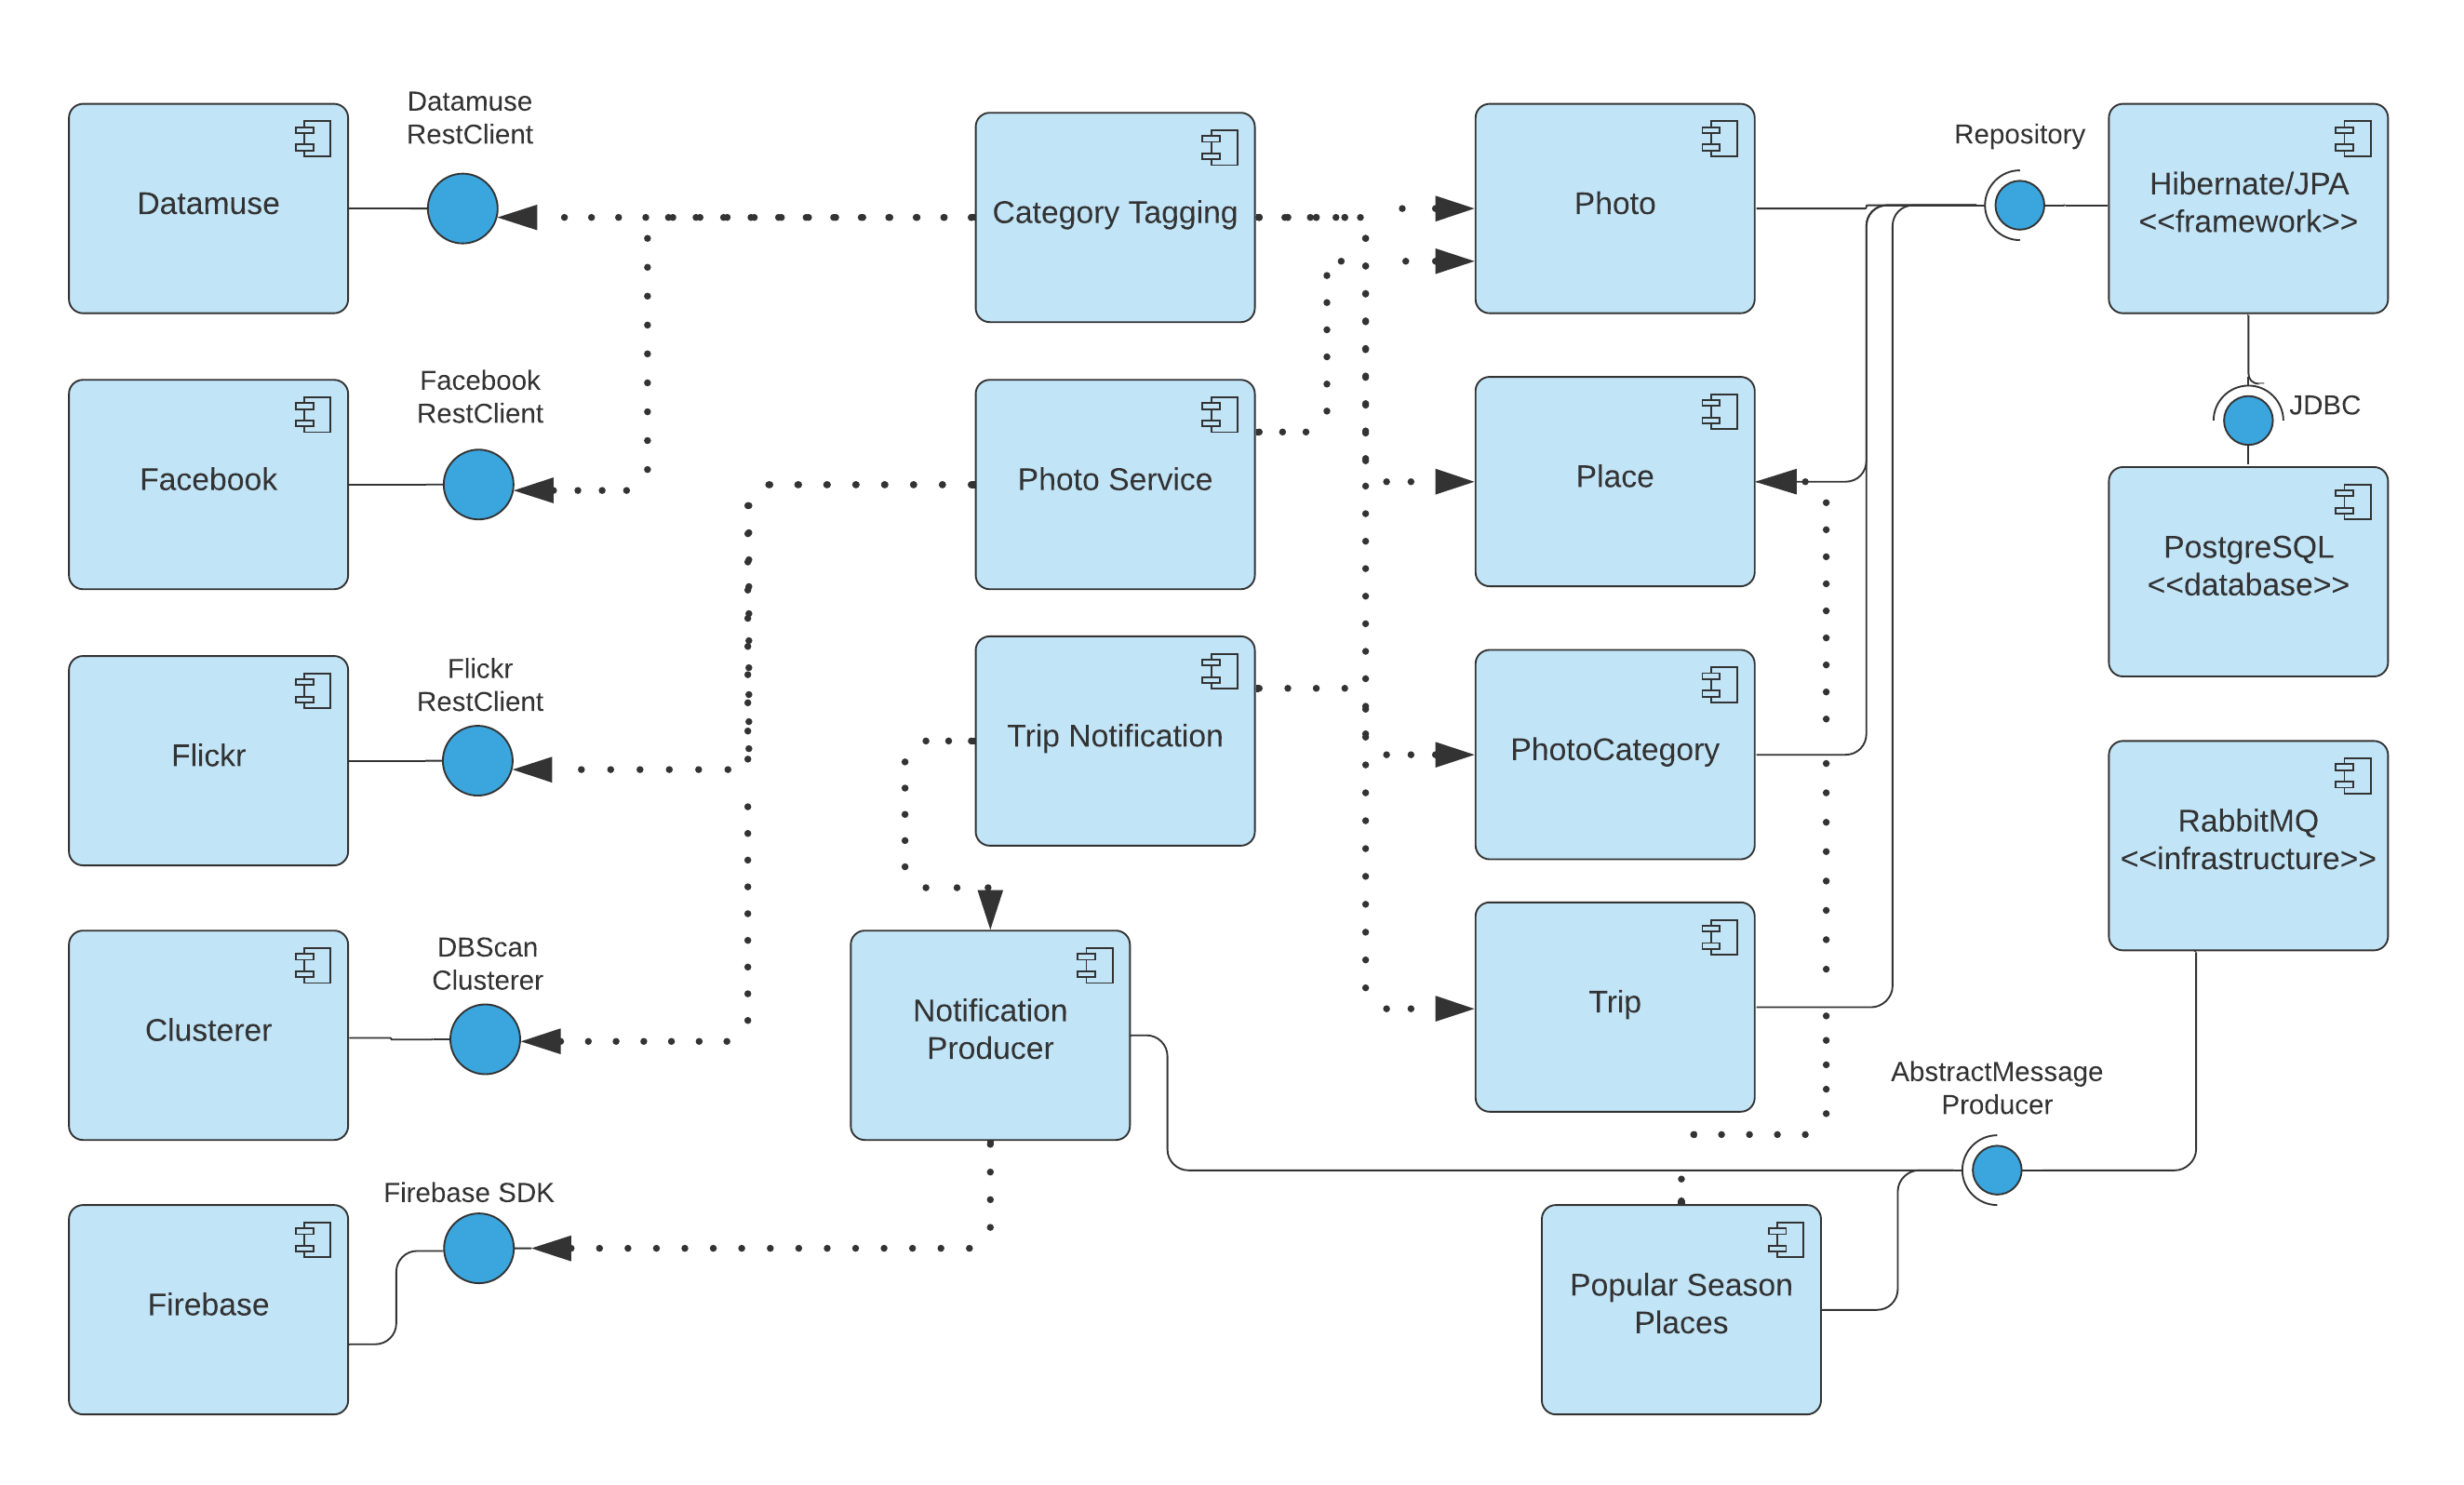
\includegraphics[scale=0.15]{images/uml_component_diagram.png}
  \caption{\label{fig:uml_component_diagram}UML Component Diagram του συστήματος}
\end{figure}

Παραδείγματος χάρη, φαίνεται πως για την υλοποίηση του Trip Notification χρησιμοποιήθηκε μία ουρά του RabbitMQ η οποία με τη σειρά της καλούσε την υπηρεσία του Firebase Cloud Messaging.

\section{Τεχνολογίες που χρησιμοποιήθηκαν}
Για την ανάπτυξη των δύο εφαρμογών (back-end και front-end) 
χρησιμοποιήθηκαν οι παρακάτω τεχνολογίες.

\subsection{Java} 
Η γλώσσα που χρησιμοποιήθηκε για την υλοποίηση του 
Web Server και της Android εφαρμογής που χρειάστηκαν για τις ανάγκες 
της πτυχιακής εργασίας είναι η Java. Η Java είναι μία 
αρκετά διαδεδομένη και δημοφιλής γλώσσα που χρησιμοποιείται ευρέως σε 
εφαρμογές διαφόρων μεγεθών. Επίσης, είναι cross-platform που σημαίνει 
πως μπορεί να τρέξει η εφαρμογή σε διαφορετικές πλατφόρμες και 
λειτουργικά χωρίς κάποια ιδιαίτερη παραμετροποίηση. Κατ' αυτό τον τρόπο, η εφαρμογή που αναπτύχθηκε για τον Server, έχει τη δυνατότητα να λειτουργήσει σε διάφορα λειτουργικά όπως το Unix αλλά και τα Windows.

\subsection{Android} Η εφαρμογή που αναπτύχθηκε για το κομμάτι του 
client ήταν μια εφαρμογή για Android κινητά. Το Android είναι ένα 
λογισμικό  ανοιχτού κώδικα, βασισμένο στο Linux το οποίο 
δημιουργήθηκε για ένα μεγάλο εύρος συσκευών. Επίσης, το σύνολο των 
λειτουργιών που παρέχει το λειτουργικό του Android, διατίθεται μέσω 
APIs γραμμένα στη γλώσσα προγραμματισμού Java~\cite{android_platform}.
Η ανάπτυξη εφαρμογών σε Android έχει το πλεονέκτημα πως έχει μικρό 
κόστος για τον εξοπλισμό και χρησιμοποιεί μεταξύ άλλων και την γλώσσα 
Java ή Kotlin όπως αναφέρθηκε και προηγουμένως. 
Στην εφαρμογή του Android Client που αναπτύχθηκε χρησιμοποιήθηκε η 
Java. Επίσης η διάθεση της εφαρμογής έχει αντίστοιχα ένα μικρό κόστος 
και είναι αρκετά εύκολη και άμεση η διαδικασία.

\subsection{Spring Boot Framework} Για την ανάπτυξη του REST API στην 
εφαρμογή του server χρησιμοποιήθηκε το Spring Framework.
Το Spring επιταχύνει και διευκολύνει την ανάπτυξη διαδικτυακών 
εφαρμογών, αφαιρώντας αρκετό από τον απαιτούμενο κώδικα για την 
παραμετροποίηση της εφαρμογής.
Με τη βοήθειά του Spring Boot υλοποιήθηκαν όλα τα endpoints του API που παρείχαν τις λειτουργίες δημιουργίας, 
διαβάσματος, ενημέρωσης και διαγραφής για κάθε πόρο του συστήματος 
(CRUD operations). Το Spring Boot, είναι βασισμένο στην αρχή 
convention over configuration, γεγονός που σημαίνει πως η ανάπτυξη 
ενός REST API είναι αρκετά γρήγορη, καθώς το Spring Boot παρέχει μία 
τυπική παραμετροποίηση για το σύστημα χωρίς να χρειάζεται ο 
προγραμματιστής να αφιερώσει πολύ χρόνο για την παραμετροποίηση.

\subsection{Hibernate Framework}
Για την διασύνδεση της εφαρμογής με τη βάση δεδομένων, χρησιμοποιήθηκε 
το Hibernate σε συνδυασμό με το Spring. Το Hibernate είναι ένα ORM 
(Object-Relational Mapping) Framework, το οποίο είναι μία υλοποίηση 
του  JPA (Java Persistence API) και συνεπώς μπορεί να χρησιμοποιηθεί 
σε οποιοδήποτε περιβάλλον υποστηρίζει το JPA συμπεριλαμβανομένων των 
Java SE (Standard Edition) και των JAVA EE (Enterprise Edition) 
εφαρμογών.
\cite{hibernate_orm}

\subsection{Spring Security}
Το Spring Security είναι ένα Framework που προσφέρει ένα επαρκώς 
παραμετροποιήσιμο σύστημα αυθεντικοποίησης/εξουσιοδότησης 
(authentication/authorization) και γενικότερα βοηθάει στην διαχείριση 
της πρόσβασης των χρηστών στις λειτουργίες της εφαρμογής. Το Spring 
Security είναι πλέον η συνήθης επιλογή για την ασφάλιση εφαρμογών 
βασισμένων στο Spring. Το Spring Security μεταξύ άλλων, προσφέρει 
προστασία από τις 10 μεγαλύτερες απειλές κατά τον οργανισμό OWASP όπως 
το Cross-Site Request Forgery (CSRF), Clickjacking.
\cite{spring_security}
Όπως αναφέρθηκε, για το authentication και το authorization των χρηστών στην εφαρμογή, χρησιμοποιήθηκε το Spring Security αλλά με την προσθήκη και χρήση των JWT (JSON Web Token). Στη συνέχεια, αφού υλοποιήθηκε το σύστημα ταυτοποίησης των χρηστών, ασφαλίστηκαν όλα τα endpoints της εφαρμογής του Server με το σύστημα αυτό.

\subsection{PostgreSQL (Βάση Δεδομένων)} Η εφαρμογή που αναπτύχθηκε είχε 
την ανάγκη να αποθηκευτούν δεδομένα για τους σκοπούς της καταχώρησης 
χρηστών αλλά και των δεδομένων των φωτογραφιών που στην πορεία 
επεξεργάζονταν. Για τους σκοπούς αυτούς, χρησιμοποιήθηκε η βάση 
δεδομένων PostgreSQL η οποία είναι μία σχεσιακή βάση δεδομένων 
ανοιχτού λογισμικού. Η αλληλεπίδραση με τη βάση δεδομένων γινόταν 
αποκλειστικά από την εφαρμογή του Server (back-end).

\subsection{RabbitMQ Message Broker} Μεταξύ των τεχνολογιών που 
χρησιμοποιήθηκαν είναι και ο Message Broker RabbitMQ. Το RabbitMQ είναι ένας 
message broker ανοιχτού λογισμικού το οποίο υλοποιεί διάφορα πρωτόκολλα μηνυμάτων, 
όπου στην συγκεκριμένη περίπτωση χρησιμοποιήθηκε το πρωτόκολλο AMQP. Υποστηρίζει 
διάφορες λειτουργίες όπως η δρομολόγηση μηνυμάτων σε ουρές, η επιβεβαίωση παράδοσης 
όπως και πολλά άλλα. Το RabbitMQ χρησιμοποιήθηκε σαν διαμεσολαβητής σε κάποιες από 
τις επικοινωνίες μεταξύ της εφαρμογής του Server και του Client. Μία περίπτωση που 
χρησιμοποιήθηκε ήταν για να διαχωρίσει (decouple) τις εργασίες σε ένα τμήμα του 
project. Μία άλλη περίπτωση ήταν η χρήση του για την εκτέλεση μιας χρονοβόρας 
διαδικασίας~\cite{rabbitmq_features}.

\subsection{Firebase Cloud Messaging} Το Firebase Cloud Messaging είναι 
μία υπηρεσία της Google, η οποία είναι μία cross-platform υπηρεσία που προσφέρει 
μία αξιόπιστη λύση για αποστολή μηνυμάτων χωρίς κόστος. Στην περίπτωση της 
εφαρμογής, χρησιμοποιήθηκε για να στέλνονται push notifications στην Android 
συσκευή των χρηστών ώστε να ειδοποιούνται για ταξίδια που έχουν προγραμματίσει μέσω 
της εφαρμογής και πλησιάζουν.

\subsection{JUnit} Το JUnit είναι ένα framework για που βοηθά στην 
σύνταξη unit tests και αναπτύχθηκε για την γλώσσα Java. Το JUnit 
χρησιμοποιήθηκε για να γραφτούν κάποια unit και integration tests στην 
εφαρμογή του Server ώστε να διασφαλιστεί η σωστή και απρόσκοπτη λειτουργία κάποιων 
τμημάτων της εφαρμογής.

\section{Διάγραμμα Κλάσεων UML}
Την περιγραφή και την ανάλυση της δομής του συστήματος, διευκολύνει το παρακάτω διάγραμμα κλάσεων σε UML. Στο διάγραμμα κλάσεων παρακάτω αναλύονται οι κλάσεις του συστήματος, οι ιδιότητές τους, οι λειτουργίες τους και η σχέση τους με άλλα αντικείμενα. 

\subsection{Περιγραφή UML διαγράμματος κλάσεων}
Γενικότερα, η UML είναι το στάνταρ πρότυπο που χρησιμοποιείται για την 
ανάλυση και σχεδίαση συστημάτων. Ένα από τα σημαντικότερα κομμάτια της 
UML είναι και τα διαγράμματα κλάσεων, τα οποία μοντελοποιούν την 
πληροφορία του τομέα ενδιαφέροντος σε αντικείμενα οργανωμένα σε 
κλάσεις καθορίζοντας και τις μεταξύ τους συσχετίσεις. Το κύριο κομμάτι 
ενός διαγράμματος κλάσεων είναι η κλάση η ίδια. Μία κλάση σε ένα UML 
διάγραμμα υποδηλώνει ένα σύνολο από αντικείμενα με κοινά 
χαρακτηριστικά. Μία κλάση αναπαρίσταται γραφικά από τετράγωνο 
χωρισμένο σε τρία μέρη. Το πρώτο μέρος περιέχει το όνομα της κλάσης το 
οποίο πρέπει να είναι μοναδικό σε ολόκληρο το διάγραμμα. Το δεύτερο 
μέρος περιέχει τις ιδιότητες μιας κλάσης συνοδευόμενες με το όνομά 
τους και τον τύπο τους. Το τρίτο μέρος περιέχει όλες τις λειτουργίες 
της κλάσης οι οποίες σχετίζονται με το αντικείμενο της κλάσης. Τέλος, 
αξίζει να σημειωθεί πως το δεύτερο και τρίτο μέρος είναι προαιρετικά.
Ένα παράδειγμα αναπαράστασης μιας κλάσης βρίσκεται στο διάγραμμα \ref{fig:uml_diagram_class}.
\begin{figure}[h]
\centering
\begin{tikzpicture}
    \umlclass{Person}{ 
        - age : int \\ -height : int \\ -weight : float \\ -name : String
    }{ 
        + setAge() \\ + setHeight()
    } 
\end{tikzpicture}
\caption{\label{fig:uml_diagram_class}Παράδειγμα UML Class}
\end{figure}

Οι συσχετίσεις σε ένα UML διάγραμμα είναι η σχέση μεταξύ δύο ή 
περισσότερων κλάσεων. Τα ονόματα των συσχετίσεων -όπως και τα ονόματα 
των κλάσεων- είναι μοναδικά μέσα σε ένα UML διάγραμμα. Η συσχέτιση 
μεταξύ δύο κλάσεων αναπαρίσταται γραφικά με μία γραμμή. Επίσης, η 
πολλαπλότητα σε μία συσχέτιση μεταξύ δύο κλάσεων C\textsubscript{1} 
και C\textsubscript{2} ορίζεται ως 
\textit{n\textsubscript{l}...n\textsubscript{u}}. Η πολλαπλότητα αυτή 
προσδιορίζει ότι κάθε αντικείμενο της κλάσης C\textsubscript{1} 
συμμετέχει το λιγότερο n\textsubscript{l} φορές και το πολύ 
n\textsubscript{u} φορές στη συσχέτιση. Όταν η πολλαπλότητα 
παραλείπεται, τότε εννοείται ότι είναι \textit{0\ldots*} δηλαδή μηδέν ή 
περισσότερες φορές. 

Τέλος, σημαντικό κομμάτι των UML διαγραμμάτων κλάσεων είναι η 
αναπαράσταση της κληρονομικότητας και των ιεραρχιών. Στην UML μπορεί να αναπαρασταθεί η κληρονομικότητα μεταξύ μίας γονικής κλάσης και μιας υποκλάσης. Κατά αυτό τον τρόπο, τα αντικείμενα της υποκλάσης κληρονομούν τις ιδιότητες της γονικής κλάσης έχοντας τις πρόσθετες ιδιότητες της εκάστοτε υποκλάσης~\cite{berardi2005reasoning}.

\subsection{UML διάγραμμα του TripAssistant}
\begin{figure}[H]
    \resizebox{0.7\textwidth}{\textwidth}{%
    \begin{tikzpicture}
        \umlclass[x=0, y=0]{Photo}{ 
            - id : Long \\ - title : String \\ - description : String \\ - latitude : String \\ - longitude : String \\ - url : String \\ - dateUploaded : Date \\ - rotation : int \\ - categories : List<PhotoCategory> 
        }{ }
        \umlclass[x=0, y=-8]{PhotoCategory}{ 
            - id : Long \\ - category : PhotoCategoryEnum \\ - photos : List<Photo> \\ - tags : List<String> 
        }{ }
        \umlclass[x=6, y=-3]{PhotoCategoryEnum}{ }{ + resolveCategory() }
        \umlunicompo[mult=1..*]{Photo}{PhotoCategory}
        \umlunicompo[mult=1..*]{PhotoCategory}{Photo}
        \umlunicompo[mult=1..1, geometry=-|]{PhotoCategory}{PhotoCategoryEnum}
        \umlclass[x=0, y=-16]{Place}{ 
            - id : Long \\ - title : String \\ - description : String \\ - latitude : String \\ - longitude : String \\ - city : City \\ - visits : int \\ - categories : List<PhotoCategory> \\ - photoUrls : List<String> 
        }{ + incrementVisits() \\ + addPhoto()}
        \umlunicompo[mult=1..*]{Place}{PhotoCategory}
        \umlclass[x=6, y=-11]{City}{ 
            - latitude : String \\ - longitude : String  
        }{ + getCityFromLatLon \\ - getCityDistancePredicate()}
        \umlunicompo[mult=1..1, geometry=-|]{Place}{City}
    \end{tikzpicture}
    }
    \caption{UML Διάγραμμα κλάσης της εφαρμογής TripAssistant - Τμήμα 1}
    \label{fig:uml_diagram_tripassistant_part1}
\end{figure}

\begin{figure}[H]
    \begin{tikzpicture}
        \umlclass[x=0, y=0]{Trip}{ 
            - id : Long \\ - title : String \\ - description : String \\ - user : User \\ - status : Status \\ - scheduledFor : Date \\ - lastNotified : Date \\ - places : List<Place>
        }{ + belongsToUser()}
        \umlclass[x=7, y=0, width=4ex]{Place}{ 
            - id : Long \\ - title : String \\ - description : String \\ - latitude : String \\ - longitude : String \\ - city : City \\ - visits : int \\ - categories : List<PhotoCategory> \\ - photoUrls : List<String> 
        }{ + incrementVisits() \\ + addPhoto()}
        \umlunicompo[mult=1..*]{Trip}{Place}
        \umlsimpleclass[x=0, y=6]{Status}
        \umlunicompo[mult=1..1]{Trip}{Status}
        \umlnest[color=red]{Trip}{Status}
        \umlclass[x=0, y=-9]{User}{ 
            - id : Long \\ - firstName : String \\ - lastName : String \\ - username : String \\ - password : String \\ - trips : List<Trip> \\ - deviceTokens : List<String> 
        }{ }
        \umlunicompo[mult=1..*, angle1=-90, angle2=-140]{User}{Trip}
        \umlunicompo[mult=1..1]{Trip}{User}
        \umlclass[x=7, y=-9]{UserNotification}{ 
            - id : Long \\ - title : String \\ - details : String \\ - dateSent : Date \\ - acked : boolean \\ - user : User \\ - trip : Trip \\ - notificationImage : byte[] 
        }{ }
        \umlunicompo[mult=1..1]{UserNotification}{User}
        \umlunicompo[mult=1..1]{UserNotification}{Trip}
    \end{tikzpicture}
    \caption{UML Διάγραμμα κλάσης της εφαρμογής TripAssistant - Τμήμα 2}
    \label{fig:uml_diagram_tripassistant_part2}
\end{figure}

\begin{figure}[H]
    \begin{tikzpicture}
        \umlclass[x=0, y=0]{PopularPlace}{ 
            - id : Long \\ - name : String \\ - latitude : String \\ - longitude : String \\ - timesMentioned : Integer
        }{ }
        \umlclass[x=5, y=0]{Seasons}{ 
            - months : int[] 
        }{ + getSeason() \\ + getCurrentSeason() \\ + isInCurrentSeason() }
        \umlclass[x=10, y=0]{UserCredentials}{ 
            - username : String \\ - password : String
        }{ }
    \end{tikzpicture}
    \caption{UML Διάγραμμα κλάσης της εφαρμογής TripAssistant - Τμήμα 3}
    \label{fig:uml_diagram_tripassistant_part3}
\end{figure}

\section{Τεχνική ανάλυση των Λειτουργιών του TripAssistant}
\subsection{Εξαγωγή των δέκα δημοφιλέστερων τοποθεσιών} \label{sec:tech_top_10_popular}
Η πρώτη λειτουργία που υλοποιήθηκε για την εφαρμογή TripAssistant 
ήταν η εξαγωγή των δέκα δημοφιλέστερων τοποθεσιών από την πόλη που 
βρίσκεται ο χρήστης. Αρχικά, η εφαρμογή υποστήριζε μόνο την πόλη της 
Θεσσαλονίκης, όποτε παίρνοντας αυτό το παράδειγμα, έπρεπε σε πρώτο 
στάδιο η εφαρμογή να αποθηκεύσει όλες τις φωτογραφίες που τραβήχτηκαν 
στην πόλη της Θεσσαλονίκης. 

Οπότε, υλοποιήθηκε ένα Thread του οποίου 
η αρμοδιότητα ήταν να ανακτά από το Flickr μέσω του API που παρέχει, 
τις φωτογραφίες που έχουν τραβηχτεί στην πόλη της Θεσσαλονίκης τα 
τελευταία τρία χρόνια. Το Thread αυτό έτρεχε μία φορά την ημέρα ώστε 
να ενημερώνεται η εφαρμογή με τις νεότερες φωτογραφίες.
Για την επικοινωνία με το API του Flickr, αναπτύχθηκε στην εφαρμογή του backend ένας Rest Client με τη βοήθεια των εργαλείων που 
παρέχει το Spring.  

Εν συνεχεία, αναπτύχθηκε ακόμα ένα Thread το οποίο έτρεχε και αυτό με 
τη σειρά του μία φορά την ημέρα και εξήγαγε τις δέκα δημοφιλέστερες 
τοποθεσίες μιας πόλης. Για να επιτευχθεί αυτό, χρησιμοποιήθηκε ο 
clustering αλγόριθμος DBSCAN. Δίνοντας στον DBSCAN ένα set απο σημεία 
(τα οποία αποτελούνταν από τις γεωγραφικές συντεταγμένες των 
φωτογραφιών), ο αλγόριθμος βγάζει κάποια cluster που το καθένα 
περιέχει τα σημεία αυτά. Έπειτα, παίρνοντας τα δέκα cluster με τα 
περισσότερα σημεία έχουμε στη διάθεσή μας και τις δέκα δημοφιλέστερες 
τοποθεσίες. Τέλος, οι τοποθεσίες αυτές αποθηκεύονται στη βάση 
δεδομένων στον πίνακα \textbf{PopularPlace}.

Στο παραπάνω πρόβλημα, χρησιμοποιήθηκε ο αλγόριθμος DBSCAN καθώς 
δημιουργεί τα cluster βάσει πυκνότητας, οπότε οι φωτογραφίες οι 
οποίες έχουν τραβηχτεί στο ίδιο ή σε πολύ κοντινό σημείο 
συμπεριλαμβάνονται σε ένα cluster καθώς είναι γειτονικές. Αντιθέτως, 
οι φωτογραφίες οι οποίες είναι διάσπαρτες και αραιές στο χάρτη, 
θεωρούνται θόρυβος και επομένως παραλείπονται από τα αποτελέσματα.

\subsection{Σύστημα σύνδεσης/εγγραφής χρήστη και authentication}
Όπως αναφέρθηκε σε προηγούμενες ενότητες, οι περισσότερες λειτουργίες 
της εφαρμογής απαιτούν την ύπαρξη ενός λογαριασμού χρήστη.
Για το λόγο αυτό, υλοποιήθηκε το σύστημα εγγραφής/σύνδεσης χρήστη με 
τη βοήθεια του \textbf{Spring Security}. 

Κατά αυτό τον τρόπο, οι χρήστες δημιουργούν το λογαριασμό τους όπου 
παρέχουν ένα όνομα χρήστη και τον κωδικό τους. Ο κωδικός πρόσβασης 
των χρηστών, για λόγους ασφαλείας δεν αποθηκεύεται σαν κείμενο στη 
βάση δεδομένων, αλλά δημιουργείται ένα SHA-1 hash του κωδικού 
πρόσβασης που παρείχε ο χρήστης. Αντίστοιχα, κατά τη σύνδεση του 
χρήστη, δημιουργείται ένα hash του κωδικού που παρείχε ο χρήστης και 
στην περίπτωση που ταιριάζει με το hash που υπάρχει στη βάση 
δεδομένων, η σύνδεση του χρήστη στο λογαριασμό του είναι επιτυχής. 

Επιπλέον, τα περισσότερα endpoints του Web Server είχαν ασφαλιστεί, 
οπότε ένας χρήστης σε κάθε request έπρεπε να παρέχει ένα 
authentication token ώστε να μπορέσει να ταυτοποιηθεί και να 
εξυπηρετηθεί. Ο χρήστης, προμηθεύεται το token αυτό κατά την επιτυχή εγγραφή ή σύνδεση του. Το JWT token αυτό ακολουθεί το πρότυπο \textit{RFC7519} και είναι έγκυρο για μία ώρα από τη στιγμή της έκδοσής του. Ο Android client, αποθηκεύει το token αυτό και το χρησιμοποιεί σε όλα τα REST calls που γίνονται προς το API του TripAssistant WebServer, εώς ότου να λήξει.

\subsection{Αναζήτηση τοποθεσιών βάσει κατηγορίας}\label{sec:search_places_by_category_tech_analysis}
Για την αναζήτηση τοποθεσιών υλοποιήθηκε ένα endpoint που χρησιμοποιήθηκε από την Android εφαρμογή. Το endpoint αυτό δέχεται τέσσερις παραμέτρους, οι πρώτες δύο αφορούν τις γεωγραφικές συντεταγμένες του χρήστη, η επόμενη το εύρος (ακτίνα) σε χιλιόμετρα μέχρι το οποίο θα βρίσκονται οι τοποθεσίες. Η τελευταία παράμετρος είναι η κατηγορία των τοποθεσιών.

Για την εύρεση των τοποθεσιών, αρχικά η εφαρμογή ελέγχει αν οι 
συντεταγμένες του χρήστη βρίσκονται σε κάποια από τις πόλεις που 
υποστηρίζει η εφαρμογή. Έπειτα αναζητούνται οι τοποθεσίες που 
βρίσκονται σε αυτή την πόλη. Τέλος, με τη χρήση της φόρμουλας 
Haversine συγκρίνεται η απόσταση της τοποθεσίας από τις 
συντεταγμένες του χρήστη και επιστρέφονται αυτές οι οποίες 
βρίσκονται μέσα στην ακτίνα που ζητήθηκε.

Η φόρμουλα Haversine είναι μία μέθοδος με την οποία υπολογίζεται η 
απόσταση δύο συντεταγμένων σε έναν δισδιάστατο χάρτη. Η απόσταση 
αυτή είναι η πραγματική απόσταση των σημείων καθώς λαμβάνεται 
υπόψιν η σφαιρική τριγωνομετρία της γης, ωστόσο δεν λαμβάνονται 
υπόψιν τα ύψη των βουνών και τα βάθη των πεδιάδων~\cite{alam2016implementation}.

Η απόσταση Haversine μεταξύ δύο γεωγραφικών σημείων ορίζεται από την παρακάτω εξίσωση~\cite{yoga2017implementation}:

\begin{multline} \label{eq:haversine_equation}
    D = 2R*\\
    arcsin\left(\sqrt{sin^2(\frac{Lat_1-Lat_2}{2})+cos(Lat_1)*cos(Lat_2)*sin^2(\frac{Long_1-Long_2}{2})}\right)
\end{multline}

Όπου \textbf{Lat} είναι το Latitude δηλαδή το γεωγραφικό πλάτος,
\textbf{Long} το Longitude δηλαδή το γεωγραφικό μήκος και
\textbf{R} είναι η ακτίνα της γης (χρησιμοποιήθηκε η τιμή \textit{6372.8} ώστε 
το αποτέλεσμα της απόστασης να είναι σε χιλιόμετρα).

\subsection{Κατηγοριοποίηση τοποθεσιών}\label{sec:location_categorization}
Όπως αναφέρθηκε στην ενότητα \ref{sec:search_places_by_category_tech_analysis}
η εφαρμογή προσφέρει τη δυνατότητα στο χρήστη να αναζητήσει τοποθεσίες βάσει κατηγορίας. Για να επιτευχθεί αυτό, η εφαρμογή έχει κατηγοριοποιήσει κάθε τοποθεσία που υπάρχει στη βάση δεδομένων.
Η διαδικασία της κατηγοριοποίησης ξεκίνησε προσθέτοντας κάποια tags/λέξεις κλειδιά για κάθε κατηγορία που υποστηρίζει η εφαρμογή

\subsubsection{Προσθήκη tags σε κάθε κατηγορία}
Για το σκοπό αυτό, δημιουργήθηκε μία λειτουργία η οποία πρόσθετε σε 
κάθε κατηγορία μία λίστα από λέξεις κλειδιά/tags.
Χρησιμοποιώντας το REST call που περιγράφηκε στην ενότητα 
\ref{sec:datamuse_api_call} αναζητήθηκαν λέξεις κλειδιά βάσει του 
ονόματος της κάθε κατηγορίας. Έπειτα τα αποτελέσματα που επέστρεψε 
το παραπάνω REST call σώζονταν στη λίστα με τα tags της κάθε 
κατηγορίας. Επίσης υπήρχαν και κάποια βασικά tags για κάθε 
κατηγορία που υπάρχουν στον πηγαίο κώδικα της εφαρμογής. Και αυτά με
τη σειρά τους προστίθενται στα tags της εκάστοτε κατηγορίας.
Τέλος, αξίζει να σημειωθεί πως αυτή η διαδικασία προσθήκης tags σε 
μία κατηγορία γίνεται μία φορά για κάθε κατηγορία.

\subsubsection{Προσθήκη κατηγοριών σε μία τοποθεσία}
Αφού έχουν δημιουργηθεί τα tags για κάθε κατηγορία, έπειτα γίνεται 
μία προσπάθεια κατηγοριοποίησης των τοποθεσιών που υπάρχουν στην 
εφαρμογή. 
Στην προσπάθεια αυτή, αρχικά δημιουργείται μία λίστα που αποτελείται από τις λέξεις που βρίσκονται στο όνομα και την περιγραφή 
της τοποθεσίας. Έπειτα, χρησιμοποιείται το REST call που 
περιγράφηκε στην ενότητα \ref{sec:facebook_graph_places_api} για να 
αναζητηθούν επιπλέον πληροφορίες για την εκάστοτε τοποθεσία από το 
Graph Places API του \textbf{Facebook}. Προστίθενται στην 
προηγούμενη λίστα οι λέξεις που περιλαμβάνονται στο όνομα και την 
περιγραφή από το αποτέλεσμα που επέστρεψε το API του Facebook. 
Επιπρόσθετα, κρατείται και η κατηγορία που επέστρεψε το Facebook 
για την εκάστοτε τοποθεσία. 

Τέλος, συγκρίνεται η λίστα με τις 
λέξεις που συλλέχθηκε για την εκάστοτε φωτογραφία με τα tags της 
κάθε κατηγορίας που υπάρχει στην εφαρμογή. Σε όποιες κατηγορίες 
υπάρχει κάποια συσχέτιση, καταχωρείται η κατηγορία με την οποία 
υπήρξε συσχέτιση στις κατηγορίες της τοποθεσίας.
Τέλος, ενημερώνεται η βάση δεδομένων με τις κατηγορίες που 
προστέθηκαν σε κάθε τοποθεσία. 

\subsection{Προβολή δημοφιλών τοποθεσιών ανά εποχή του χρόνου}
Όπως αναφέρθηκε και στην ενότητα \ref{popular_places_by_season_section} μία από τις λειτουργίες της 
εφαρμογής είναι η προβολή των δημοφιλών τοποθεσιών για την τρέχουσα 
εποχή του χρόνου.
Για την υλοποίηση αυτής της λειτουργίας, έγινε ένα RPC call από την 
εφαρμογή στον Server. 
Ο Server λαμβάνοντας τις γεωγραφικές συντεταγμένες, δημιουργεί μία 
λίστα με όλες τις φωτογραφίες που βρίσκονται σε ακτίνα 50 
χιλιομέτρων. 
Έπειτα, παίρνοντας την ημερομηνία που μεταφορτώθηκε στην εκάστοτε 
πλατφόρμα (όπως το Flickr) η κάθε φωτογραφία , κρατούνται οι 
φωτογραφίες οι οποίες μεταφορτώθηκαν την τρέχουσα εποχή του χρόνου. 
Έπειτα, αυτές οι φωτογραφίες αντιστοιχίζονται με τις τοποθεσίες που 
υπάρχουν στη βάση δεδομένων και τελικά επιστρέφονται στην Android 
εφαρμογή προς προβολή.

Για την υλοποίηση του RPC call, χρησιμοποιήθηκε στις πλευρές του 
Server και του Android client το RabbitMQ. 
Ο λόγος που χρησιμοποιήθηκε ένα RPC call αντί για ένα απλό HTTP 
request είναι πως όλη η διαδικασία εξαγωγής των τοποθεσιών που 
ζητήθηκαν είναι αρκετά χρονοβόρα. 
Αν είχε χρησιμοποιηθεί ένα HTTP request τότε θα ήταν αρκετά πιθανό με μεγάλο όγκο δεδομένων στη βάση να υπάρξει timeout στο request.

Η αρχιτεκτονική του RPC call που ακολουθήθηκε παρουσιάζεται στο διάγραμμα \ref{fig:rabbitmq_rpc_call}.
\begin{figure}[h]
    \centering
    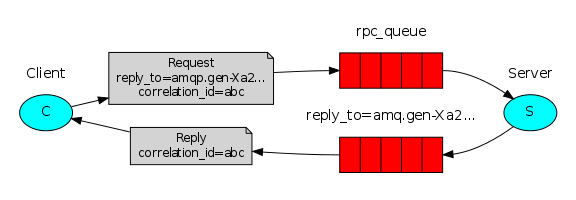
\includegraphics[width=\textwidth,height=\textheight,keepaspectratio]{images/rabbitmq_rpc_call.png}
    \caption{Αρχιτεκτονίκη ενός RPC call στο RabbitMQ}
    \label{fig:rabbitmq_rpc_call}
\end{figure}

Ο Client στην προκείμενη περίπτωση είναι η εφαρμογή Android η οποία κάνει ένα request σε ένα queue που είναι αφιερωμένο για την λειτουργία της εύρεσης τοποθεσιών για κάθε εποχή του χρόνου. 
Έπειτα στην εφαρμογή του Server τρέχει ένας worker ο οποίος ακούει στην προαναφερθείσα ουρά. 
Όταν λάβει ο Server το request, εκτελεί την χρονοβόρα εργασία της εύρεσης των τοποθεσιών για την τρέχουσα εποχή του χρόνου. 
Όταν ολοκληρωθεί αυτή η εργασία, στέλνει ένα μήνυμα με τα αποτελέσματα στο queue που είχε οριστεί στο \textbf{replyTo} του request του Client. 
Τέλος, ο Client ακούει στο queue που είχε οριστεί στο replyTo και λαμβάνει το αποτέλεσμα από τον Server. 
Τέλος, ο Client (η εφαρμογή Android) παρουσιάζει το αποτέλεσμα με τις τοποθεσίες στην αρχική σελίδα της εφαρμογής όπως φαίνεται και στο διάγραμμα \ref{fig:popular_season_places}.

\subsection{Έναρξη ταξιδιού χρήστη}\label{sec:start_user_trip}
Όπως παρουσιάστηκε και στην ενότητα \ref{trip_management}, μία πολύ ενδιαφέρουσα λειτουργία της εφαρμογής Android είναι η δυνατότητα των χρηστών να οργανώνουν τα ταξίδια τους.
Ανάμεσα στην οργάνωση των ταξιδιών, ο χρήστης έχει τη δυνατότητα να ξεκινήσει ένα ταξίδι που είχε οργανώσει. 
Ξεκινώντας ένα ταξίδι, η εφαρμογή προβάλλει στον χρήστη ένα χάρτη με τις τοποθεσίες οι οποίες είναι αριθμημένες. 
Αυτό αναπαρίσταται στο διάγραμμα \ref{fig:upcoming_trips_directions}. 
Η εφαρμογή προτείνει τη βέλτιστη διαδρομή που μπορεί να ακολουθήσει ο χρήστης, εξ ου και η αρίθμηση στις τοποθεσίες.

Για την εύρεση της βέλτιστης διαδρομής, αναπτύχθηκε ένας απλός αλγόριθμος στην εφαρμογή του backend. Ο αλγόριθμος αυτός παίρνει τη λίστα με τις τοποθεσίες και το σημείο εκκίνησης. Αρχικά ξεκινάει συγκρίνοντας την απόσταση του σημείου εκκίνησης από όλα τα υπόλοιπα σημεία. Παίρνει το σημείο με την μικρότερη απόσταση και το προσθέτει στη λίστα της διαδρομής. Έπειτα συγκρίνει την απόσταση του τελευταίου σημείου της διαδρομής με τα υπόλοιπα που μένουν και διαλέγει πάλι αυτό με τη μικρότερη απόσταση το οποίο το προσθέτει στη λίστα της διαδρομής που θα ακολουθηθεί. Κάθε φορά που προστίθεται ένα σημείο στη λίστα των σημείων της προτεινόμενης διαδρομής, τότε αφαιρείται από τη λίστα με τα σημεία. Αυτή η διαδικασία εκτελείται έως ότου η λίστα με τα σημεία μείνει κενή.

Παρακάτω βρίσκεται η υλοποίηση του αλγορίθμου που περιγράφηκε και έγινε στη γλώσσα Java.
 \lstset{frame=tb,
    tabsize = 4, 
    showstringspaces = false, 
    numbers = left, 
    commentstyle = \color{green}, 
    keywordstyle = \color{blue}, 
    stringstyle = \color{red}, 
    rulecolor = \color{black}, 
    basicstyle = \small \ttfamily , 
    breaklines = true, 
    numberstyle = \tiny,
}
\lstinputlisting[language = Java , label=shortestPathAlg, frame = trBL , firstnumber = last , escapeinside={(*@}{@*)}]{snippets/shortest_places_path.java}

Όπως φαίνεται και στον αλγόριθμο, η μέθοδος δέχεται μία λίστα με τα σημεία και ένα σημείο εκκίνησης και επιστρέφει τη λίστα ταξινομημένη βάσει της βέλτιστης διαδρομής. Οπότε, η εφαρμογή του Android παίρνει αυτή την ταξινομημένη λίστα και αριθμεί τα σημεία της λίστας στο χάρτη.
Επίσης και σε αυτή την περίπτωση, για την εύρεση της απόστασης μεταξύ 2 σημείων χρησιμοποιείται η φόρμουλα haversine \ref{eq:haversine_equation} που περιγράφηκε παραπάνω.

\subsection{Αποστολή push notifications στον χρήστη}
Στην ενότητα \ref{sec:push_notification_upcoming_trip} αναφέρθηκε η 
λειτουργία της αποστολής push notifications στην συσκευή Android του 
χρήστη. Για την αποστολή των push notifications, χρησιμοποιήθηκε το 
Firebase Cloud Messaging, μία υπηρεσία της Google.

Πιο συγκεκριμένα, στην εφαρμογή του back-end αναπτύχθηκε ένα Thread 
το οποίο κάθε δώδεκα ώρες αναζητεί τα ταξίδια χρηστών τα οποία είναι 
προγραμματισμένα σε λιγότερο από 7 ημέρες. Έπειτα, δημιουργεί ένα 
\textit{UserNotification} το οποίο περιλαμβάνει τις πληροφορίες για 
την ειδοποίηση όπως τον χρήστη, το ταξίδι που αφορά, το κείμενο που 
θα αναγράφεται στην ειδοποίηση και διάφορες άλλες πληροφορίες. Στη 
συνέχεια, αυτό το \textit{UserNotification} αποστέλλεται σε μια ουρά 
του RabbitMQ. Ο Παραλήπτης που ``ακούει'' σε αυτή την ουρά είναι κι 
αυτός με τη σειρά του στην εφαρμογή του back-end. Ο παραλήπτης όταν 
λάβει ένα μήνυμα από την ουρά στέλνει την ειδοποίηση για τον χρήστη 
στην υπηρεσία του FCM η οποία με την σειρά της στέλνει το push 
notification στην Android συσκευή του χρήστη. Αξίζει να σημειωθεί πως 
η εφαρμογή κάνει τους απαραίτητους ελέγχους ώστε ο χρήστης να μην 
λαμβάνει παραπάνω από μία ειδοποιήσεις την ημέρα, γεγονός που σε 
αντίθετη περίπτωση ενδεχομένως να ήταν ενοχλητικό. Τέλος, απαραίτητη 
προϋπόθεση για να σταλεί ένα μήνυμα στην υπηρεσία του FCM είναι να 
παρέχεται και το device token το οποίο είναι το χαρακτηριστικό 
ταυτοποίησης της συσκευής Android του χρήστη. 

Η εφαρμογή του back-end αποκτά αυτό το device token από την Android 
εφαρμογή. Κατά την πρώτη εκτέλεση της εφαρμογής, παράγεται ένα event 
όπου παρέχει στην Android εφαρμογή αυτό το device token, το οποίο 
αποστέλλεται στην εφαρμογή του Server μέσω του REST API με την 
προϋπόθεση ότι ο χρήστης έχει πραγματοποιήσει σύνδεση στο λογαριασμό 
του. Έπειτα, η εφαρμογή του Server αποθηκεύει αυτό το device token 
στον εκάστοτε χρήστη.
Επειδή αυτό το device token αποτελεί ευαίσθητη πληροφορία, κατά την 
αποθήκευση του στη βάση δεδομένων κρυπτογραφείται. Αντίστοιχα, όταν 
χρειαστεί να χρησιμοποιηθεί ή να διαβαστεί αποκρυπτογραφείται.

\chapter{Πειράματα}
Η εφαρμογή σε αρκετές λειτουργίες παρουσίασε διάφορα δεδομένα στον 
χρήστη, όπως για παράδειγμα οι 10 δημοφιλέστερες τοποθεσίες μίας 
πόλης. Ωστόσο, ήταν αναγκαίο να ελεγχθεί η εγκυρότητα των δεδομένων 
αυτών που παρουσιάζονται στον χρήστη. Για τους ελέγχους αυτούς 
χρησιμοποιήθηκαν διάφορες υπηρεσίες και τεχνικές, όπως περιγράφεται παρακάτω.

\section{Έλεγχος αλγορίθμου εξαγωγής δέκα δημοφιλέστερων τοποθεσιών}
Όπως έχει προαναφερθεί, η εφαρμογή μέχρι στιγμής υποστηρίζει την πόλη 
της Θεσσαλονίκης. Οπότε και στην λειτουργία της εύρεσης των δέκα 
δημοφιλέστερων τοποθεσιών, βρέθηκαν αυτές για την πόλη της 
Θεσσαλονίκης.

Συνοπτικά, όπως αναλύθηκε και στην ενότητα \ref{sec:tech_top_10_popular} η εύρεση των δέκα δημοφιλέστερων τοποθεσιών έγινε βρίσκοντας τοποθεσίες στις οποίες υπήρχε μεγάλη πυκνότητα φωτογραφιών.

Πιο συγκεκριμένα, οι δέκα δημοφιλέστερες τοποθεσίες βάσει της εφαρμογής για την πόλη της Θεσσαλονίκης είναι οι παρακάτω:
\begin{table}[H]
\centering
    \begin{tabular}{|c|c|c|c|}
        \hline
        Πόλη & Latitude & Longitude & Περιγραφή \\
        \hline
        Θεσσαλονίκη & 40.626194 & 22.94778 & Λευκός Πύργος \\
        Θεσσαλονίκη & 40.625213 & 22.954108 & Αρχαιολογικό Μουσείο Θεσσαλονίκης \\
        Θεσσαλονίκη & 40.633313 & 22.952842 & Ροτόντα \\
        Θεσσαλονίκη & 40.634863 & 22.937066 & Οδός Αιγύπτου, Πλατεία Λαδάδικα \\
        Θεσσαλονίκη & 40.641858 & 22.95415 & Ιερά Μονή Βλατάδων, Άνω Πόλη \\
        Θεσσαλονίκη & 40.62699  & 22.954602 & Διεθνής Έκθεση Θεσσαλονίκης \\
        Θεσσαλονίκη & 40.632452 & 22.947036 & Ιερός Ναός Αγίας Σοφίας \\
        Θεσσαλονίκη & 40.624067 & 22.949945 & Άγαλμα Μεγάλου Αλεξάνδρου, Νέα Παραλία \\
        Θεσσαλονίκη & 40.621913 & 22.951522 & Οι Ομπρέλες του Ζογγολόπουλου, Νέα Παραλία \\
        Θεσσαλονίκη & 40.602097 & 22.972908 & Zebra espresso bistro \&spirits \\
        \hline
    \end{tabular}
    \caption{Οι 10 δημοφιλέστερες τοποθεσίες της Θεσσαλονίκης}
    \label{table:top_10_thessaloniki}
\end{table}

Από τον πίνακα παραπάνω, φαίνεται πως εκτός από την τελευταία 
γραμμή που αφορά ένα cafe-bar, όλες οι υπόλοιπες τοποθεσίες είναι 
διάσημα μνημεία και τοποθεσίες της πόλης της Θεσσαλονίκης.
Για παράδειγμα ο ``Λευκός Πύργος'' είναι το έμβλημα της πόλης και το πιο γνωστό μνημείο της. 
Αντίστοιχα, εφόσον τα αποτελέσματα παραπάνω εξήχθησαν βάσει του πλήθους των φωτογραφιών που τραβήχτηκαν σε κάθε τοποθεσία, εξηγείται και η τοποθεσία ``Οι Ομπρέλες του Ζογγολόπουλου, Νέα Παραλία'' η οποία είναι από τα πιο δημοφιλή μέρη για φωτογραφίες στην πόλη.

Στον πίνακα \ref{table:top_10_thessaloniki} φαίνονται οι 
δημοφιλέστερες τοποθεσίες όπως τις εξήγαγε η εφαρμογή, αφότου 
εφάρμοσε τον αλγόριθμο DBSCAN στις φωτογραφίες που είχαν συλλεχθεί 
για την πόλη της Θεσσαλονίκης. Ο αλγόριθμος έβγαλε τα clusters αυτά 
με την μεγαλύτερη πυκνότητα σε φωτογραφίες. Ως αποτέλεσμα, τα cluster με τα περισσότερα σημεία αφορούσαν και τις πιο δημοφιλείς τοποθεσίες, βάσει των φωτογραφιών που τράβηξαν οι χρήστες.

\subsection{Ανάλυση πλήθους γεω-αναγραφόμενων φωτογραφιών}
Επιπρόσθετα, για να αναλυθούν περαιτέρω τα αποτελέσματα της εφαρμογής και του αλγορίθμου DBSCAN, αναλύθηκαν τα δεδομένα που είχαν συλλεχθεί στη βάση δεδομένων. Πιο συγκεκριμένα, με τη χρήση SQL ερωτημάτων αναλύθηκαν τα δεδομένα των φωτογραφιών που είχαν συλλεχθεί αφού και ο αλγόριθμος DBSCAN εφαρμόστηκε στις φωτογραφίες αυτές.
Πιο συγκεκριμένα, ελέγχθηκαν μία προς μία οι τοποθεσίες που εξήχθησαν ως οι δημοφιλέστερες και με τη χρήση ενός SQL ερωτήματος όπως το \ref{sql_with_haversine} βγήκε το πλήθος των φωτογραφιών που βρίσκονται πολύ κοντά στην εκάστοτε τοποθεσία.
Τα αποτελέσματα της ανάλυσης των δεδομένων της βάσεως δεδομένων βρίσκονται παρακάτω:
\begin{table}[H]
\centering
    \begin{tabular}{|c|c|c|}
        \hline
        Δημοτικότητα & Τοποθεσία & \% Φωτογραφιών\\
        \hline
        1 & Zebra espresso bistro \&spirits & 7.93\% \\
        2 & Αρχαιολογικό Μουσείο Θεσσαλονίκης & 6.27\% \\
        3 & Λευκός Πύργος & 5.87\% \\
        4 & Διεθνής Έκθεση Θεσσαλονίκης & 4.54\% \\
        5 & Ροτόντα & 4.16\% \\
        6 & Οδός Αιγύπτου, Πλατεία Λαδάδικα & 2.97\% \\
        7 & Ιερός Ναός Αγίας Σοφίας & 2.43\% \\
        8 & Ιερά Μονή Βλατάδων, Άνω Πόλη & 1.99\% \\
        9 & Άγαλμα Μεγάλου Αλεξάνδρου, Νέα Παραλία & 1.38\% \\
        10 & Οι Ομπρέλες του Ζογγολόπουλου, Νέα Παραλία & 1.08\% \\
        \hline
         & & 38.62\%\\
         \hline
    \end{tabular}
    \caption{Οι 10 δημοφιλέστερες τοποθεσίες της Θεσσαλονίκης και το ποσοστό των φωτογραφιών που τραβήχτηκαν στην εκάστοτε φωτογραφία επί του συνόλου των φωτογραφιών που τραβήχτηκαν στην πόλη της Θεσσαλονίκης}
    \label{table:top_10_thessaloniki_place_percentage}
\end{table}
Επίσης, για να γίνει πιο κατανοητή η ανάλυση των παραπάνω δεδομένων 
αξίζει να σημειωθεί πως το πλήθος των φωτογραφιών που συλλέχθηκαν 
για την πόλη της Θεσσαλονίκης στην βάση δεδομένων της εφαρμογής, 
είναι \textbf{5718}. Οι φωτογραφίες αυτές συλλέχθηκαν αποκλειστικά 
από το API του flickr και αφορούν τα τελευταία τρία χρόνια (μέχρι 
στιγμής).

Παρακάτω βρίσκεται το παραδείγμα ενός SQL ερωτήματος που εκτελέστηκε με την επεξήγησή του.
\begin{lstlisting}[caption=SQL ερώτημα για τις φωτογραφίες με χρήση της φόρμουλας Haversine, label=sql_with_haversine]
    SELECT COUNT(Id) FROM Photo WHERE (6372.8 * 2 * ASIN(SQRT(POWER(SIN(RADIANS(CAST(Latitude AS FLOAT) - CAST(X AS FLOAT))/2),2) + POWER(SIN(RADIANS(CAST(Longitude AS FLOAT) - CAST(Y AS FLOAT))/2),2) * COS(RADIANS(CAST(X AS FLOAT))) * COS(RADIANS(CAST(Y AS FLOAT)))))) < 0.15;
    
    X: το γεωγραφικό πλάτος της τοποθεσίας
    Y: το γεωγραφικό μήκος
\end{lstlisting}

\subsection{Αξιολόγηση των αποτελεσμάτων}
Είναι γεγονός όπως αναφέρθηκε και προηγουμένως πως οι περισσότερες 
τοποθεσίες που εξήχθησαν από την εφαρμογή σαν δημοφιλείς, αποτελούν 
είτε αρχαιολογικά μνημεία είτε σημεία μεγάλου ενδιαφέροντος.
Ωστόσο, η τοποθεσία που βγήκε ως η πιο δημοφιλής είναι ένα μικρό 
cafe-bar. Ο λόγος που συνέβη αυτό είναι πως ανέβηκε μεγάλο πλήθος 
φωτογραφιών από εκείνη την τοποθεσία (454 μέχρι στιγμής για την 
ακρίβεια). Επομένως, βγαίνει το συμπέρασμα πως τα αποτελέσματα της 
εφαρμογής TripAssistant επηρεάζονται απόλυτα από τους χρήστες των 
APIs από τα οποία η εφαρμογή συλλέγει τα δεδομένα της.

\section{Έλεγχος προτεινόμενης διαδρομής στο χρήστη για τις τοποθεσίες ενός ταξιδιού}
Όπως περιγράφηκε στην ενότητα \ref{sec:start_user_trip} η εφαρμογή 
προτείνει στον χρήστη τη βέλτιστη διαδρομή που μπορεί να 
ακολουθήσει για να επισκεφθεί τις τοποθεσίες που έχει αποθηκεύσει 
σε ένα ταξίδι του. Αυτό επιτυγχάνεται μέσω του αλγορίθμου που 
αναπτύχθηκε και περιγράφηκε στην ενότητα \ref{sec:start_user_trip}. 
Ο αλγόριθμος φυσικά λαμβάνει υπόψιν του την αρχική θέση του χρήστη 
πέρα από τις γεωγραφικές συντεταγμένες της κάθε τοποθεσίας.
Επειδή ο αλγόριθμος αναπτύχθηκε εξ ολοκλήρου από την αρχή βάσει 
λογικής και δεν χρησιμοποιήθηκε κάποιος προϋπάρχον, υπάρχει και σε 
αυτή την περίπτωση η ανάγκη επιβεβαίωσης των αποτελεσμάτων του 
αλγορίθμου.

Για τον σκοπό αυτό, χρησιμοποιήθηκε μεταξύ άλλων και η υπηρεσία των Google Maps όπως περιγράφεται παρακάτω.
\subsection{Επαλήθευση αποτελεσμάτων διαδρομής}
Για την επαλήθευση των αποτελεσμάτων χρησιμοποιήθηκαν τα δεδομένα 
του πίνακα \ref{table:shortest_places_dataset}.

\begin{table}[H]
\centering
    \begin{tabular}{|c|c|c|}
        \hline
        \textbf{\#} & \textbf{Latitude} & \textbf{Longitude} \\
        \hline
        A & 40.631749939012 & 22.94103699804 \\
        \hline
        B & 40.629498095075 & 22.944526988045 \\
        \hline
        C & 40.63219 & 22.94658 \\
        \hline
        \multicolumn{3}{|c|}{\textbf{Αρχική θέση χρήστη}} \\
        \hline
        I & \multicolumn{2}{|c|}{40.632672, 22.954816}  \\
         \hline
    \end{tabular}
    \caption{Δεδομένα γεωγραφικών τοποθεσιών για την επαλήθευση των αποτελεσμάτων του αλγορίθμου πρότασης βέλτιστης διαδρομής\label{table:shortest_places_dataset}}
\end{table}

Για τα δεδομένα του παραπάνω πίνακα, δημιουργήθηκε ένα ``ταξίδι'' 
στην εφαρμογή \textbf{Trip Assistant} και χρησιμοποιήθηκε η 
λειτουργία της προτεινόμενης βέλτιστης διαδρομής.
Οπότε η εφαρμογή πρότεινε ως βέλτιστη τη διαδρομή που φαίνεται στην 
φωτογραφία \ref{fig:shortest_path_dataset}

\begin{figure}[H]
    \centering
    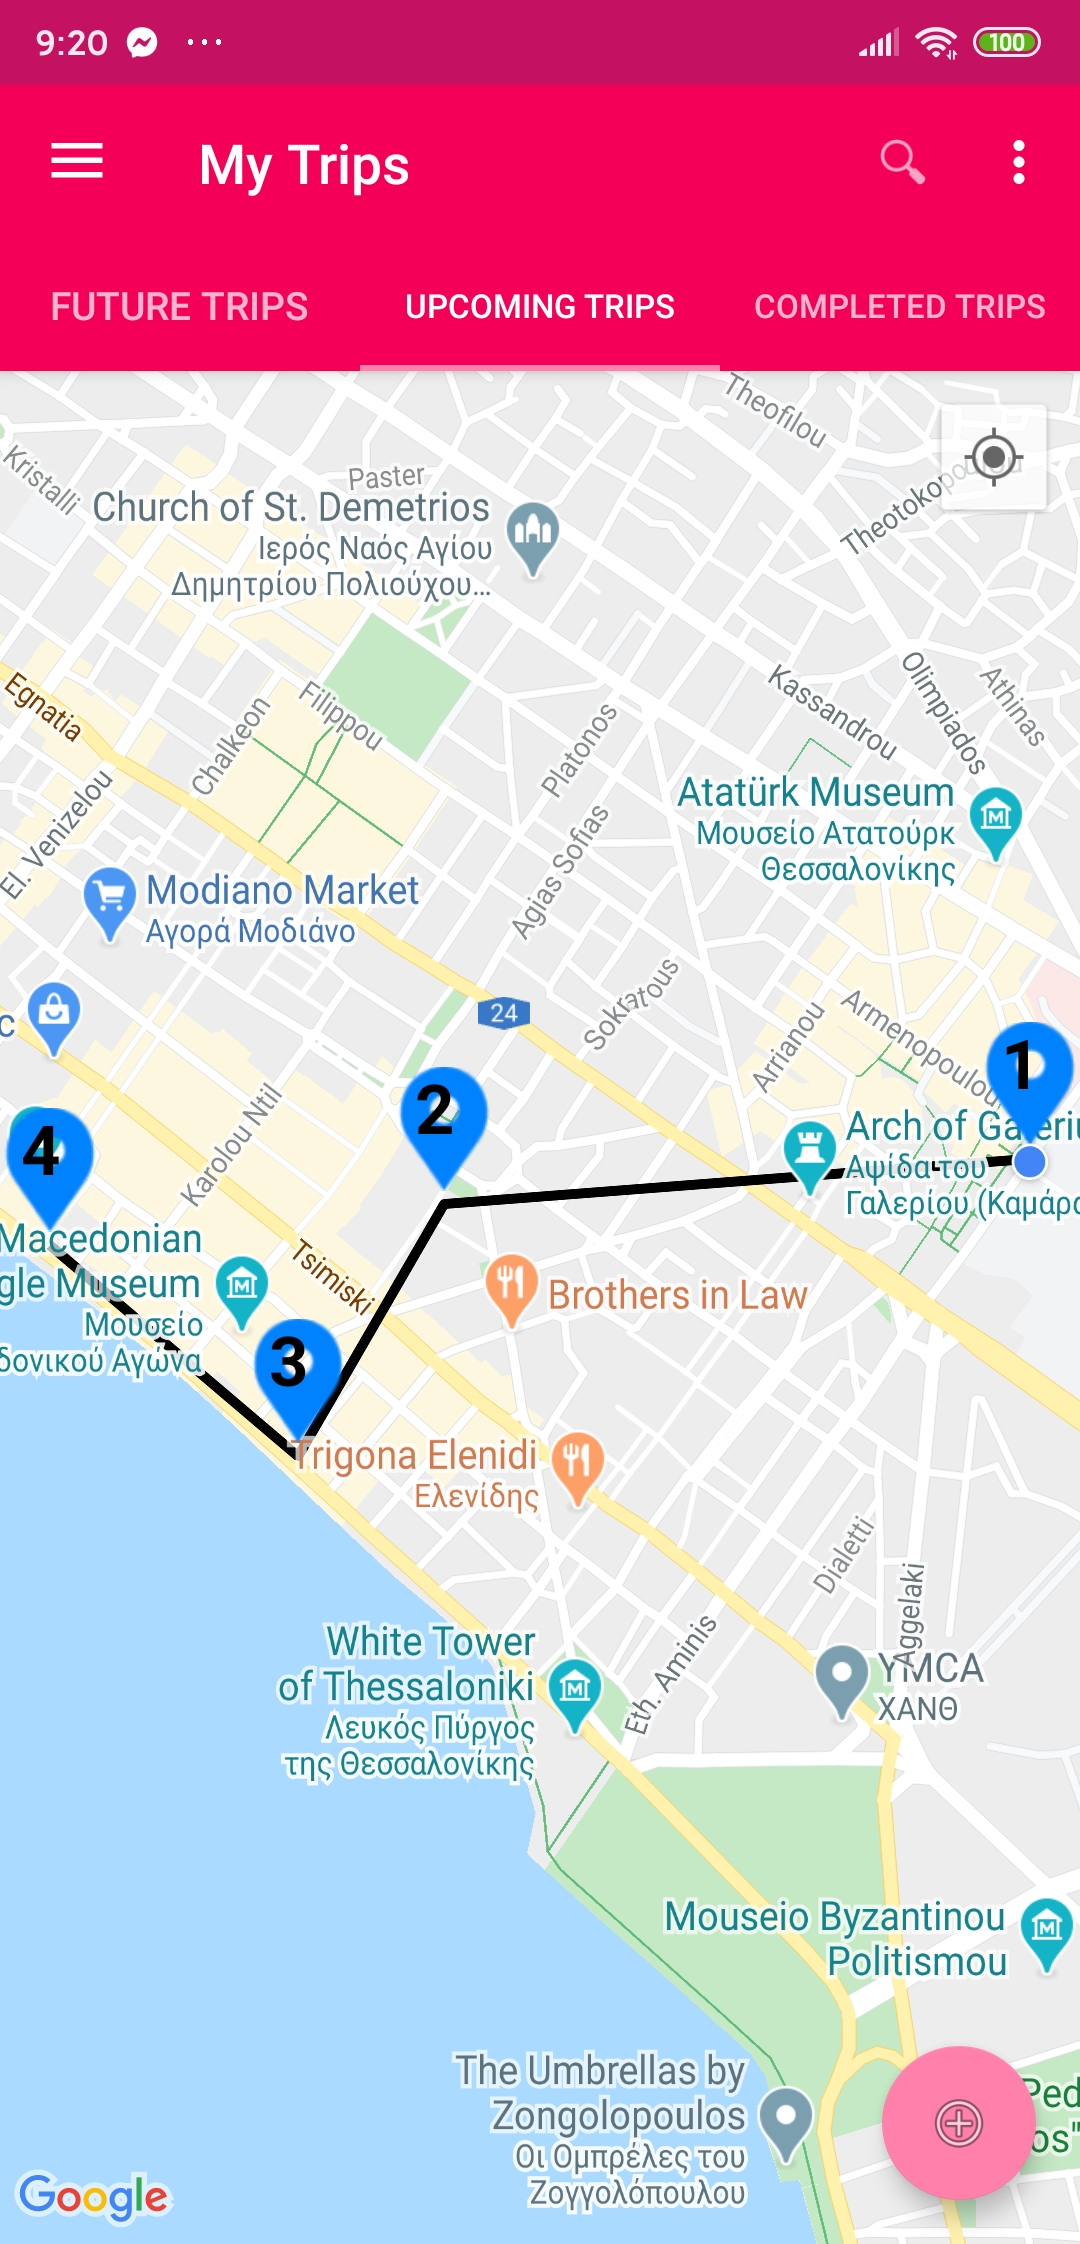
\includegraphics[scale=0.15]{images/shortest_places_dataset.jpg}
    \caption{Προτεινόμενη διαδρομή μετά από έναρξη ταξιδιού}
    \label{fig:shortest_path_dataset}
\end{figure}

Για να βεβαιωθεί ότι κάθε φορά ο αλγόριθμος που περιγράφηκε στην 
ενότητα \ref{sec:start_user_trip} επιστρέφει το ίδιο αποτέλεσμα, 
εκτελέστηκε 100,000 φορές. Επιβεβαιώθηκε πως κάθε φορά επέστρεψε το ίδιο 
αποτέλεσμα.
Ο αλγόριθμος επέστρεψε μία λίστα με τοποθεσίες 
ταξινομημένη με την σειρά την οποία πρέπει να επισκεφθεί ο χρήστης 
την κάθε τοποθεσία. Η λίστα αυτή, φυσικά περιλαμβάνει και την 
αρχική θέση του χρήστη και αναπαρίσταται από το διάγραμμα \ref{fig:shortest_path_dataset_plain}. Επίσης τα σημεία αυτά 
χρησιμοποιούν ως αναφορά τις εγγραφές του πίνακα 
\ref{table:shortest_places_dataset}.

\tikzstyle{clientarrow} = [->,thick,>=triangle 90]

\begin{figure}[h]
\centering
\begin{tikzpicture}[node distance=3cm]
    \node(place1) [clientblock] {Αρχική θέση};
    \node(place2) [clientblock, right of=place1] {C};
    \node(place3) [clientblock, right of=place2] {B};
    \node(place4) [clientblock, right of=place3] {A};
    
    \draw [clientarrow] (place1) -- (place2);
    \draw [clientarrow] (place2) -- (place3);
    \draw [clientarrow] (place3) -- (place4);
\end{tikzpicture}
\caption{\label{fig:shortest_path_dataset_plain} Βέλτιστη διαδρομή μεταξύ των τοποθεσιών}
\end{figure}

Έπειτα, για να επιβεβαιωθεί ότι η διαδρομή που προτάθηκε ήταν όντως 
η βέλτιστη, αναλύθηκαν όλες οι πιθανές διαδρομές με τη συνολική τους απόσταση. Τα αποτελέσματα της ανάλυσης περιγράφονται παρακάτω στον πίνακα \ref{table:shortest_places_dataset_analysis}.

\begin{table}[H]
\centering
    \begin{tabular}{|c|c|c|c|c|}
        \hline
        \textbf{Τοπ. 1} & \textbf{Τοπ. 2} & \textbf{Τοπ. 3} & \textbf{Τοπ. 4} &  \textbf{Συνολική απόσταση} \\
        \hline
        I & A & B & C & 2.3km \\
        \hline
        I & A & C & B & 2.5km \\
        \hline
        I & B & A & C & 2.3km \\
        \hline
        I & B & C & A & 2.3km \\
        \hline
        I & C & A & B & 2.0km \\
        \hline
        \rowcolor{yellow!40} I & C & B & A & 1.7km \\
        \hline
    \end{tabular}
    \caption{Αποτέλεσμα ανάλυσης βέλτιστης διαδρομής για τις δοσμένες γεωγραφικές συντεταγμένες\label{table:shortest_places_dataset_analysis}}
\end{table}

Όπως φαίνεται και στον πίνακα παραπάνω, η διαδρομή που προτάθηκε 
από την εφαρμογή είναι και η βέλτιστη. Επιπλέον, αξίζει να 
σημειωθεί πως για την εξαγωγή της συνολικής απόστασης για κάθε 
πιθανή διαδρομή χρησιμοποιήθηκε το Directions API από τους χάρτες 
της Google. Στο συγκεκριμένο API, επιλέχθηκε η μετάβαση στα 
επιλεγμένα σημεία ως πεζός. Το Directions API λαμβάνει υπόψιν του 
τους δρόμους και τα εμπόδια που θα εντοπιστούν στην διαδρομή, οπότε 
προσαρμόζεται ανάλογα η συνολική απόσταση. Αντίθετα, ο αλγόριθμος 
που αναπτύχθηκε υπολογίζει την απόσταση μεταξύ δύο σημείων σε 
απόλυτη ευθεία. Σε κάποιες πολύ συγκεκριμένες και λίγες 
περιπτώσεις, ο αλγόριθμος θα βγάλει λανθασμένο αποτέλεσμα καθώς θα 
υπάρξουν εμπόδια που θα αναγκάσουν το χρήστη να διανύσει μεγαλύτερη 
απόσταση.

\section{Έλεγχος κατηγοριοποίησης τοποθεσιών}
Στην ενότητα \ref{sec:location_categorization} περιγράφηκε ο τρόπος 
κατά τον οποίο γίνεται η κατηγοριοποίηση των τοποθεσιών. Ωστόσο, 
ήταν αναγκαίο να ελεγχθεί εάν η μέθοδος που χρησιμοποιήθηκε για να 
μπουν οι κατηγορίες στις τοποθεσίες έβγαζε λογικά και σωστά 
αποτελέσματα.

Παίρνοντας τα δεδομένα των τοποθεσιών του πίνακα \ref{table:shortest_places_dataset}, οι κατηγορίες για την κάθε τοποθεσία βρίσκονται παρακάτω

\begin{table}[H]
\centering
    \begin{tabular}{|c|c|c|c|c|}
        \hline
        \textbf{\#} & \textbf{Τοποθεσία} & \textbf{Latitude} & \textbf{Longitude} & \textbf{Κατηγορία} \\
        \hline
        1 & Ernest Hebrard & 40.631749939012 & 22.94103699804 & Coffee, Entertainment\\
        \hline
        2 & Esatto & 40.629498095075 & 22.944526988045 & Coffee, Nightlife \\
        \hline
        3 & Cin Cin & 40.63219 & 22.94658 & Food, Coffee \\
        \hline
    \end{tabular}
    \caption{Επαλήθευση κατηγοριοποίησης τοποθεσιών\label{table:place_categorization_results}}
\end{table}

Για να ελεγχθεί εάν η εφαρμογή πρόσθεσε τις κατάλληλες κατηγορίες στις παραπάνω τοποθεσίες, έγινε μία διασταύρωση με την εφαρμογή του Facebook.
\begin{enumerate}
    \item Η τοποθεσία \#1 του πίνακα \ref{table:place_categorization_results} κατά το Facebook αφορά μία Καφετέρια όπως πολύ σωστά επεσήμανε και η εφαρμογή. Ωστόσο, η εφαρμογή πρόσθεσε στην τοποθεσία αυτή και την κατηγορία ``Διασκέδαση''. Η κατηγορία αυτή ενδεχομένως να μην αφορά άμεσα την τοποθεσία αυτή.
    \item Η τοποθεσία \#2 κατά το Facebook αφορά μία Καφετέρια αλλά κατά το TripAdvisor κατατάσσεται στην κατηγορία της Νυχτερινής Ζωής. Οπότε, όπως φαίνεται οι κατηγορίες που πρόσθεσε η εφαρμογή TripAssistant στην τοποθεσία αυτή είναι σωστές.
    \item Η τοποθεσία \#3 κατά το Facebook αποτελεί ένα Κοκτέιλ Μπαρ, Εστιατόριο και Καφέ. Όπως φαίνεται και σε αυτή την τοποθεσία, οι κατηγορίες που πρόσθεσε η εφαρμογή είναι σωστές και λογικές.
\end{enumerate}
Όπως αναλύθηκε και παραπάνω, η εφαρμογή TripAssistant εφάρμοσε σωστή κατηγοριοποίηση στις τοποθεσίες, με κάποιες μικρές παρεκκλίσεις όπου προστέθηκαν σε μία τοποθεσία κατηγορίες που δεν ήταν σχετικές με την τοποθεσία αυτή.

\chapter{Συμπεράσματα}

\section{Μελλοντική ανάπτυξη}
Είναι γεγονός πως δεν αναπτύχθηκαν όλες οι λειτουργίες που είχαν 
προγραμματιστεί για την εφαρμογή της πτυχιακής εργασίας, καθώς ο 
χρόνος δεν επαρκούσε. Οι λειτουργίες που δεν ολοκληρώθηκαν 
περιγράφονται παρακάτω στα σχέδια για τη μελλοντική ανάπτυξη της 
εφαρμογής. Κάποιες από αυτές τις λειτουργίες είχαν σχεδιαστεί εξ 
αρχής να υλοποιηθούν, ενώ κάποιες άλλες προέκυψαν κατά τη διάρκεια 
της ανάπτυξης.

\subsection{Υποστήριξη περισσότερων πόλεων}
Όπως έχει αναφερθεί και σε προηγούμενες ενότητες, η εφαρμογή την 
παρούσα στιγμή υποστηρίζει μόνο την πόλη της Θεσσαλονίκης. 
Σε περίπτωση που χρησιμοποιηθεί η εφαρμογή από χρήστη που βρίσκεται 
εκτός της Θεσσαλονίκης, τότε θα λάβει τα αντίστοιχα μηνύματα που θα 
ενημερώνουν πως οι εκάστοτε λειτουργίες δεν είναι διαθέσιμες.
Υποστηρίζοντας περισσότερες πόλεις στην εφαρμογή TripAssistant, 
αυτομάτως διευρύνεται και το κοινό στο οποίο απευθύνεται.

Ο τρόπος που υλοποιήθηκε η υποστήριξη των πόλεων στην εφαρμογή, 
καθιστά πολύ εύκολη την επέκταση των υποστηριζόμενων πόλεων. 
Η κύρια αλλαγή είναι να προστεθεί το όνομα της νέας πόλης μαζί με 
τις γεωγραφικές συντεταγμένες της σε ένα συγκεκριμένο enum.
Φυσικά, αυτή η διαδικασία θα μπορούσε να απλουστευθεί περαιτέρω προσθέτοντας νέες πόλεις στην εφαρμογή μέσω ενός πίνακα ελέγχου. Με αυτό τον τρόπο δεν θα χρειάζονταν νέες αλλαγές στον πηγαίο κώδικα της εφαρμογής καθώς και δημιουργία μίας νέας έκδοσης.
% Βελτίωση της περιήγησης μέσα στους χάρτες
\subsection{Βελτίωση της λειτουργίας έναρξης ταξιδιού χρήστη}
Μία πολύ ενδιαφέρουσα λειτουργία που αναπτύχθηκε είναι αυτή που 
περιγράφεται στην ενότητα \ref{sec:start_user_trip}. Ο χρήστης έχει 
τη δυνατότητα να ξεκινήσει ένα ταξίδι που έχει προγραμματίσει και η 
εφαρμογή προτείνει την πιο γρήγορη διαδρομή στον χρήστη.

Μία αλλαγή που μπορεί να γίνει στο μέλλον είναι η βελτίωση της 
περιήγησης στους χάρτες αφότου έχει γίνει έναρξη ενός ταξιδιού. Πιο 
συγκεκριμένα, αυτή τη στιγμή δεν υπάρχει ζωντανή ενημέρωση για την 
εξέλιξη του ταξιδιού και για τον αριθμό των τοποθεσιών που έχει 
επισκεφθεί ήδη ο χρήστης. Αυτό θα μπορούσε να βελτιωθεί δείχνοντας 
ζωντανά την τρέχουσα τοποθεσία του χρήστη στο χάρτη. Επίσης, οι 
τοποθεσίες που έχει ήδη επισκεφθεί ο χρήστης θα ήταν χρήσιμο να 
λαμβάνουν τη σχετική ένδειξη στον χάρτη. Τέλος, η εφαρμογή θα 
μπορούσε να δώσει την ευκαιρία στον χρήστη να διαγράψει τοποθεσίες 
από ένα ταξίδι το οποίο έχει ήδη ξεκινήσει.

% Δημιουργία chat για συνομιλία μεταξύ χρηστών
\subsection{Δημιουργία chat για συνομιλία μεταξύ των χρηστών}
Στον αρχικό σχεδιασμό των λειτουργιών της εφαρμογής, είχε προστεθεί 
και η δημιουργία chat rooms μέσα στην εφαρμογή ώστε οι χρήστες να 
συνομιλούν μεταξύ τους και να ανταλλάσσουν ιδέες και προτάσεις για 
τις τοποθεσίες μίας πόλης. Θα υπάρχει ένα chat room για κάθε πόλη 
που υποστηρίζει η εφαρμογή, ώστε ένας χρήστης να έχει τη δυνατότητα 
να ζητήσει προτάσεις από τοποθεσίες που θα μπορούσε να επισκεφθεί 
με το ταξίδι του στην πόλη που επιθυμεί. 

Φυσικά, η συγκεκριμένη λειτουργία μπορεί να αναπτυχθεί και 
επεκταθεί αρκετά. Μία ιδέα είναι ότι μπορεί να δοθεί η ευκαιρία 
στον χρήστη να ακολουθήσει τα chat rooms που τον ενδιαφέρουν ώστε 
να λαμβάνει ειδοποιήσεις από τα μηνύματα που στέλνονται σε αυτό. 
Επίσης, θα μπορούσε ένας χρήστης να δημιουργήσει μια προσωπική 
συνομιλία με έναν άλλο χρήστη της εφαρμογής.

\subsection{Σύνδεση με το Wikipedia για λήψη πληροφοριών}
Μία λειτουργία που θα ενίσχυε την εμπειρία του χρήστη είναι και η σύνδεση με το API του Wikipedia ώστε να λαμβάνονται πληροφορίες για τις τοποθεσίες που επιθυμεί να επισκεφτεί ο χρήστης. 

Μέχρι στιγμής, ένας χρήστης έχει στη διάθεσή του το όνομα και τις φωτογραφίες της τοποθεσίας. Ωστόσο, αυτές οι πληροφορίες ενδεχομένως να μην είναι αρκετές για να καταλάβει ένας χρήστης εάν τον ενδιαφέρει να επισκεφτεί την εκάστοτε τοποθεσία οπότε ίσως χρειαστεί να αναζητήσει περαιτέρω πληροφορίες για την τοποθεσία από μία τρίτη εφαρμογή. Πέραν τούτου, κατά την διάρκεια της πλοήγησης ενός χρήστη μεταξύ των τοποθεσιών ενός ταξιδιού του θα ήταν χρήσιμο να βλέπει πληροφορίες για τις τοποθεσίες που επισκέπτεται.

Συνδέοντας την εφαρμογή με το API του Wikipedia, θα μπορούσαν να ληφθούν οι σχετικές πληροφορίες για την εκάστοτε τοποθεσία.  
Για παράδειγμα, ένας χρήστης έχει επισκεφθεί ένα ιστορικό κτήριο και κατά τη διάρκεια της επίσκεψής του διαβάζει μέσω της εφαρμογής TripAssistant πληροφορίες για το κτήριο αυτό.

\section{Συμπεράσματα}
Ύστερα από την περάτωση της παρούσας πτυχιακής εργασίας βγήκαν κάποια ενδιαφέροντα συμπεράσματα για τη χρησιμότητα των δεδομένων από τα δημόσια APIs.
Πιο συγκεκριμένα, στα πλαίσια της εφαρμογής της πτυχιακής χρησιμοποιήθηκαν κάποια δεδομένα από δημόσια APIs από τα οποία
μπορέσαμε να εξάγουμε πολλές πληροφορίες οι οποίες είναι χρήσιμες για έναν τουρίστα. 
Με τα δεδομένα αυτά μπορούν να εξαχθούν προτάσεις για μέρη που μπορεί να επισκεφθεί ένας τουρίστας, να ληφθούν πληροφορίες για 
την ιστορία ενός μνημείου όπως και πολλά άλλα.

Φυσικά, τα δεδομένα από τα δημόσια APIs δεν είναι χρήσιμα μόνο για την εξαγωγή τουριστικών πληροφοριών. 
Τα δεδομένα που εξάγονται από τα δημόσια APIs μπορούν να χρησιμεύσουν σε πληθώρα εφαρμογών οι οποίες 
περιορίζονται μόνο από την φαντασία των προγραμματιστών που θα τις αναπτύξουν.
Επιπλέον, ο συνδυασμός των δεδομένων που παρέχονται από διαφορετικά δημόσια APIs μπορούν να συνδυαστούν ώστε να δημιουργήσουν ένα μεγαλύτερο και ισχυρότερο σύνολο από δεδομένα.

Μία ακόμα διαπίστωση που έγινε μετά την περάτωση της πτυχιακής εργασίας είναι η χρησιμότητα εφαρμογής των ευέλικτων μεθοδολογιών στην ανάπτυξη ενός project.
Πιο συγκεκριμένα, η χρήση της μεθοδολογίας Scrum και η οργάνωση των επαναλήψεων (Sprints) βοήθησε στην σωστή οργάνωση του project αλλά και στη συνεχή παράδοση νέων εκδόσεων και λειτουργιών.
Έχοντας κάποιες συγκεκριμένες λειτουργίες προς ανάπτυξη σε κάθε επανάληψη, είναι ορισμένη η δουλειά που χρειάζεται να γίνει και συνήθως αναπτύσσονται οι λειτουργίες στον προβλεπόμενο χρόνο. Αυτό έχει ως αποτέλεσμα τη συνεχή παράδοση νέων εκδόσεων της εφαρμογής, παίρνοντας έτσι συχνά την γνώμη των ιδιοκτητών του project.
Σε αντίθετη περίπτωση όπου δεν χρησιμοποιείται μια ευέλικτη μεθοδολογία, η ομάδα και οι προγραμματιστές συνήθως καθυστερούν την παράδοση των εκδόσεων του λογισμικού έχοντας ως αποτέλεσμα πολλές φορές πολλές φορές την μη ικανοποίηση των ιδιοκτητών του project για το τελικό αποτέλεσμα.

Τέλος, πολύ χρήσιμα στον κύκλο ζωής ενός έργου φάνηκαν και τα συστήματα Continuous Integration/Continuous Delivery.
Χρησιμοποιώντας ένα τέτοιο σύστημα διασφαλίζεται και βελτιώνεται σημαντικά η ποιότητα του λογισμικού που παραδίδεται.

%Προαιρετικά
\begin{Glossary}
%Το γλωσσάρι μπορεί να είναι χρήσιμο αν χρησιμοποιείτε πολλά ακρώνυμα
%και συντομογραφίες.
\begin{description}
\item[API] Application Programming Interface
\item[WSDL] Web Services Description Language
\item[WS] Web Service
\item[RPC] Remote Call Procedure
\item[HTTP] Hypertext Transfer Protocol
\item[FCM] Firebase Cloud Messaging
\item[REST] Representational State Transfer
\item[SQL] Structured Query Language
\item[JSON] JavaScript Object Notation  
\item[URL] Uniform Resource Locator (Μία διεύθυνση ενός πόρου του παγκοσμίου Ιστού)
\end{description}
\end{Glossary}

\printbibliography

\lastpageinfo
\end{document}
